\documentclass[thesis,tocnosub,noragright,centerchapter,12pt]{uiucecethesis09}

% Use draftthesis for notes and date markings on every page.  Useful when you
%   have multiple copies floating around.
% Use offcenter for the extra .5 inch on the left side. Needed with fullpage and fancy.
% Use mixcasechap for compatibility with hyperref package, which does NOT like all caps default
% Use edeposit for the adviser/committee on the title page.
% Use tocnosub to suppress subsection and lower entries in the TOC.
% PhD candidates use "proquest" for the proquest abstract.

\makeatletter

%%%%%%%%%%%%%%%
% MK Added to make bib work
% MK removed on 1/8/19
% \bstctlcite{IEEEexample:BSTcontrol}

% MK added to highlight stuff
\usepackage{color,soul}

% MK added so figures can use the [H] option and be put where I want them.
\usepackage{float}

% MK added so algorithms work
\usepackage{algorithm}

%%%%%%%%%%%%%%%

\setcounter{secnumdepth}{5} % to make subsubsections work
\usepackage{setspace}
\usepackage{epsfig}  % for figures
\usepackage{graphicx}  % another package that works for figures
\usepackage{subfigure}  % for subfigures
\usepackage{amsmath}  % for math spacing
\usepackage{amssymb}  % for math spacing
%\usepackage{url}  % Hyphenation of URLs.
\usepackage{lscape}  % Useful for wide tables or figures.
\usepackage[justification=raggedright]{caption}	% makes captions ragged right - thanks to Bryce Lobdell


\DeclareMathOperator*{\argminA}{arg\,min} % Jan Hlavacek

% Uncomment the appropriate one of the following four lines:
%\msthesis
\phdthesis
%\otherdoctorate[abbrev]{Title of Degree}
%\othermasters[abbrev]{Title of Degree}

\title{Automated Isotope Identification Algorithm Using Artificial Neural Networks}
\author{Mark Kamuda}
\department{Nuclear Plasma and Radiological Engineering}
%\department{\mbox{Nuclear, Plasma, and Radiological Engineering}}
\degreeyear{2019}

% Advisor name is required for
% - doctoral students for the ProQuest abstract
% - master's students who do not have a master's committee
% \advisor{Assistant Professor Clair J. Sullivan}

% Uncomment the \committee command for
% - all doctoral students
% - master's students who have a master's committee
\committee{Kathryn Huff, Adviser\\
        Rizwan Uddin\\
        Tomasz Kozlowski\\
        Clair Sullivan\\
        Mark Hasagawa-Johnson}





\begin{document}

%%%%%%%%%%%%%%%%%%%%%%%%%%%%%%%%%%%%%%%%%%%%%%%%%%%%%%%%%%%%%%%%%%%%%%%%%%%%%%%
% COPYRIGHT
%
%\copyrightpage
%\blankpage

%%%%%%%%%%%%%%%%%%%%%%%%%%%%%%%%%%%%%%%%%%%%%%%
%%%%%%%%%%%%%%%%%%%% TITLE %%%%%%%%%%%%%%%%%%%%
%%%%%%%%%%%%%%%%%%%%%%%%%%%%%%%%%%%%%%%%%%%%%%%
\maketitle
%\raggedright
\parindent 1em%
\frontmatter

%%%%%%%%%%%%%%%%%%%%%%%%%%%%%%%%%%%%%%%%%%%%%%%
%%%%%%%%%%%%%%%%%%% ABSTRACT %%%%%%%%%%%%%%%%%%
%%%%%%%%%%%%%%%%%%%%%%%%%%%%%%%%%%%%%%%%%%%%%%%
\begin{abstract}
There is a need to develop an algorithm that can identify and quantify isotopes in low-resolution gamma-ray spectra. Trained gamma-ray spectroscopists typically rely on intuition when identifying isotopes in spectra. Because they incorporate something similar to the intuition used by trained spectroscopists, pattern recognition algorithms such as neural networks are prime candidates for automated isotope identification. Algorithms based on feature extraction such as peak finding or ROI algorithms work well for well-calibrated high resolution detectors. For low-resolution detectors, it may be more beneficial to use algorithms that incorporate more abstract features of the spectrum. To investigate this, an artificial neural network (ANN) was trained to predict the presence and relative activities of isotopes from gamma-ray spectra. The ANN is trained with simulated gamma-ray spectra, allowing easy expansion of the library of target isotopes. This proposal outlines extensions to this work including investigating new datasets and ANN structures.



\end{abstract}


%%%%%%%%%%%%%%%%%%%%%%%%%%%%%%%%%%%%%%%%%%%%%%%
%%%%%%%%%%%%%%%%%% DEDICATION %%%%%%%%%%%%%%%%%
%%%%%%%%%%%%%%%%%%%%%%%%%%%%%%%%%%%%%%%%%%%%%%%
%\begin{dedication}
%To my parents, for their love and support.
%\end{dedication}

%%%%%%%%%%%%%%%%%%%%%%%%%%%%%%%%%%%%%%%%%%%%%%%
%%%%%%%%%%%%%%% ACKNOWLEDGMENTS %%%%%%%%%%%%%%%
%%%%%%%%%%%%%%%%%%%%%%%%%%%%%%%%%%%%%%%%%%%%%%%
\begin{acknowledgments}
Acknowledgments text. 
\end{acknowledgments}

%%%%%%%%%%%%%%%%%%%%%%%%%%%%%%%%%%%%%%%%%%%%%%%
%%%%%%%%%%%%%% TABLE OF CONTENTS %%%%%%%%%%%%%%
%%%%%%%%%%%%%%%%%%%%%%%%%%%%%%%%%%%%%%%%%%%%%%%
\tableofcontents

%%%%%%%%%%%%%%%%%%%%%%%%%%%%%%%%%%%%%%%%%%%%%%%
%%%%%%%%%%%%%%% LIST OF TABLES %%%%%%%%%%%%%%%%
%%%%%%%%%%%%%%%%%%%%%%%%%%%%%%%%%%%%%%%%%%%%%%%
% The List of Tables is not strictly necessary. Omitting the List of Tables will
% simplify the thesis check and reduce the number of corrections.
\listoftables

%%%%%%%%%%%%%%%%%%%%%%%%%%%%%%%%%%%%%%%%%%%%%%%
%%%%%%%%%%%%%%% LIST OF FIGURES %%%%%%%%%%%%%%%
%%%%%%%%%%%%%%%%%%%%%%%%%%%%%%%%%%%%%%%%%%%%%%%
% The List of Figures is not strictly necessary. Omitting the List of Figures will
% simplify the thesis check and reduce the number of corrections.
\listoffigures

%%%%%%%%%%%%%%%%%%%%%%%%%%%%%%%%%%%%%%%%%%%%%%%
%%%%%%%%%%% LIST OF ABBREVIATIONS %%%%%%%%%%%%%
%%%%%%%%%%%%%%%%%%%%%%%%%%%%%%%%%%%%%%%%%%%%%%%
% The List of Abbreviations is not strictly necessary.
%\chapter{LIST OF ABBREVIATIONS}

%\begin{symbollist*}
%\item[DNN] Dense Neural Network
%\item[CNN] Convolution Neural Network
%\end{symbollist*}

%%%%%%%%%%%%%%%%%%%%%%%%%%%%%%%%%%%%%%%%%%%%%%%
%%%%%%%%%%%%%% LIST OF SYMBOLS %%%%%%%%%%%%%%%%
%%%%%%%%%%%%%%%%%%%%%%%%%%%%%%%%%%%%%%%%%%%%%%%
%\begin{symbollist}[0.7in]
%\item[$\tau$] Time taken to drink one cup of coffee.
%\end{symbollist}

\mainmatter

%%%%%%%%%%%%%%%%%%%%%%%%%%%%%%%%%%%%%%%%%%%%%%%
%%%%%%%%%%%%%%%%%%%%%%%%%%%%%%%%%%%%%%%%%%%%%%%
%%%%%%%%%%%%%%%%%%%%%%%%%%%%%%%%%%%%%%%%%%%%%%%
%%%%%%%%%%%%%%%% THESIS BODY %%%%%%%%%%%%%%%%%%
%%%%%%%%%%%%%%%%%%%%%%%%%%%%%%%%%%%%%%%%%%%%%%%
%%%%%%%%%%%%%%%%%%%%%%%%%%%%%%%%%%%%%%%%%%%%%%%
%%%%%%%%%%%%%%%%%%%%%%%%%%%%%%%%%%%%%%%%%%%%%%%

\chapter{Introduction}

\section{Introduction and Motivation}

Gamma-ray spectroscopy plays an important role in homeland security and nonproliferation technologies. By analyzing the gamma-ray spectrum of some material, naturally occurring radioactive material (NORM) can be distinguished from threat isotopes. Threat isotopes include undeclared industrial, medical, and special nuclear material (SNM) sources that can be used in a dirty bomb or nuclear explosive device. Detecting these materials is the first step to intercepting them and preventing nuclear material proliferation.

% Gamma-ray spectroscopy can also be used to measure uranium enrichment, an important measurement for nonproliferation and nuclear treaty verification. 

Common detection materials for commercial radioisotope identification devices (RIID) are the low-resolution sodium iodide (NaI(Tl)) \cite{Hofstadter1948}, medium-resolution cadmium zinc telluride (CZT), and high-resolution high purity germanium (HPGe). All of these materials have sufficient resolution to perform gamma-ray spectroscopy. While medium- and high-resolution materials offer better performance, they suffer from several drawbacks. These materials cost more and are difficult to manufacture in large volumes. Larger detector volumes have an increased absolute efficiency which reduces measurement times. In addition to these drawbacks, HPGe detectors require cryogenic cooling. This greatly increases the weight and cost of portable HPGe detectors. Despite the reduced resolution, NaI(Tl) is standard in the RIID industry due to its low cost, ability to be manufactured in large volumes, high intrinsic efficiency.

Reported commercial RIID performance is generally poor \cite{pibida2004,blackadar2003,blackadar2004}. One study found that seven commercial RIIDs had an average of less than 50\% correct identifications for SNM, industrial, and medical sources \cite{blackadar2003}. Another study found that a 2 mm stainless steel plate (a moderate amount of shielding) was enough to eliminate correct identifications in four commercially available RIIDs \cite{pibida2004}. Because of the importance of an alarm - and because of inadequate RIID performance - the U.S. Department of Energy (DOE) employs a team of on-call spectroscopists to resolve RIID alarms \cite{burr2009}. Because of their importance, RIID detection systems are in need of improvement.

% large CZT research \cite{Gostilo2004,Chen2018}

RIID improvements fall into two categories: improvements in the quality of the spectrum and improvements in the identification algorithms \cite{swoboda2004}. Spectral quality is largely determined by the energy resolution of the radiation detection material. Improvements in energy resolution often increase manufacturing cost and reduce feasible detector size. Active research into advanced detection materials has not yet produced a material economically competitive with NaI(Tl). Because of this, RIID improvements should focus on the identification algorithms using this industry standard material \cite{blackadar2003}.

This dissertation aims to investigate a novel identification algorithm - machine learning using simulated training data - as a possible avenue of improving the performance of RIIDs using the Ortec 905-3 2- x 2-in. NaI(Tl) cylindrical scintillation detector. Despite widespread use, NaI(Tl) detectors have several issues that complicate automated identification.

The first issue is the low resolution of NaI(Tl). The poor resolution makes some photopeaks unresolvable from each other, complicating identification.

% http://www2.pv.infn.it/~debari/doc/Flyckt_Marmonier.pdf pg.4-36
The second issue is calibration drift due to changes in environmental temperature and voltage drifts in the photomultiplier tube due to changes in count rate \cite{knoll,gilmore}. This drift affects the locations and shapes of features in a gamma-ray spectrum. To solve this, the detector must recalibrate to a reference source (possibly built-in) or a naturally occurring background source. These methods fall short for different reasons. Built-in sources need to be periodically replaced and add an unwanted signal to a spectrum. Recalibration sources can be included separately, requiring the user find this source and periodically recalibrate - complicating practical use. Calibrating from a background reference (typically the 1.460 MeV gamma-ray peak from $^{40}$K or the 2.614 MeV gamma-ray peak from the thorium decay series) requires a significant measurement time for a useful signal-to-noise ratio. Short measurement times common in homeland security measurements make this option infeasible.

The third issue is a non-linear energy response which manifests as a small second order term in the detector's calibration. While not specific to NaI(Tl) detectors, the fourth issue affecting identification algorithms is background radiation from naturally occurring radioactive material (NORM). NORM radiation can change both in intensity and composition based on location and weather. This background signal can obscure features in gamma-ray spectra.

Despite the drawbacks outlined above, our previous published work has demonstrated that ANNs are capable of identifying multiple isotopes in unknown backgrounds with a wide range of calibration settings \cite{kamudaThesis2017, kamuda2017, kamuda2018}. Furthermore, the work presented in this dissertation demonstrates that ANNs are capable of performing both classification and quantification tasks using low-resolution gamma-ray spectra.


% \section{Radioisotope Identification Device Applications}

% Statistical methods applied to gamma-ray spectroscopy algorithms in nuclear security missions \cite{Min2014}.

% \subsection{Homeland Security}

% Handheld RIIDs are used by boarder protection and law enforcement for porthole and area monitoring \cite{Hodge2007}. An example of area monitoring could be monitoring a high traffic area during a high-profile event. An example of porthole monitoring is monitoring cargo vehicles. RIIDs are typically employed in second screening activities, after a primary count rate alarm is triggered. In order to minimize traffic and ensure cargo containers leave in an economically reasonable time, screening activities are kept on the order of minutes. Another example of porthole monitoring is temporary checkpoints where traffic is slowed but not stopped. Often, the important task for devices employed in vehicle screening is determining if a primary alarm came from NORM, a legitimate industrial source, or SNM.


% \cite{fagan2012}

% GRADER PROGRAM https://www.dhs.gov/guidance-grader-program


% RIIDs also can be used to identify orphaned sources.
% https://www-sciencedirect-com.proxy2.library.illinois.edu/science/article/pii/S0969804302002221

% Pozzi great references https://www-sciencedirect-com.proxy2.library.illinois.edu/science/article/pii/S0168900217300074


% DATASET https://www-sciencedirect-com.proxy2.library.illinois.edu/science/article/pii/S0168900214012741

% \subsection{Nuclear Treaty Verification}

% Talk about Zero knowledge measurements 


\section{Neural Network History}


Scientists first theorized artificial neural networks in the 1940s as a model of how complex biological systems like neuron bundles learn and remember \cite{Pitts1943, Hebb1949}. These theories hypothesized that learning takes place by reinforcing neural connections corresponding to some beneficial behavior. The first implementation of an ANN came in 1958 in the form of a machine named The Mark I Perceptron \cite{Rosenblatt1958, Rosenblatt1962}. The Mark I Perceptron was a physical neural network whose weights were changed with motor-controlled potentiometers. The Mark I Perceptron implemented a two-class image recognition problem using a 400-pixel camera. In this context, a class represents an item in a set of mutually exclusive items (e.g. dog/cat or on/off). The device also included an algorithm (the perceptron learning algorithm) to learn optimum weights for a given task. Unfortunately, the single-layer perceptron failed in cases without linearly separable classes in the data because it was based on linear combinations of fixed basis functions \cite{Bishop2006, Minsky1969}. This realization and other perceived flaws led to a temporary decline in neural network research.

% While a single layer perceptron network could only solve linearly separable problems, in 1969 it was also found that a network with multiple layers could solve problems that are non-linearly separable \cite{Minsky1969}. 

% The perceptron algorithm was limited to a single layer network due to its activation function being a non-differentiable step function.

% Another single layer neural network design was ADALINE, created in 1960 \cite{Widrow1960}. While the ADALINE algorithm shares a similar architecture with the perceptron, its learning rule differs. It was soon shown that multiple ADALINE neurons could be stacked on top of each other, creating a MADALINE network \cite{Ridgway1962}. Due to its multilayer structure, MADALINE is able to learn non-linearly separable functions. A MADALINE network was used as an adaptive filter that removes echo from phone lines \cite{Widrow1988}.

Further advances were made when Rumelhart et al. formalized error backpropagation and it's application to training ANNs \cite{Rumelhart1986}. Error backpropogation was found to be a simple and powerful method to update an ANN to learn arbitrary functions. Error backpropogation combined with gradient descent allowed for efficient ANN training. Algorithms based on the backpropogation of error are now the most common method to train ANNs. % Additionally, it was shown that error backpropogation applied with a differentiable non-linear activation function was an extremely powerful method to train ANNs \cite{Murtagh1991}.

Currently, ANNs can solve many, diverse problems. ANNs have shown promise in everyday problems such as handwritten zip code recognition \cite{LeCun1989}, image recognition \cite{Krizhevsky2012}, and fingerprint identification \cite{Jeyanthia2015}; as well as more complicated problems such as lung cancer classification based on MRI images \cite{Selvakumari2016}, estimating surface soil moisture from high-resolution aerial images of cropland \cite{Hassan-Esfahani2015}, and stock market forecasting \cite{Rababaah2015}. 


\section{Gamma-Ray Spectroscopy for Isotope Identification and Quantification}

Rawool-Sullivan et al. identified a common workflow performed by a group of trained gamma-ray spectroscopists \cite{RawoolSullivan2010}. This workflow includes discriminating source photopeaks from the background signal, adjusting the calibration using background photopeaks, and checking for shielding effects in the low-energy photopeaks. Once the spectroscopist identifies photopeaks, they use prior knowledge or consult a database of isotope decay energies to identify isotopes in the spectrum. The researchers noted that spectroscopists often employ a mixture of factual knowledge and intuition developed from analyzing tens or hundreds of gamma-ray spectra in their analysis. The researchers also noted the difficulty in incorporating this subjective analysis into an automated algorithm.
% This is one of the main arguments for using ANNs in automated isotope ID

Many automated radioisotope identification methods are available, but few perform well given a low-resolution gamma-ray spectrum of a mixture of radioisotopes. Automated RIID methods used in such scenarios include library comparison algorithms, region of interest (ROI) algorithms, principle component analysis (PCA), and template matching. While these algorithms may work well in laboratory settings, they often offer unacceptable performance in more realistic conditions.

Library comparison algorithms attempt to match photopeak energies found in a gamma-ray spectrum with those found in a library of known isotope decay energies. Drifts and uncertainties in detector calibration can lead to misidentifying photopeaks, leading to incorrect isotope identifications \cite{burr2009}. To automate this method, a separate algorithm is required to extract photopeak centroids in the presence of calibration drift and an unknown background signal. While research on methods for photopeak extraction are ongoing \cite{mariscotti1967,DELOTTO1977,GARDNER2011}, they face difficulties when a large number of photopeaks overlap in a spectrum \cite{xiong2015}, such as when a low-resolution detector measures a mixture of radio-isotopes.

ROI algorithms define regions in a spectrum where they expect target radioisotope photopeaks. These algorithms then compare counts in these regions to a measured or expected background. Significant elevation in counts in a target isotopes ROIs indicates the presence of that isotope. Similar to library comparison algorithms, ROI algorithms operate poorly when photopeaks of different radioisotopes overlap \cite{burr2009}. Because of this, large isotope libraries perform poorly using this method. Similarly to the library comparison algorithm, calibration drift may shift photopeaks into neighboring ROIs, leading to incorrect identification. Despite drawbacks, an ROI method has been used to differentiate normally occurring radioactive material (NORM) from special nuclear material (SNM) using plastic scintillators \cite{Ely2006}.

PCA can also be applied to radioisotope identification. PCA aims to reduce a dataset's dimensionality into uncorrelated variables \cite{Jolliffe2002}. Using a subset of these principle components, the data may be represented in a reduced space of orthogonal bases that contains most of the information present in the original data. Isotopes in the the transformed data can then be clustered using methods like K-means, Mahalanobis distance, or k-nearest neighbors \cite{Kanungo2002, Kumari2012}. PCA has been applied to isotope identification using plastic scintillators \cite{Boardman2012} and anomaly detection using both plastic scintillators and NaI(Tl) detectors \cite{runkle2006b}. Despite PCA's progress in some isotope identification problems, application using PCA to separating isotope mixtures in gamma-ray spectra could not be found.

Template matching algorithms find an example in a database of gamma-ray spectra that most closely matches a measured spectrum \cite{burr2009}. The spectral database can contain multiple detector calibration settings, shielding materials, and source-to-detector distances. Quality of fit can be measured using a hypothesis test such as chi-squared test or correlation coefficient. While a sufficiently large spectral database can theoretically be used to identify almost any measured spectrum, the drawback of this method is the time necessary to compare a measured spectrum to the library and the computer memory necessary to store said library. Despite the drawbacks, researchers have made progress applying a multiple linear regression procedure to identify mixtures of isotopes using template matching \cite{mattingly2010}.

The algorithms described previously largely incorporate book knowledge. The present work is motivated by the notion that incorporating the intuition identified by Rawool-Sullivan et al. can improve these algorithms. By carefully creating a training set of spectra and intelligently applying deep learning, a machine learning approach to automated gamma-ray spectroscopy may be succeed in marrying book knowledge and a trained spectroscopists intuition.


\section{Automated Isotope Identification Using ANNs}

A number of published papers apply ANNs to automated isotope identification. ANNs have been applied to peak fitting \cite{Abdel-Aal2002}, isotope identification \cite{Abdel-Aal1996, Medhat2012}, and activity estimation \cite{Abdel-Aal1996, Vigneron1996}. Many of these publications rely on ROI methods \cite{Pilato1999}, feature extraction \cite{Chen2009}, high-resolution gamma-ray spectra \cite{Yoshida2002}, and small libraries of isotopes. In addition, many assume perfect knowledge of detector calibration. ANN training methods created for high-resolution gamma-ray spectra may not perform well when trained using low-resolution spectra. Because of the large discrepancy in resolution, spectral features exploited by a ANN trained on high-resolution spectra would be different than an ANN trained on low-resolution spectra. In addition, ANN training that relies on ROI methods may not perform well when ROIs overlap significantly (as previously explained). Feature extraction and ROI methods may also falter when the background radiation field is unknown or the detector calibration is unreliable.  

Instead of training an ANN using predetermined ROIs or feature extraction, the present work hypothesizes that it is better to train the ANN with an entire gamma-ray spectrum. Due to perceived training issues and computational requirements associated with using the entire spectrum \cite{Pilato1999,Yoshida2002}, previous work in the gamma-ray spectroscopy community have avoided this approach. However, we have shown that training an ANN using the full spectrum can viably identify and quantify isotopes in gamma-ray spectra \cite{kamuda2017,kamudaThesis2017,kamuda2018}. Evidence in the present work also demonstrates that this method can overcome common gamma-ray spectroscopy issues like calibration shifts and identifying isotopes in spectra without clear spectral features.

% This work suggests performing feature extraction and radioisotope identification simultaneously using an ANN. Skipping automated peak-fitting routines releases the algorithm from the burden of determining proper fitting method for a variety of common challenges. For example, changes based on a given photopeaks location in another photopeak's Compton continuum will change the baseline. The second challenge is in deconvolving multiplets. Peak multiplets occur when photopeaks of a given isotope or mixture of isotopes overlap. Instead of making deterministic rules for each of these cases, a machine learning algorithm can be taught to recognize and handle them automatically.

% One identification method involves Once photopeaks are found, another algorithm is needed to measure the locations of peak centroids and additional information (peak area, area uncertainty) to identify what isotopes are present in a spectrum. This process adds computation time and again suffers from the need to be modified to handle changes in a spectrum as described above. Also, the algorithm that performs identification based on peak information must be tailored to the peak-fitting routine. This requires unique algorithms to be created for different detector materials and sizes, as they change the shape of the spectrum. Using an ANN with an appropriate training set, these problems can be avoided.

Using machine learning for isotope identification and quantification offers many advantages over methods previously explained. The problem of determining the feature extraction technique and optimal algorithm is avoided by training an algorithm to identify the important features of a gamma-ray spectrum and simultaneously perform identification or quantification. Using a machine learning approach also has an advantage in the flexibility of its training set and learning objective. Because this method uses simulated gamma-ray spectra to train the model, it does not restrict the number of isotopes allowed in the library. This allows us to cheaply generate the ANN training set using mixtures of exotic, dangerous, or short-lived isotopes that are not easily accessible. Because the training set and learning objective of a machine learning algorithm are flexible, we can train similar deep learning models to perform diverse tasks like source interdiction or uranium enrichment measurements.

% The isotope library and spectral conditions common for source interdiction with border patrol users are very different from those needed to perform enriched uranium measurements. %Because spectra can be generated with different calibrations, this method can be insensitive to a range of calibration shifts due to temperature change or operator error. This insensitivity would allow isotope identification and quantification to be performed without prior knowledge of the detectors calibration.
% ANNs using feature extraction on 3x3 NaI detector \cite{HE2018}.

\section{Chapter Conclusion}

This work addresses the how to generate a synthetic dataset of gamma-ray spectra for relevant problems in isotope identification and quantification. This work also emphasizes how various ANN architectures perform on these datasets. % Due to their operation, we expect different architectures to perform better on different datasets. % Gamma-ray spectroscopists often use intuition when identifying isotopes in spectra. ANNs mimic this abstract analysis, synthesizing features of a gamma-ray spectrum in non-intuitive ways. Exploiting this intuition may overcome common hurdles encountered by other isotope identification algorithms.

Experiments in this work fall into two categories: advanced simulated datasets and advanced machine learning architectures. The first advanced dataset is based on the the American National Standards Institute performance criteria for hand-held instruments for the detection and identification of radionuclides, ANSI N42-34-2006 \cite{ANSI}. This dataset will incorporate the effects of shielding, calibration drift, and unknown background. The second dataset will be based on a zero knowledge measurement for automated uranium enrichment calculations. We will assess the performance of models trained on both datasets using real and simulated gamma-ray spectra. The machine learning architectures explored will include a dense neural network (DNN), dense autoencoder (DAE), convolutional neural network (CNN), and convolutional autoencoder (CAE).


\chapter{Theory}

\section{Gamma-ray Spectroscopy}

In this section, the physics responsible for the features in gamma-ray spectra are described. Also described are factors that complicate gamma-ray spectroscopy, including changing background radiation fields and temperature effects on detector calibration.

% https://sites.fas.harvard.edu/~phys191r/Bench_Notes/B1/NAI_catalog.pdf page 20 has efficiency uncertainty information

\subsection{Energy Deposition Mechanisms}

When a photon interacts with some radiation detection medium, it deposits some or all of it's energy into the material. There are three main methods of interaction: the photoelectric effect, Compton scattering, and pair production. These effects are energy dependent, as seen in Figure \ref{fig:energy_dependence_interactions}.

If the total of the photon's energy is deposited in the detector, a count is recorded in the spectrum's photopeak. If the photon deposits only a part of it's energy and escapes the detector, a count will be recorded somewhere below the full-energy photopeak.  The following sections describe intrinsic mechanisms that remove counts from the full-energy peak.% Absolute efficiency is also affected by shielding material and source-to-detector distance.

\subsubsection{Photoelectric effect}

The photoelectric effect occurs when a photon is absorbed by an atom in some material. This absorption produces a photoelectron, which has the energy of the photon minus the binding energy of the electron. The photoelectron is typically absorbed by the material, resulting in full-energy deposition. This process also creates a vacancy in the atom of the material. This vacancy is filled by another electron in the material, releasing a characteristic x-ray or Auger electron. Because of their low energies, Auger electrons are typically quickly reabsorbed. The characteristic x-ray can either be reabsorbed by the material or escape.

\begin{figure}[H]
\centering
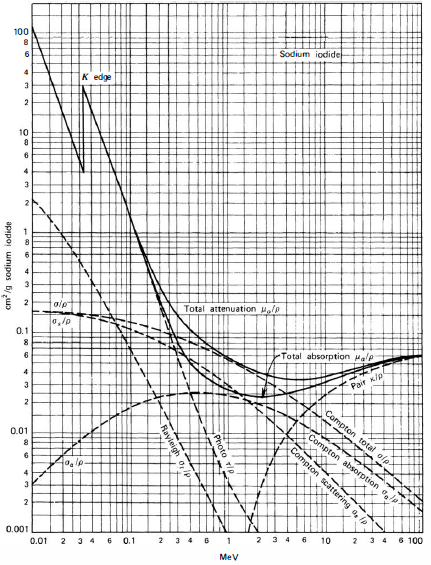
\includegraphics[width=0.75\linewidth]{images/energy_dependence_interactions}
\caption{Energy dependence for gamma-ray interactions in NaI(Tl) \cite{knoll}.}
\label{fig:energy_dependence_interactions}
\end{figure}

\subsubsection{Compton scattering}

Compton scattering and absorption is the interaction of a gamma-ray photon with an electron in some absorbing material. This interaction is illustrated in Figure \ref{fig:compton_scatter}. 


% This is the main energy deposition mechanism in the range of energies useful for gamma-ray spectroscopy.

\begin{figure}[H]
\centering
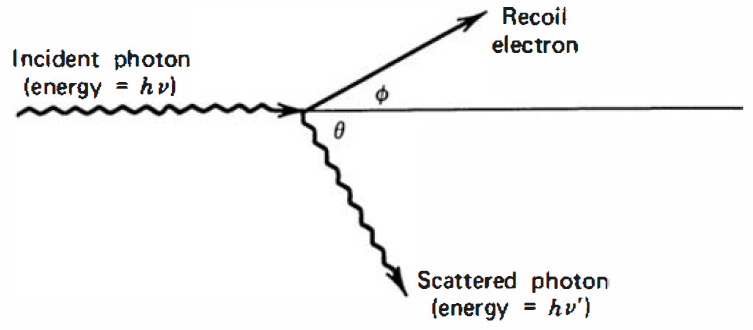
\includegraphics[width=0.7\linewidth]{images/compton_scatter}
\caption{Diagram of a Compton scattering event \cite{knoll}.}
\label{fig:compton_scatter}
\end{figure}

The energy of a photon scattered off a free electron

\begin{equation} \label{eq:compton_scatter}
E' = \frac{E}{1 + \frac{E}{m_{0} c^2} (1-cos\theta)}
\end{equation}

depends on the scattering angle, $\theta$, the incident photon's energy, E, and the rest mass of the electron, m$_{0}$c$^{2}$. A photon scattering at an angle of 180$^{o}$ deposits it's maximum amount of energy into a medium. Photons that escape after this energy deposition create the Compton edge observed at 180$^{o}$, as seen in Figure \ref{fig:ideal_compton}. Photons that escape the detector after single or multiple Compton scatter events at angles less than 180$^{o}$ create the continuum of energies known as the Compton continuum. Accounting for the binding energy of electrons in a medium produces a Compton continuum closer to the dotted line in Figure \ref{fig:ideal_compton}.

\begin{figure}[H]
\centering
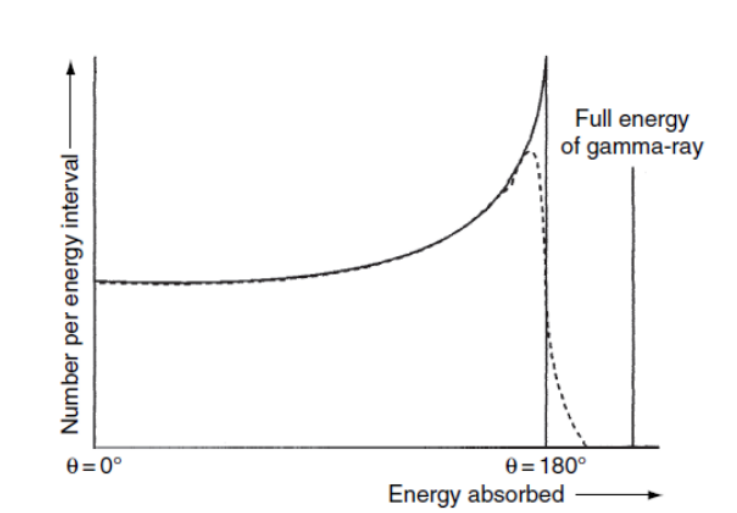
\includegraphics[width=0.75\linewidth]{images/ideal_compton}
\caption{Diagram of energy absorbed in an idealized Compton scattering event \cite{gilmore}.}
\label{fig:ideal_compton}
\end{figure}



\subsubsection{Pair Production}

When a photon with energy above 1022 keV interacts with the coulomb field of a nucleus, there is a probability that the photon will disappear and be replaced by an electron-positron pair. The positron will then annihilate with an electron in the medium, creating two 511 keV photons. This process is illustrated in Figure \ref{fig:pair_production}. Depending if one or both of these annihilation photons escape the detector, they produce single or double escape peaks in a gamma-ray spectrum. As seen in Figure \ref{fig:pair_production_spectra}, single escape peaks occur at 511 keV below the full-energy peak and double escape peaks occur at 1022 keV below this peak. These 511 keV photons may also be measured by the detector, producing an annihilation radiation signal in the spectrum.

\begin{figure}[H]
\centering
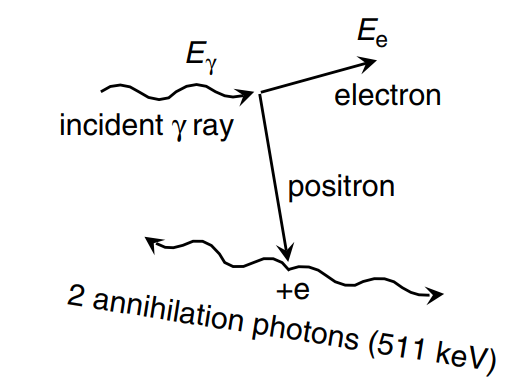
\includegraphics[width=0.6\linewidth]{images/pair_production}
\caption{Diagram of pair production \cite{gilmore}.}
\label{fig:pair_production}
\end{figure}

\begin{figure}[H]
\centering
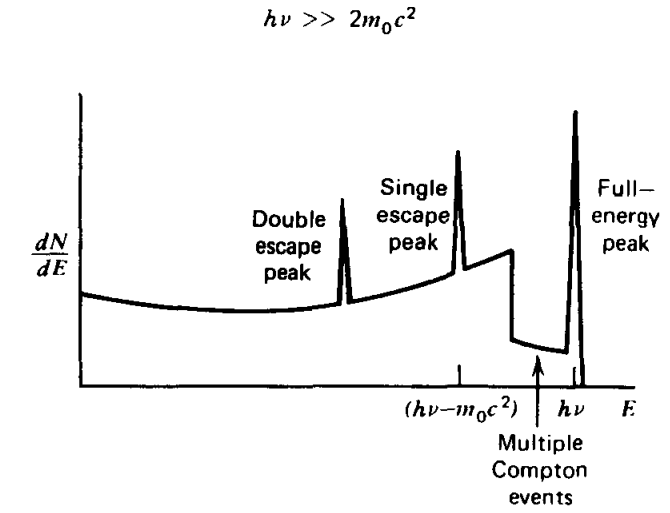
\includegraphics[width=0.6\linewidth]{images/pair_production_spectra}
\caption{Theoretical spectrum from pair production \cite{knoll}.}
\label{fig:pair_production_spectra}
\end{figure}


\subsection{Energy Resolution}

The energy resolution of a radiation detector describes how broad a photopeak is in a spectrum. The resolution is based on the full width of the Gaussian at half of it's maximum value (FWHM). The FWHM is measured either in units of energy or as a percent of the peaks energy. This broadening is mostly due to statistical fluctuations in the number of information carriers produced in the detection system. Other factors that increase the resolution in scintillation detectors include nonproportionality of light yield per energy absorbed, the variance in photoelectron collection in the photocathode, and the variance in electrons produced in the photomultiplier tube \cite{knoll}. Because semiconductor detectors more directly measure charge carriers, they do not suffer the resolution losses associated with transforming information carriers. The variance in information carriers produced for a given energy does not follow a Poisson process in semiconductor detectors. This effect is known as the Fano factor and it significantly decreases the resolution of semiconductor detectors below the theoretical Poisson limit. Because the resolution changes as function of energy, the resolution of a 662 keV photon from $^{137}$Cs is used as a standard for comparison. The energy resolution of three scintillator (NaI(Tl), LaBr, CeBr) and two semiconductor (CZT, HPGe) radiation detectors compared seen in Table \ref{table:detector_resolutions}. Figure \ref{fig:Ba133_spectrum_different_detector_materials_Market_Survey_Report} compares a $^{133}$Ba spectrum from scintillation and semiconductor detectors. 

% pg 345 knoll

\begin{table}[H]
\centering
\begin{tabular}{|c|c|}
\hline
Detector Type & \begin{tabular}[c]{@{}c@{}}Full Width at Half Maximum\\ (662 keV)\end{tabular} \\ \hline
NaI(Tl) & 6 - 8 \% \\ \hline
LaBr & 2 - 4 \% \\ \hline
CeBr & 4 - 5 \% \\ \hline
CZT & 1 - 2 \% \\ \hline
HPGe & \textless 0.2 \% \\ \hline
\end{tabular}
\caption{Typical energy resolutions of different
gamma-ray detector types (reproduced from \cite{RIIDMarketSurveyReport}).}
\label{table:detector_resolutions}
\end{table}


\begin{figure}[H]
\centering
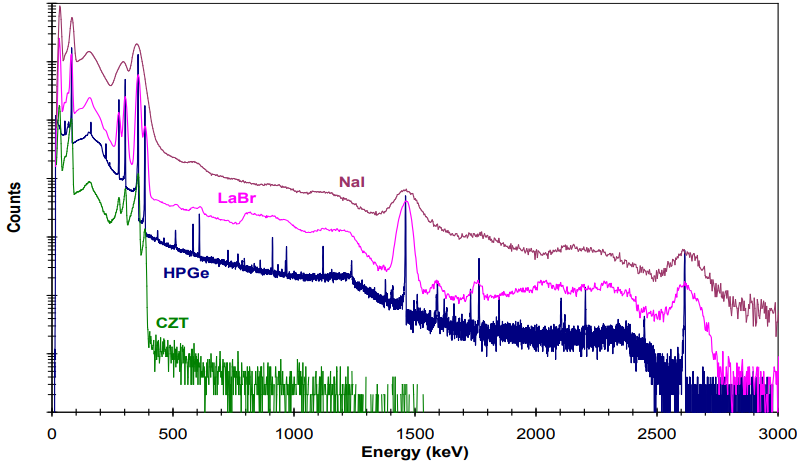
\includegraphics[width=0.8\linewidth]{images/Ba133_spectrum_different_detector_materials_Market_Survey_Report}
\caption{Ba133 spectrum measured using different detector materials \cite{RIIDMarketSurveyReport}.}
\label{fig:Ba133_spectrum_different_detector_materials_Market_Survey_Report}
\end{figure}


\subsection{Background Radiation}

% In contrast, it is extremely difficult to measure a trustworthy background spectrum in the field. Moving or reorienting the detector to obtain a source7free background measurement will frequently produce a measurement that will likely differ significantly, and sometimes even exceeding, the true background at the source position. It is not at all unusual for environmental background to vary significantly over distances of a few meters. As a result, we typically confine our analyses to the foreground spectrum, as generally reflected in this paper. https://e-reports-ext.llnl.gov/pdf/770028.pdf


A significant challenge to automated gamma-ray spectroscopy is the stochastic nature of the background radiation field. Background radiation comes from cosmic radiation and radioisotopes naturally distributed in soil and building materials. Isotopes in the soil come from the uranium decay series, thorium  decay series, and $^{40}$K. The gamma-ray spectra from each of these sources are shown in Figure \ref{fig:background_components}. 

\begin{figure}[H]
\centering
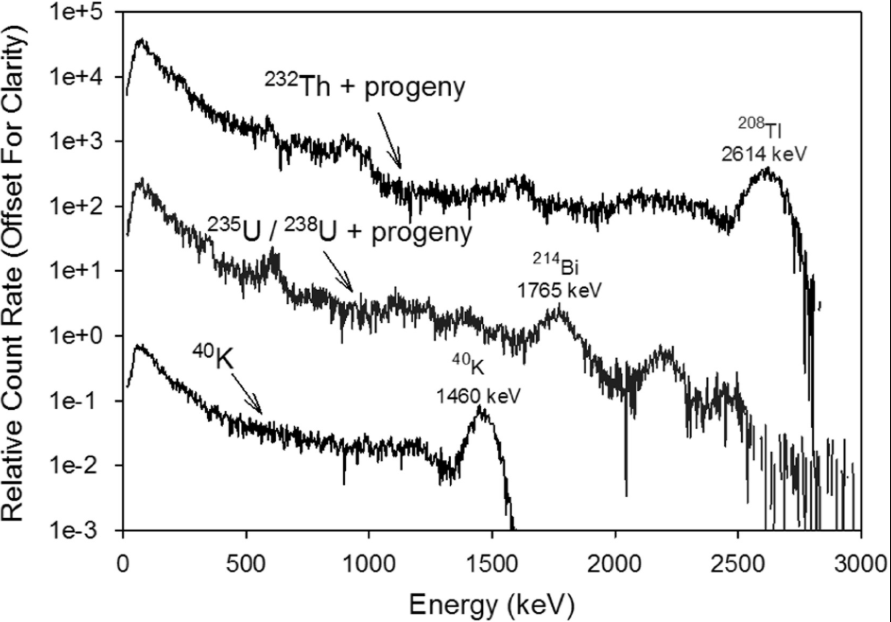
\includegraphics[width=0.8\linewidth]{images/background_components}
\caption{Monte Carlo simulations of background component spectra in NaI(Tl) \cite{KULISEK2015}.}
\label{fig:background_components}
\end{figure}

These radiation components can change both spatially and temporally. Background radiation isotope concentrations change geologically, (Figures \ref{fig:USGS_u_conc}, \ref{fig:USGS_th_conc}, and \ref{fig:USGS_k_conc}) creating different background radiation patterns in different parts of the country. Local changes in soil composition and building materials also are significant enough to change background. Because common building materials like concrete and granite contain radioactive elements, the proximity to these structures cause local variations in background. 

Background also changes over time. This change is largely due to the decay products of $^{222}$Rn gas generated by uranium decay in soil \cite{knoll}. Rain can also increase the level of background radiation by releasing trapped radon gas and other radioactive sources in the soil.

% Air Survey on Background Gradients https://www-sciencedirect-com.proxy2.library.illinois.edu/science/article/pii/S0265931X13002373

\begin{figure}[H]
\centering
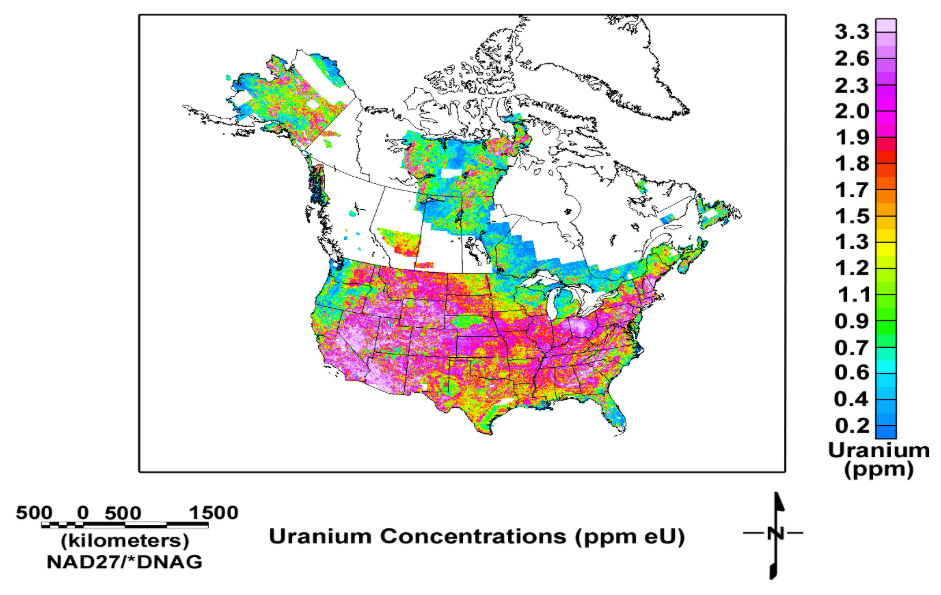
\includegraphics[width=0.9\linewidth]{images/USGS_u_conc}
\caption{Map of uranium concentrations in the United States \cite{USGS}.}
\label{fig:USGS_u_conc}
\end{figure}

\begin{figure}[H]
\centering
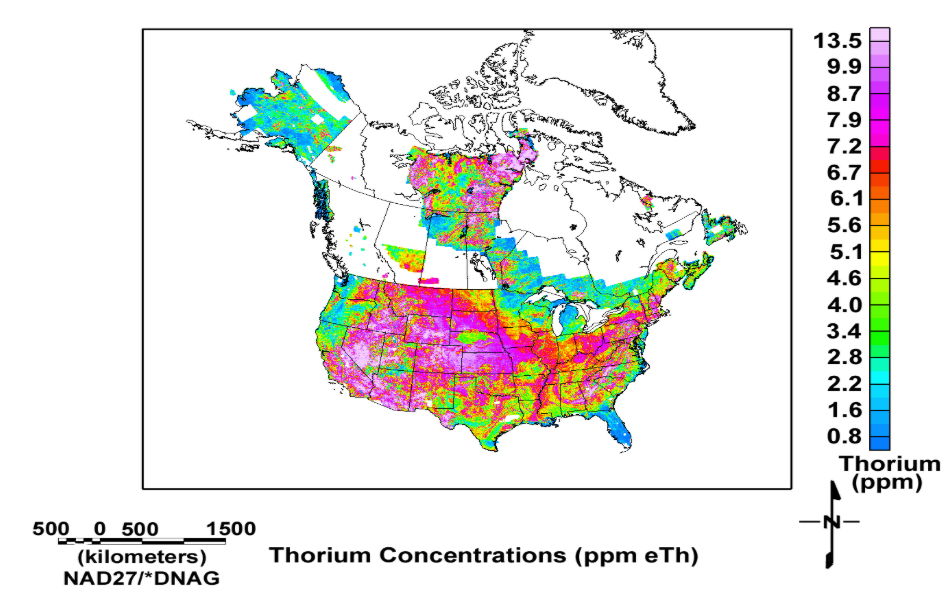
\includegraphics[width=0.9\linewidth]{images/USGS_th_conc}
\caption{Map of thorium concentrations in the United States \cite{USGS}.}
\label{fig:USGS_th_conc}
\end{figure}

\begin{figure}[H]
\centering
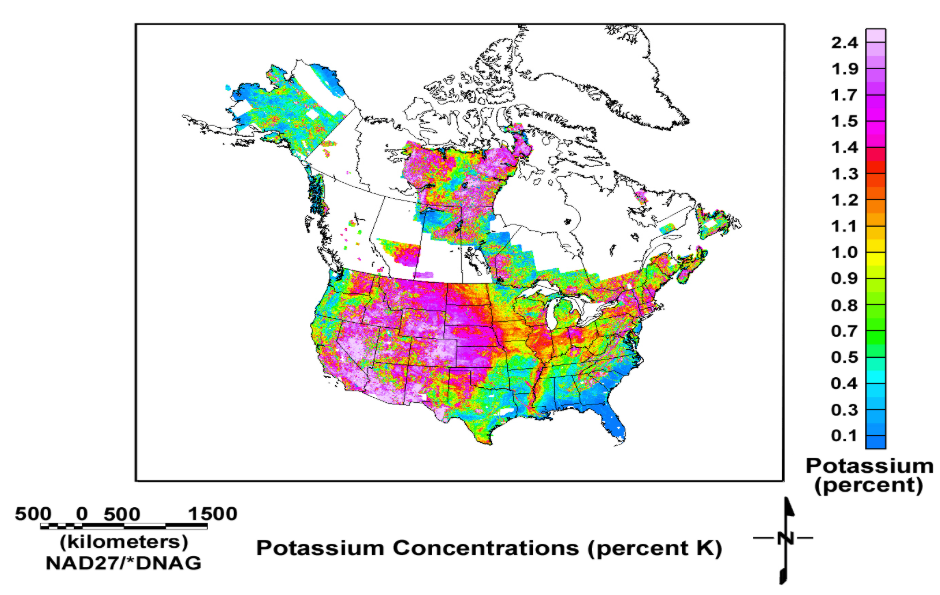
\includegraphics[width=0.9\linewidth]{images/USGS_k_conc}
\caption{Map of $^{40}$K concentrations in the United States \cite{USGS}.}
\label{fig:USGS_k_conc}
\end{figure}

% \USGS Open-File Report 2005-1413: Terrestrial Radioactivity and
%Gamma-ray Exposure in the United States and Canada," 2013.
% [Online]. Available: http://pubs.usgs.gov/of/2005/1413/maps.htm


\subsection{Affect of Temperature on Calibration and Resolution}

% https://www.pnnl.gov/main/publications/external/technical_reports/pnnl-14735.pdf

The calibration of a NaI(Tl) detector can be changed due to drifts in electronics, such as the dynode, and drifts in temperature of the crystal. Calibration drift has been identified as a key factor in the poor performance of RIIDs \cite{blackadar2003}. The dominance of different NaI(Tl) scintillation light decay processes \cite{IANAKIEV2009432} and decay time constants of these processes\cite{MOSZYNSKI2006739} are sensitive to temperature. These factors lead to appreciable changes in relative photopeak position with temperature, shown in Figure \ref{fig:CASANOVAS2012588}, and detector resolution, shown in Figure \ref{fig:temp-dependence-resolution-moszynski}. 

While automated gain stabilization methods exist, many requiring a clear photopeak in the spectrum to calibrate from. This can be achieved by measuring long enough to identify a background photopeak, attaching an external radioactive source to the detector, or by adding a reference light source. Measurement times long enough to identify a background photopeak may be infeasible for certain applications or the calibration step ignored altogether as a part of typical operation. Adding an external source of radiation adds additional noise to the spectrum and additional light sources may malfunction. For these reasons, software-based automated gain stabilization techniques should be used to overcome this issue.

\begin{figure}[H]
\centering
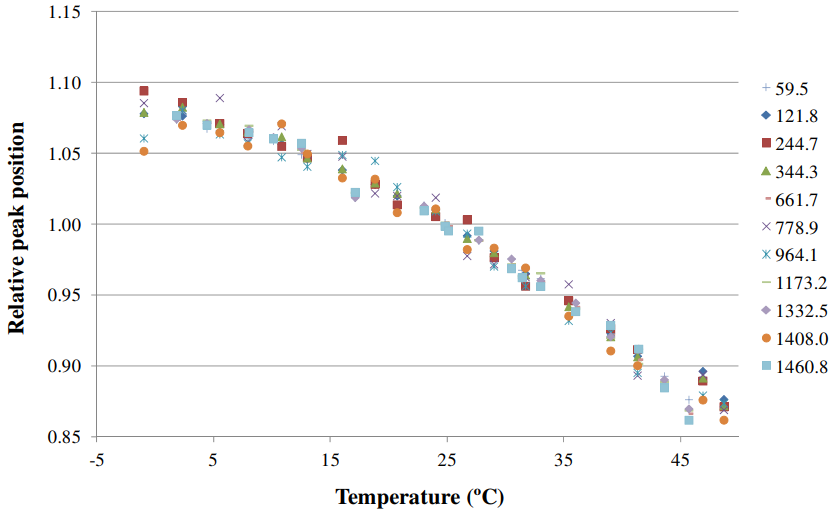
\includegraphics[width=0.95\linewidth]{images/temp_vs_relative_peak_position_CASANOVAS2012588}
\caption{Temperature vs relative photopeak position for an ORTEC Model 905-3 2x2 NaI(Tl) detector.  Reproduced from \cite{CASANOVAS2012588}.}
\label{fig:CASANOVAS2012588}
\end{figure}



\begin{figure}[H]
\centering
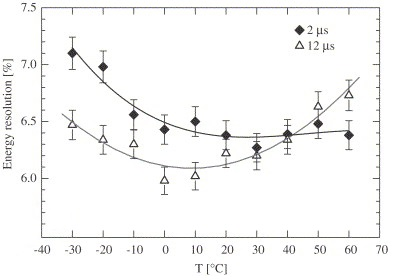
\includegraphics[width=0.95\linewidth]{images/temp-dependence-resolution-moszynski}
\caption{The energy resolution measured for 662 keV γ-rays with a 25mm × 30mm NaI(Tl) crystal at 2 and 12 μs peaking times. Reproduced from \cite{MOSZYNSKI2006739}.}
\label{fig:temp-dependence-resolution-moszynski}
\end{figure}

\section{Machine Learning}

In this section, neural network architectures and parameters that effect training will be described. Models will include dense, convolutional, and autoencoder architectures. 

\subsection{General Neural Network Architecture}

% Node/neruon, get this lingo straight here
An ANN is a mathematical model that attempts to map an arbitrary function from $\mathbb{R}^M$ to $\mathbb{R}^N$, where $M$ and $N$ are positive integers. An ANN accomplishes this by mimicking biological neurons. One example of an ANN architecture is shown in Figure \ref{fig:Network}. This ANN has N neurons in input layer A, J neurons in hidden layer B, and K neurons in output layer C. Each neuron in adjacent layers are connected by weights, represented in Figure \ref{fig:Network} by arrows connecting neurons. 


\begin{figure}[H]
\centering
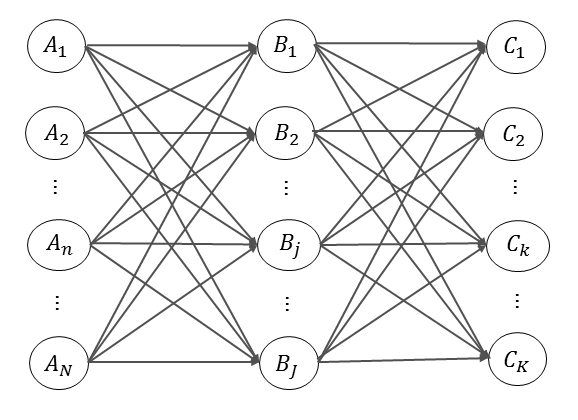
\includegraphics[width=0.75\linewidth]{images/Network}
\caption{Example ANN with input neurons $A_n$, hidden neurons $B_j$, and output neurons $C_k$.}
\label{fig:Network}
\end{figure}


Similar to a biological neuron, the ANN neuron receives input stimuli, performs an operation using it, and outputs the resulting signal. The structure and equation governing the operation of an individual neuron is shown in Figure \ref{fig:Node}. 

\begin{figure}[H]
	\centering
	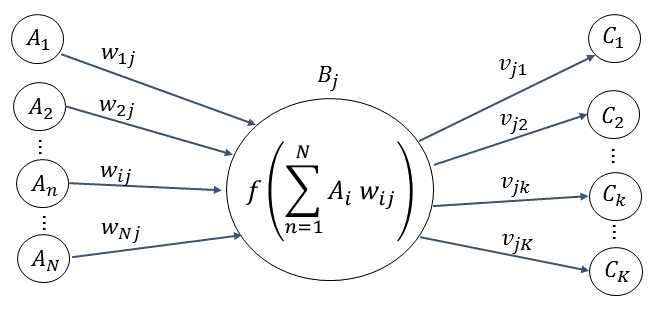
\includegraphics[width=0.75\linewidth]{images/Node_ABC_2}
	\caption{Summary of the operation of a single neuron.}
	\label{fig:Node}
\end{figure}

As seen in Figure \ref{fig:Node}, each neuron operates by summing the products of the previous layers values ($A_1$, $A_2$, ... $A_N$}) and each individual weight ($w_{1j}$, $w_{2j}$, ... $w_{nj}$) connecting the neurons. This summation is analogous to the stimulus a biologic neuron receives from its dendrites. The stimulus is then operated on by an activation function $f$, typically a non-linear function. The output signal is then passed to the next layer of the ANN where the process repeats. An ANN may be trained by setting the network weights, $\mathbf{W}$, in such a way that they minimize the error between target values, $\mathbf{T}$, in a training dataset, $\mathbf{Y}$, and the ANN output given that training dataset, $f( \mathbf{Y} ; \mathbf{W} )$, 
%
\begin{equation} \label{eq:argminW_Error}
\underset{\mathbf{W}}{\text{argmin}} {\text{ Error}}(f(\mathbf{Y} ; \mathbf{W} ) , \mathbf{T} ).
\end{equation}
% \underset{w}{\text{argmin}} \sum_{i=1}^{N} \Vert t_i - y_i \Vert^2
Except under simple cases, Equation \ref{eq:argminW_Error} cannot be solved analytically. Numerical methods for solving this equation include gradient descent through the back-propagation of errors \cite{Rumelhart1986}, genetic learning algorithms \cite{Yao1999}, and Newtons method \cite{Fletcher2000}.


\subsection{Simple Neural Network Example}

An example of a very simple one-layer ANN is shown in Figure \ref{fig:one_layer_net}. This ANN takes two inputs ($x_1$ and $x_2$) and performs the operation shown in Figure \ref{fig:Node}. The weights in the hidden layer connecting the $i^{th}$ input neuron to the $j^{th}$ output neuron will be represented by $w_{ij}$. The bias is set to a constant value of 1. This allows the bias to be effectively trained by changing the weights connecting the bias to the next layer. Using the hyperbolic tangent function, the network outputs for each class $y_1$, $y_2$, and $y_3$ range from -1 to 1. Using these outputs, any input can be classified into a given class if the class' respective output neurons value is above zero, or not in a class if the output neurons value is below zero. The equation for the output of the $j^{th}$ output is given in Equation \ref{eq:single_layer_eq_sum}, where $x_i$ is the $i^{th}$ input from the previous layer, and $b_i$ is the value of the weight connecting the $j^{th}$ output to the bias neuron.
%
\begin{equation} \label{eq:single_layer_eq_sum}
y_j = \tanh(\sum_i x_i w_{ij} + b_j),
\end{equation}

To more clearly understand the geometry of the network's operation, consider the dataset in Figure \ref{fig:training_set_one_layer}. This dataset is composed of three classes: red, green, and blue. The axes that define this dataset are the inputs to the single layer network in Figure \ref{fig:one_layer_net}, ($x_1$,$x_2$). If $\mathbf{W}$ is defined to be a vector with elements ($w_{11}$, $w_{21}$), a line can be defined perpendicular to $\mathbf{W}$ and shifted by $\frac{b_1}{||\mathbf{W}||}$ away from the origin in the direction of $\mathbf{W}$. Given appropriate values for $w_{11}$, $w_{21}$, and $b_1$, a line that separates the blue class from the non-blue class can be created. Any point on the -$\mathbf{W}$ side of the line will have $y_1 < 0$, allowing for classification. Similarly, a separating line for the red class using $w_{12}$, $w_{22}$, and $b_2$ and a separating line for the green class using $w_{13}$, $w_{23}$, and $b_3$ can be constructed. 

The classes in this example dataset are linearly separable, meaning lines can be drawn completely separating each class. If the classes were not linearly separable, additional hidden layers would be necessary to compute the function. It has been shown that additional hidden layers allow the creation of arbitrary decision boundaries \cite{Hornik1991}. 
%
\begin{figure}[H]
	\centering
	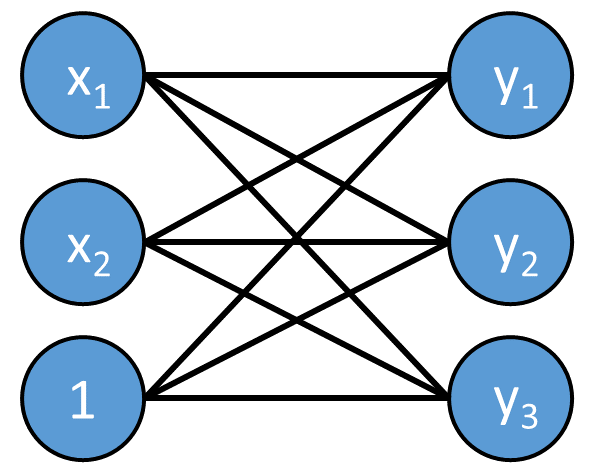
\includegraphics[width=0.45\linewidth]{images/One_layer_net_v31}
	\caption{Example of a single-layer neural network with two inputs ($x_{1}$ and $x_{2}$), three classes ($y_{1}$, $y_{2}$, $y_{3}$), and a bias neuron set to one.}
	\label{fig:one_layer_net}
\end{figure}
% Change these to diff objects to get around grey-scale thesis...?
%The neural network described in Figure \ref{fig:one_layer_net} has two inputs, so its decision boundaries are lines. If the network had three inputs each decision boundary is a plane. Given $N$ inputs, each decision boundary is a $N$-dimensional hyperplane. 


% \cite{Hornik1991} is universal approx theory for ANNs

% pics side by side better? Before and after hyperplane addition?

\begin{figure}[H]
	\centering
	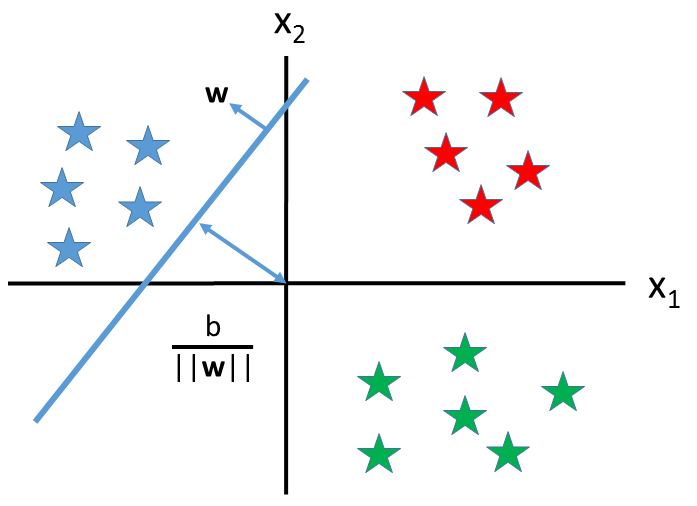
\includegraphics[width=0.65\linewidth]{images/training_set_for_single_layer_hyperplane_v2}
	\caption{One possible dataset describing a three class function. Each class is represented by a different color.}
	\label{fig:training_set_one_layer}
\end{figure}

\subsection{Neural Network Training}

One of the most common methods of training an ANN is through error backpropagation. Error backpropagation is a method to minimizes an error function with respect to the weights connecting neurons as seen in Equation \ref{eq:dMSE}. % If the error function is convex with respect to the network weights, the error with respect to the weights in the network can be minimized using its derivative. THIS IS WRONG. ANN with no hidden layers will have a purely convex error fctn wrt weights, add layers and we get local minima/maxima

Training the simple, one-layer ANN requires finding an expression for \ref{eq:dMSE}. For the following section, let $y_i$ be defined as in Equation \ref{eq:single_layer_eq_sum}, $E_{MSE}$ be defined as the mean squared error function, and training data be defined as in Equation \ref{eq:train_data_D} where $\bold{x_n}$ represents the $n^{th}$ training token and $t_n$ represents the $n^{th}$ binary training target \cite{Nielsen2015}. Note, this derivation would need to be repeated for a different error function. By the chain rule,
%
\begin{equation} \label{eq:dMSE}
\frac{dE_{MSE}}{dw_j} = \frac{dE_{MSE}}{dy_i} \frac{dy_i}{dw_j}.
\end{equation}
%
\begin{equation} \label{eq:train_data_D}
 D={(\boldsymbol{x}_1,t_1), ... ,(\boldsymbol{x}_n,t_n)}
\end{equation}
Equation \ref{eq:dMSE} can be solved by first evaluating $\frac{dE_{MSE}}{dy_i}$,
%
\begin{equation} \label{dE_{MSE}/dy_i}
\frac{dE_{MSE}}{dy_i}  = \frac{d}{dy_i} \sum_i(t_i - y_i)^2
\end{equation}
%
\begin{equation} \label{dE_{MSE}/dy_i}
 = \sum_i  \frac{d}{dy_i} (t_i - y_i)^2
\end{equation}
%
\begin{equation} \label{eq:MSE_deriv}
 =  -2 \sum_i  (t_i - y_i).
\end{equation}
%
Evaluating $\frac{dy_i}{dw_j}$,
%
\begin{equation} \label{dE_{MSE}/dy_i}
\frac{dy_i}{dw_j}  = \frac{d}{dw_j} \tanh( \boldsymbol{w}' \boldsymbol{x}_i + b) 
\end{equation}
%
\begin{equation} \label{dE_{MSE}/dy_i}
 = \tanh'( \boldsymbol{w}' \boldsymbol{x}_i + b) \frac{d}{dw_j}( \boldsymbol{w}' \boldsymbol{x}_i + b)
\end{equation}
%
\begin{equation} \label{dE_{MSE}/dy_i}
 = \tanh'( \boldsymbol{w}' \boldsymbol{x}_i + b)  x_{ij}.
\end{equation}
%
\noindent where $x_{ij}$ is the $j^{th}$ feature of the $i^{th}$ training vector.
%
The update rule for the bias vector is found using
%
\begin{equation} \label{eq:ladidadi}
\frac{dE_{MSE}}{db_j} = \frac{dE_{MSE}}{dy_i} \frac{dy_i}{db_j}.
\end{equation}
%
The expression for $\frac{dE_{MSE}}{dy_i}$ is known from Equation \ref{eq:MSE_deriv}. Evaluating the other derivative in \ref{eq:ladidadi},
%
\begin{equation} \label{dE_{MSE}/dw_j}
\frac{dy_i}{db_j} = \frac{d}{db_j} \tanh(\boldsymbol{w}'\boldsymbol{x}_i + b),
\end{equation}
%
\begin{equation} \label{dE_{MSE}/dy_i}
 = \tanh'( \boldsymbol{w}' \boldsymbol{x}_i + b).
\end{equation}
%
Finally, the gradient of the error function with respect to a single weight can be computed, 
%
\begin{equation} \label{eq:dE_{MSE}/dw_j_final}
\frac{dE_{MSE}}{dw_j} =  -2 \sum_i  (t_i - y_i) \tanh'( \boldsymbol{w}' \boldsymbol{x}_i + b)  x_{ij},
\end{equation}
%
and a single bias,
%
\begin{equation} \label{eq:dE_{MSE}/db_j_final}
\frac{dE_{MSE}}{db_j} =  -2 \sum_i  (t_i - y_i) \tanh'( \boldsymbol{w}' \boldsymbol{x}_i + b).
\end{equation}
%
The derivative in Equations \ref{eq:dE_{MSE}/dw_j_final} and \ref{eq:dE_{MSE}/db_j_final} can used to update each weight and bias in the network as defined by 
%
\begin{equation} \label{eq:update1}
\Delta w_{j} = - \eta \frac{dE_{MSE}}{dw_j}
\end{equation}
%
and 
%
\begin{equation} \label{eq:update2}
\Delta b_{j} = - \eta \frac{dE_{MSE}}{db_j}
\end{equation}
%
where $\eta$ in Equations \ref{eq:update1} and \ref{eq:update2} represents the learning rate of the neural network. The learning rate and its effect on training will be discussed more thoroughly in a later section.

Gradient descent can also be applied to multi-layer ANN. Given an L-layer network where the input stimuli to the $l^{th}$ layer training example x is represented by
%
\begin{equation} \label{eq:CrossEntropy}
\boldsymbol{z}^{x,l} = \boldsymbol{w}^{l}  \boldsymbol{a}^{x,l-1} + \boldsymbol{b}^{l}
\end{equation}
%
where $\boldsymbol{w}^{l}$ is the $l^{th}$ layer's weight matrix, $\boldsymbol{b}^{l}$ is the $l^{th}$ layer's bias vector, and the output activation vector from the $(l-1)^{th}$ layer is 
%
\begin{equation} \label{eq:CrossEntropy}
\boldsymbol{a}^{x,l-1} = f^{l-1}(\boldsymbol{z}^{x,l-1})
\end{equation}
%
where $f^{l-1}$ represents the non-linear activation function used in the $(l-1)^{th}$-layer. Defining the output error as 
%
\begin{equation} \label{eq:CrossEntropy}
\delta^{x,L} = \frac{\partial C}{\partial a^{x,L}} \odot \frac{\partial f^{l-1}(\boldsymbol{z}^{x,l-1}) }{\partial \boldsymbol{z}^{x,l-1}}, 
\end{equation}
%
where $\odot$ is the Hadamard product, the output error can backpropagate to previous layers. For each $l=L-1,L-2,...,2$ an error can be defined by
%
\begin{equation} \label{eq:CrossEntropy}
\delta^{x,l} = ((\boldsymbol{w}^{l+1})^T \delta^{l+1}) \odot \frac{\partial f^{l}(\boldsymbol{z}^{x,l}) }{\partial \boldsymbol{z}^{x,l}}.
\end{equation}
%
The gradient of the cost function as a function of each individual weight and bias can now be defined as 
%
\begin{equation} \label{eq:CrossEntropy1}
\frac{\partial E}{\partial w_{jk}} = a^{l-1}_k \delta^l_j
\end{equation}
%
and 
%
\begin{equation} \label{eq:CrossEntropy2}
\frac{\partial E}{\partial b_j} = \delta^l_j.
\end{equation}
%
Using Equations \ref{eq:update1} and \ref{eq:update2}, the weights can be updated for a single iteration of backpropogation. 

% Other early stopping methods include 


% Where this simple accuracy test is not applicable, such as for regression training sets, a condition based on the ANN training error metric can be used.

ANNs require some stopping condition to conclude training. Stopping conditions include ending training when a threshold in network accuracy on a testing set is reached and ending training when the accuracy has not improved (either by some factor or absolutely) in a fixed number of epochs. Early stopping has the benefit of preventing overfitting and encouraging generalization. Early stopping works by removing a small portion of the training data and defining it as testing data. The ANN is trained using the new training data while some error metric for both the training and testing set are recorded. As training progresses, the ANN likely will overfit to the training data, leading to an increase in error for the testing dataset. Early stopping ends training before overfitting occurs, as illustrated in Figure \ref{fig:training_testing_error}. Because training is stopped before the error in a dataset unknown to the model increases, generalization, or the ability for the ANN to correctly identify patterns outside of the training set, is also improved.

\begin{figure}[H]
	\centering
	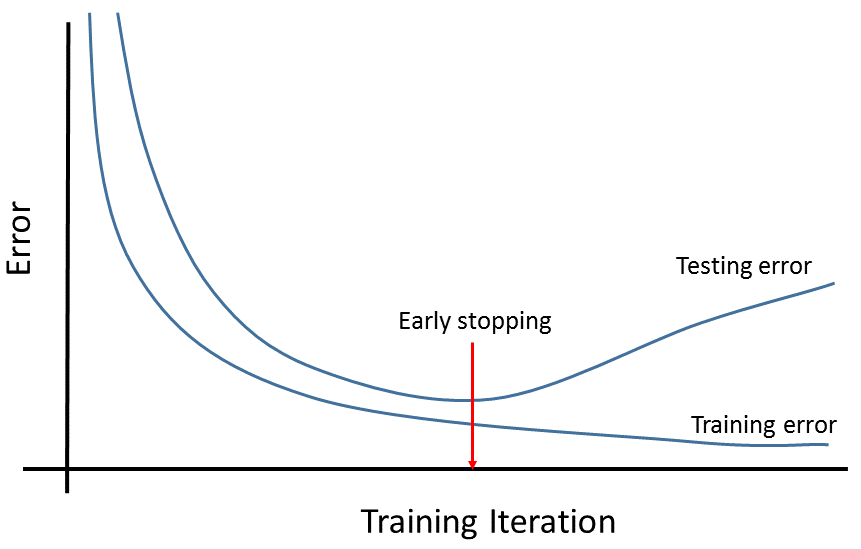
\includegraphics[width=0.85\linewidth]{images/training_testing_error_v2}
	\caption{Ideal training and testing error curves.}
	\label{fig:training_testing_error}
\end{figure}

\subsection{Convolution Neural Networks}

Before the popularization of machine learning, many pattern recognition algorithms relied on hand-crafted feature extractors and a simple trainable classifier like a linear model or naive Bayes. One difficulty in this is the expense in leveraging domain knowledge to design the custom feature extractors. Another challenge comes when the model is applied to a similar but more difficult problem, potentially requiring a new set of feature extractors. While these new features could be based on the old analysis, recreating them would still be costly and require considerable effort.

Deep learning algorithms use a dataset to learn optimum feature extraction and classification techniques simultaneously. CNNs do this by using locally connected convolutional filters instead of fully connected weights. DNNs are fully connected architectures, which means each activation from the previous layer is considered in the next. This leads to redundancy in problems where the input has local structure, like in image recognition or signal processing. Additional CNN layers add hierarchies of representations, meaning that early layers use simple features and deeper layers combine them into more complex features. The magnitude of abstraction can be controlled by tuning the number of convolution layers in a model. Because low-level features are usually shared among the classes in some data (e.g. edge detection in hand-written digits) the convolutional filters can be shared between classes. This weight sharing decreasing the amount of parameters in the model which decreases the probability of overfitting. Weight sharing also makes the model more robust against transformations in the input (e.g. rotations, scaling, and translations).

One of the first CNN architectures was LeNet-5 \cite{Lecun1998}. LeNet-5, shown in Figure \ref{fig:cnn_mnist_lecun98}, classified 32x32 images of handwritten digits using two convolution-average pooling layers followed by two dense layers and an output. This was the first example of a machine learning algorithm creating custom filters and a classification model for the MNIST dataset.

% AlexNet \cite{Krizhevsky2012} was the first exploration into wider and deeper CNNs. 

% Much more work has been done furthering CNNs. VGG \cite{Simonyan2014} showed that smaller filter sizes are good. 

\begin{figure}[H]
	\centering
	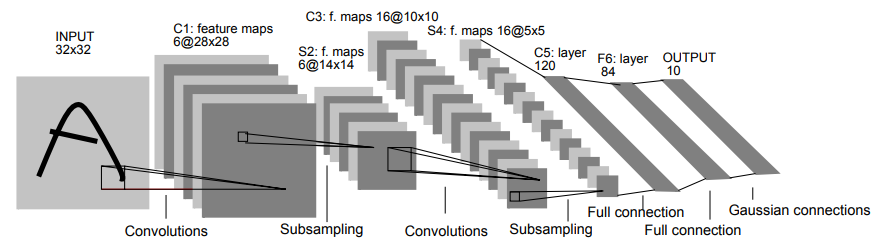
\includegraphics[width=0.85\linewidth]{images/cnn_mnist_lecun98}
	\caption{Architecture of LeNet-5, a CNN created for digit recognition. Image reproduced from \cite{Lecun1998}}
	\label{fig:cnn_mnist_lecun98}
\end{figure}

\section{Autoencoders} \label{Autoencoders}
% \cite{CHARTE2018} is a practical guide to autoencoders. Great resource.

Autoencoders were introduced by Hinton \cite{Hinton2006} as a generalized nonlinear dimension reduction technique. An autoencoder is a neural network designed to learn a compact representation of some input. This is accomplished by simultaneously training an encoding network and a decoding network. An example of this can be seen in Figure \ref{fig:Autoencoder_structure}. The encoding ANN reduces an $n-$dimension input signal, $X$, to a $m-$dimension signal, $z$, where $m < n$. The decoding ANN takes the encoded signal, $z$, and outputs a reproduction of the input signal, $X'$. Once trained, the encoder can be used as a method to pre-train other neural networks or as a feature extractor \cite{CHARTE2018}. 

Methods to encourage the network to learn useful features include forcing the autoencoder to perform denoising \cite{Vincent2008, Vincent2010} and using an undercomplete representation as the encoding layer. Denoising autoencoders corrupt their input with noise, making the autoencoder learn more robust features than those used for simply copying the input. 

% \cite{Masci2011} demonstrated that stacking convolution layers made a good autoencoder.

Other feature extraction methods exist. Principal component analysis (PCA) attempts to reduce the dimensionality of a dataset into linearly uncorrelated variables \cite{Jolliffe2002}. Using a few of these principle components, the data may be represented in a reduced space that contains most of the information present in the original data. Another linear feature extraction method is called linear discriminant analysis (LDA). LDA is a supervised feature extraction method that finds linear combinations of features that can be used to separate classes. Non-linear feature extraction methods, such as kernel PCA, also exist. Kernel PCA applies a non-linear transform to the input space and applies PCA to the data in this transformed space. For kernel PCA to perform well, the correct kernel must be chosen for a given problem, which is a non-trivial task.

% While autoencoders were touched on in the uranium enrichment work, they have not been explored thoroughly. There is some evidence that the autoencoder was overtrained to the A special case of denoising autoencoders will be explored for the ANSI dataset. 



% In addition to using fully connected autoencoders, a 1-D convolutional autoencoder will also be explored. A DNN does not assume the input has local spatial structure, while a CNN does. Because gamma-ray spectra have local spatial structure in the form of photopeaks and Compton continua, it may be better to use a CNN over a DNN \cite{CHARTE2018}. To test this, the experiment described above will be repeated using a 1-D convolutional autoencoder.


\begin{figure}[H]
\centering
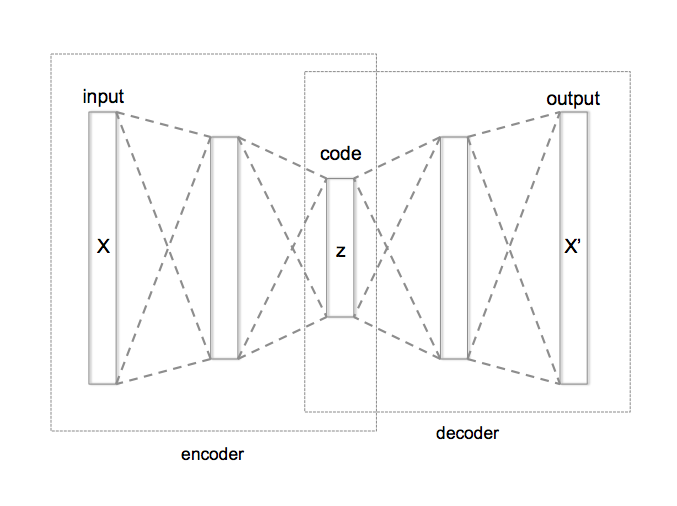
\includegraphics[width=0.8\linewidth]{images/Autoencoder_structure}
\caption{An example of an autoencoder \cite{wiki:AutoencoderStructure}.}
\label{fig:Autoencoder_structure}
\end{figure}


% Fully connected ANNs do not assume there is local spatial structure in a signal, so the fully connected ANN would need to learn that there is local structure. Convolutional ANNs assume there is local structure, and the extent of this structure can be changed by changing the length of the convolutional ANNs filters.

% Once the autoencoder is trained, the hidden layer and output layer (representing the reconstructed spectrum) will be used to train a separate ANN for isotope identification and quantification. The performance of these ANNs will be compared.



\subsection{Hyperparameters}

In addition to the weights connecting neurons, ANNs can have additional hyperparameters. Hyperparameters determine both the networks structure (number of layers, number of nodes in each layer, activation function for each layer) and how the model learns (learning rate, momentum, loss function). In the following section, various hyperparameters and their effects on ANN learning are discussed.

\subsubsection{Learning Rate}

The learning rate is a tunable parameter that affects the magnitude of each weight update. If $\eta$ is too small, the network will learn slowly and training will be inefficient. If $\eta$ is too large, the network will fail to learn, either by converging to a non-extremum or by diverging. An example of a small and large learning rate are shown in Figure \ref{fig:Learning_rate_comparison} 

\begin{figure}[H]
	\centering
	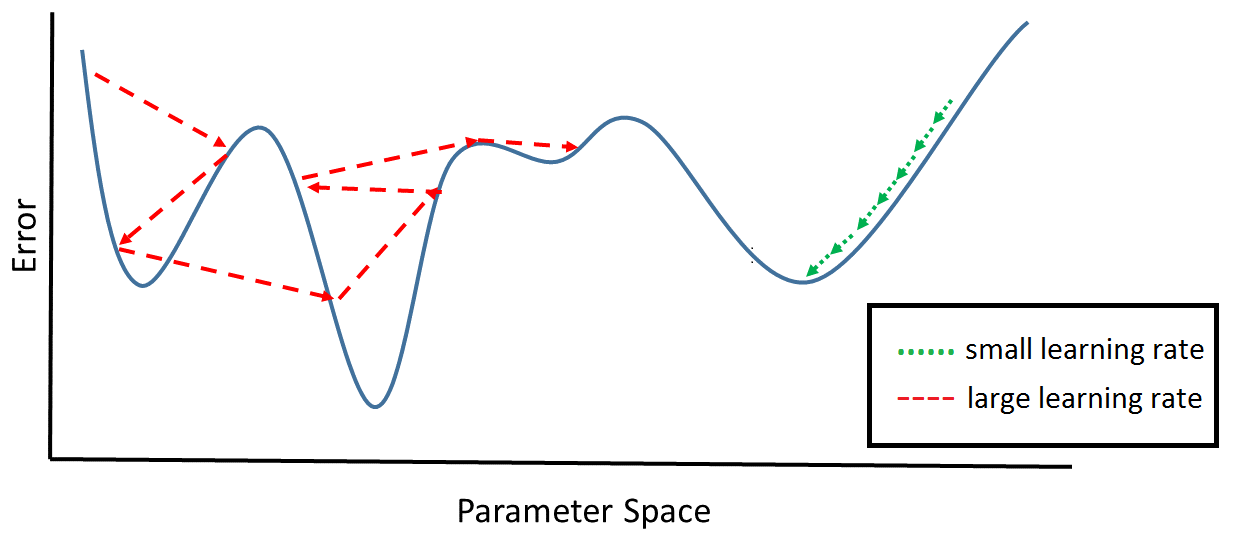
\includegraphics[width=0.8\linewidth]{images/Learning_rate_comparison_v2}
	\caption{Example training paths for a large learning rate, red, and a small learning rate, green.}
	\label{fig:Learning_rate_comparison}
\end{figure}


There are many methods to modify $\eta$ to encourage more efficient learning. One method to increase the speed of learning is to start with a large $\eta$ and decrease $\eta$ as a function of iteration number. Ideally, this method would lead to quick initial learning when far from an optima and slower learning near an optima to more finely explore it. The difficulty with this method is the requirement for a function that slows the learning rate efficiently for a given problem.

\subsubsection{Learning Momentum}

Another method to speed up learning is to add a momentum hyperparameter, $\mu$, to the weight update algorithm \cite{Yu1997}, 
%
\begin{equation} \label{eq:update_momentum}
\Delta w_{ij}(n) = - \eta \frac{dE_{MSE}}{dw_j} +\mu \Delta w_{ij}(n-1).
\end{equation}
%
Similar to the goal of slowing learning over time described above, the momentum term attempts to slow learning near optima. The momentum will be large when the weights are updated at large steps, far from an optima, but will decrease near an optima, allowing slower learning near an optimum.
 
\subsubsection{Training Algorithms}

There are many ANN training algorithms that employ clever learning rate schedules and momentum functions. These algorithms include but are not limited to: Nesterov's accelerated gradient \cite{nesterov1983}, simulated annealing \cite{Kirkpatrick1983}, ADADELTA \cite{ADADELTA}, and ADAM \cite{Kingma2015}. 

The ADAM optimizer was chosen as the training algorithm for the work presented in this thesis due to its incorporation of parts of other successful optimization algorithms and its reported superior performance over these algorithms. Another benefit of the ADAM optimizer is introduction of only one hyperparameter, the learning rate. 

The ADAM optimizer update rule is described below. For the following, $g_t$ is the gradient of the error function with respect to the network parameters at iteration $t$, 
\begin{equation} \label{eq:adam1}
m_t = \beta_1 m_{t-1} + (1 - \beta_1) g_t,
\end{equation}
is the estimate of the mean of the gradient at iteration $t$ and
\begin{equation} \label{eq:adam2}
v_t = \beta_2 v_{t-1} + (1 - \beta_2) g_t^2
\end{equation}
is the estimate of the variance of the gradient at iteration $t$. For the following, the variables $\beta_1$ and $\beta_2$ are parameters called decay rates, $\epsilon$ is another parameter, and $\theta_t$ represents the network parameters at iteration $t$. As described by Kingma and Lei Ba, The default values for $\beta_1$, $\beta_2$, and $\epsilon$ are 0.9, 0.999, and $10^{-8}$ respectively \cite{Kingma2015}. These values were seen to work well for a variety of problems. While these hyperparameters can also be tuned, it has been shown that the default values work well for a variety of network architectures and datasets \cite{Kingma2015}. The bias-corrected first moment estimate is given by
\begin{equation} \label{eq:adam3}
\hat{m}_t = \dfrac{m_t}{1 - \beta^t_1}
\end{equation}
and the bias-corrected second moment estimate is given by 
\begin{equation} \label{eq:adam4}
\hat{v}_t = \dfrac{v_t}{1 - \beta^t_2}.
\end{equation}
Finally, the weight update equation is computed as
\begin{equation} \label{eq:adam5}
\theta_{t+1} = \theta_{t} - \dfrac{\eta}{\sqrt{\hat{v}_t} + \epsilon} \hat{m}_t.
\end{equation}


%Due to the number of free parameters in a ANN (each hidden layer weight is a free parameter), these models have a tendency to overfit data. The three methods used to prevent overfitting in this thesis are $L_2$ regularization, neuron dropout, and data augmentation. These techniques greatly improve the performance of the presented ANN. 

% Is this neccesary? Just mentioning it is enough I think.

%Another method is to randomly perturbing the weights during training using a simulated annealing technique \cite{Kirkpatrick1983}. Simulated annealing mimics how crystal lattices bond together in cooling metal to achieve a low energy state. As metal cools, its crystal lattice will orient itself to lower its total bond energy, but occasionally due to statistical heating sections will jump to a higher energy level. This encourages a global low energy state, as many local low energy state regions are discouraged. This process can be mimicked in a learning algorithm by randomly perturbing the weights during learning. As learning continues the network 'cools' and the frequency of weight perturbation decreases. It can be shown that given a long enough annealing schedule, the global optimum solution for a problem is guaranteed to be found \cite{Granville1994}.

\subsubsection{Cost Function}

The choice of cost function to train against depends on the targets the network is attempting to learn. One of the simplest error functions is the binary accuracy for classification, 
%
\begin{equation} \label{eq:Binary_accuracy}
E_{Binary} = {\frac{1} N} \sum_{n=1}^N [\hat{y}_n \neq y_n ],
\end{equation}
%
where N is the total number of output neurons, $y_n$ is the ground truth of the n$^{th}$ output, and $\hat{y}_n$ is the ANN output of the n$^{th}$ output neuron. While this is a simple function, it penalizes the model for being close to the answer. Because there is no incremental indication that a model is improving, this error function is not typically used for gradient descent algorithms.

A simple differentiable cost function is the mean squared error (MSE) function shown in Equation \ref{eq:MSE_error}. This function is differentiable, so gradient descent algorithms can be applied to it. The MSE function is appropriate when targets are any real number, as in a regression problem. 
%
\begin{equation} \label{eq:MSE_error}
E_{Binary} = {\frac{1} N} \sum_{n=1}^N (\hat{y}_n - y_n)^2,
\end{equation}
%
For classification problems, the average cross entropy, shown in Equation \ref{eq:CrossEntropy} can be used. Cross entropy measures how different the probability distributions $y_n$ and $\hat{y}_n$ are from each other. Because the cross entropy treats $y_n$ and $\hat{y}_n$ as probability distributions, they are required to exist in the range [0,1].
%
\begin{equation} \label{eq:CrossEntropy}
E = -{\frac{1} N} \sum_{n=1}^N y_n \log(\hat{y}_n) +  (1-y_n) \log(1-\hat{y}_n), 
\end{equation}
%

Because the softmax function can be used for classification, it is traditionally used as the output function for the model when using the cross entropy cost function. The softmax function is used in binary classification problems to calculate posterior class probabilities \cite{Bridle1990}.

\begin{equation} \label{eq:softmax}
softmax(z_j) = \frac{\exp(z_j)} {\sum_{k=1}^{K} \exp(z_k)}.
\end{equation}


%% This part is kinda total butts
%It is important to note that for a single layer neural network with the MSE cost function, the one minimum in $MSE(W)$ is the global minimum. When the number of layers increases beyond one there may be many more local minima in the cost function. Care must be taken when training a neural network to either find the global minimum in the cost function with respect to the weights or to find a minimum that reduces the error below a desired value. Care must also be taken to avoid stuck training, or having the optimization algorithm find a local minimum and not move from it. A proper optimization technique must account for these pitfalls. 

\subsubsection{Weight Regularization}

Weight regularization is a hyperparameter that penalizes the ANN when the magnitude of the weights increases. Because the magnitude of the weights is tied to the complexity of the model, adding weight regularization attempts to limit complexity and the probability of overfitting.

A common method of incorporating weight regularization is by adding an $L_n$ regularization term to the error function, as seen in Equation \ref{eq:L2_Reg}. Common values for $n$ are 1 and 2. Adding weight regularization allows the magnitude of the weights to increase only when there is a comparable reduction in the unmodified error function.
%
\begin{equation} \label{eq:L2_Reg}
\tilde{E} = E + \sum_i \lambda w_i^n.
\end{equation}
%
In Equation \ref{eq:L2_Reg}, $w_i$ is the weight between each neuron in the ANN and $\lambda$ is the regularization strength hyperparameter. A larger $\lambda$ will force the ANN to prefer smaller weights connecting the neurons. If the parameter $\lambda$ is too small, the unbounded model complexity may fit only the training data. If the parameter $\lambda$ is too large, the ANN will only minimize the $L_n$ error, failing to learn.

\subsubsection{Neuron Dropout}

Another method to reduce model complexity is neuron dropout. Neuron dropout is the process of temporarily removing a neuron from the ANN architecture \cite{Srivastava2014}. By randomly removing neurons from an ANN during training, heavy local codependency between neurons that could lead to the ANN becoming stuck in a local minimum in the error function, and thus overtraining, is discouraged. The frequency with which neurons are removed is called the neuron dropout rate, which is a hyperparameter.

Almost always, taking the average output of more than one separately trained ANN improves the performance of the ANN \cite{Srivastava2014}. By applying dropout at each neuron with the same probability throughout training, the ANN's architecture changes every iteration. The makes neuron dropout a cost efficient way to effectively average many different ANN architectures, improving performance.

\subsubsection{Data Augmentation}

Data augmentation changes the data during training using physically realistic transformations. For example, a training dataset of images can be rotated, flipped, blurred, or color augmented during training. An example of horizontal flip and a blur augmentation are seen in Figure \ref{fig:cat}. This cheaply expands the training dataset and discourages overtraining, as the ANN never observes the exact same image. Both the augmentation method and strength of said method are hyperparameters. 

\begin{figure}[H]
	\centering
	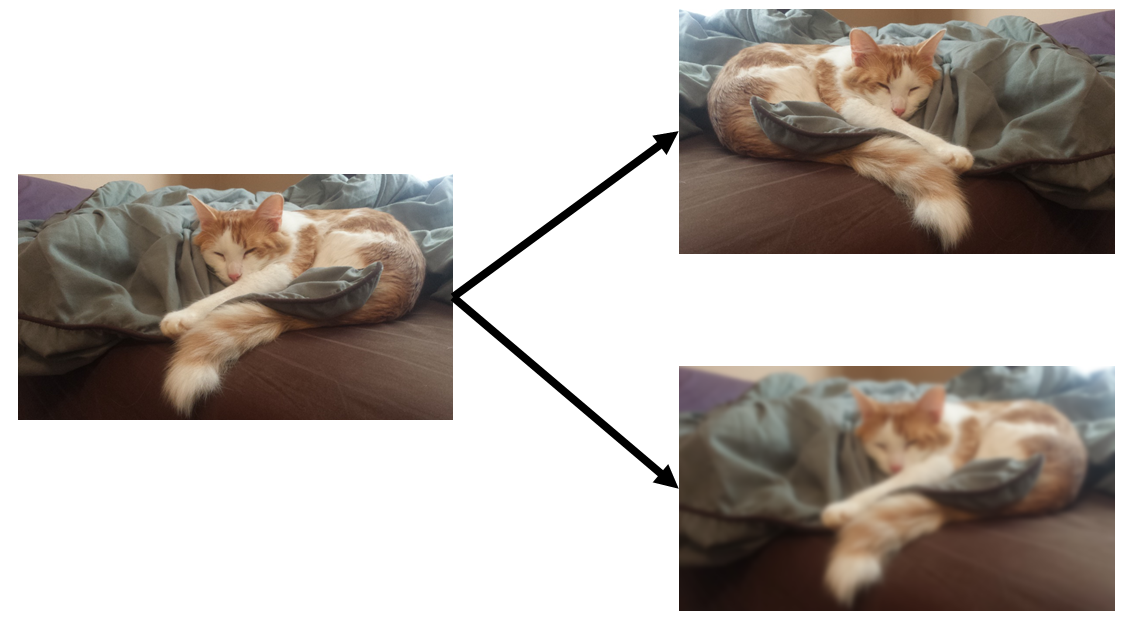
\includegraphics[width=0.9\linewidth]{images/cat}
	\caption{Two examples of data augmentation using an image of a cat. The image to the left is the original. The top right image is augmented using a horizontal flip. The bottom right image is augmented using blur.}
	\label{fig:cat}
\end{figure}

\subsection{Hyperparameter Optimization}

In general, ANNs have many hyperparameters that require optimization. Optimizing these hyperparameters will lead to more efficient training and more accurate performance when training is concluded. There are several different methods to perform hyperparameter optimization for an ANN. These methods may include manual optimization, exhaustive grid search, and random parameter search.

Manually optimizing parameters is necessary when developing a novel algorithm. This involves changing hyperparameters and observing how the ANN trains and the final error on a validation dataset. Ideally, the ANN should train quickly and have a low error on a validation dataset. For many parameters `rule of thumb' values exist that can be used to find parameters that work to some degree. Due to the large hyperparameter space, a manual search is cost prohibitive if further optimization is desired.

Once a range of parameters is determined through a manual search, multiple methods are available to explore the parameter space for an optimal solution. One method is an exhaustive grid search. In a grid search the parameter space is divided into a uniform grid and the joint performance of all parameters is tested. The grid search method is ineffective for two reasons. First, neural networks may have a large number of hyperparameters that need to be explored, and the computational requirement to explore the hyperparameter space increases exponentially with increasing hyperparamters. Second, in practice only a few hyperparameters dominate performance, but the dominating hyperparameters are different for different applications. A grid search may under represent the importance of key hyperparamters, as seen in Figure \ref{fig:Bergstra12a_hyperparameter_grid_vs_random}.  While this method works, it has been shown that a random search in the hyperparameter target domain finds better hyperparameters quicker than testing equally distributed points in the chosen range \cite{Bergstra2012}. It can also be shown that given 60 random samples over some space with a finite minimum, the minimum of those 60 random samples is within 5\% of the true minimum with 95\% probability \cite{Zheng2015}. This means that given a range of hyperparameters, the best performing hyperparameter combination out of 60 randomly sampled points is very likely to be close to optimal. 

\begin{figure}[H]
	\centering
	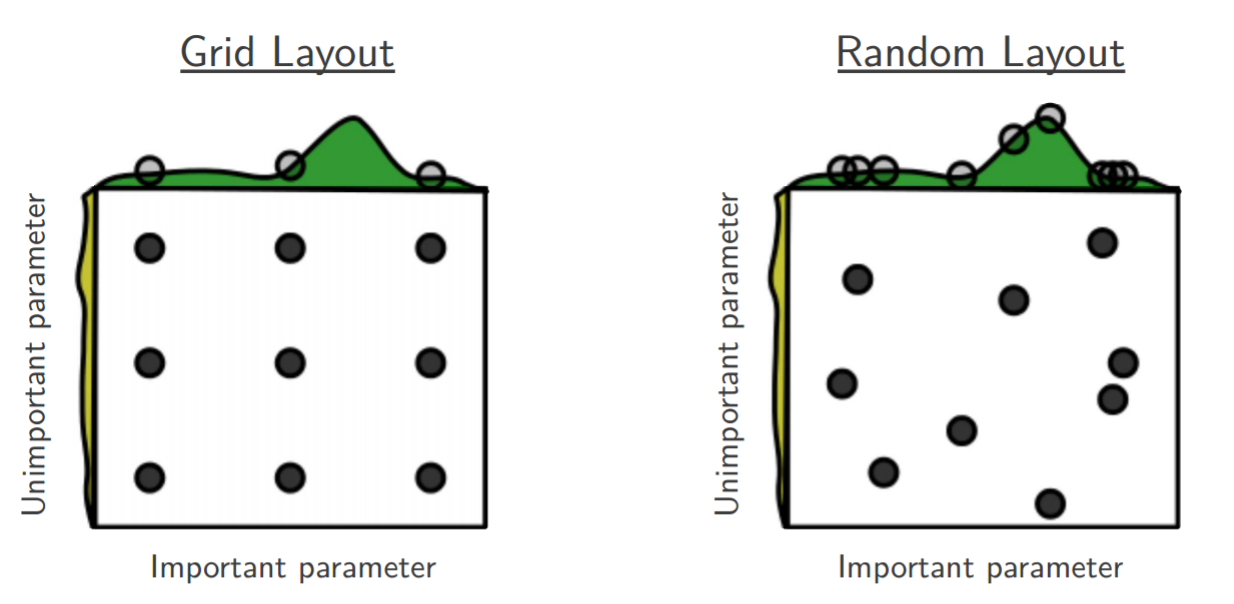
\includegraphics[width=0.99\linewidth]{images/Bergstra12a_hyperparameter_grid_vs_random}
	\caption{A comparison between a grid search and a random search for hyperparameter optimization when performance is strongly tied to one hyperparameter. The green function represents the effect of an important hyperparameter on a cost function while the yellow function represents the effect for an unimportant hyperparameter. Figure reproduced from [42].}
	\label{fig:Bergstra12a_hyperparameter_grid_vs_random}
\end{figure}


The ability for an ANN to solve a problem depends on the network structure, teaching method, and the training set to be learned. In the following section, a method for generating a training set for isotope identification and quantification is described.

To analyze the performance of a random search, a random hyperparameter efficiency curve, example shown in Figure \ref{fig:Bergstra_random_efficiency_curve_DNN} can be used. In the figure, 256 hyperparameter searches are run. These trials are split into experiments with sizes of increasing powers of two. The best performing trial from each experiment is determined and shown using a box plot.


\begin{figure}[H]
	\centering
	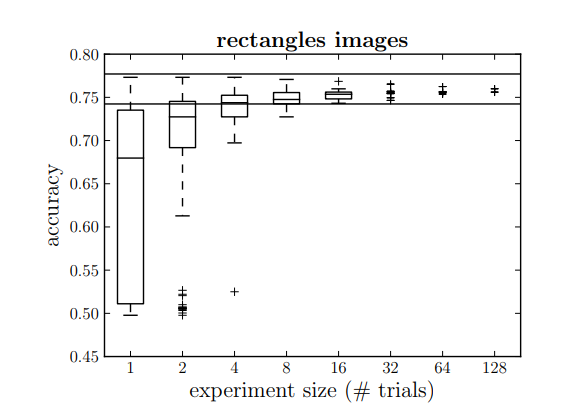
\includegraphics[width=0.9\linewidth]{model_choice_hyperparameter_search_images/Bergstra12_random_efficiency_curve}
	\caption{Example Random efficiency curves for a neural network \cite{Bergstra2012}.}
	\label{fig:Bergstra_random_efficiency_curve_DNN}
\end{figure}



\section{Summary}

In this chapter, the structure of multi-layer ANNs, methods to train and optimize them, and a method to create a training set for isotope identification and quantification have been described. In the following section an ANN will be presented using these concepts and its performance on a number of real and simulated spectra will be discussed. 













\chapter{Machine Learning Models Explored} \label{ChapterMachineLearningModelsExplored}

In this chapter, we investigate which parameters affect the convolutional and dense models' performance for datasets of different complexity. Analyzing which hyperparameters most influence performance informs future research into applying machine learning to gamma-ray spectroscopy. To accomplish this, we ran hyperparameter searches using two datasets: a complete dataset with a wide range of simulated parameters and a simple dataset with smaller parameter ranges. This section describes these datasets and the architectural and regularization hyperparameters choices for the dense and convolutional models. This section concludes with a discussion on the insights obtained from the hyperparameter searches.


% Dense and convolutional models are explored for two different reasons. 

\section{Training Templates Overview}

The datasets used to train the models are created using templates of simulated gamma-ray spectra without Poisson noise. A one-dimensional particle transport code developed at Sandia National Laboratory, GADRAS-DRF (Gamma Detector Response and Analysis Software - Detector Response Function) \cite{mitchell2014}, was used to generate these templates. This simulation code is used to model a radiation detector's response considering environmental scattering and a specific  detector's properties. The GADRAS-DRF interface in Figure \ref{fig:gadras_parameters} shows the detector parameters used in this work. These parameters are from an Ortec 905-3 NaI(Tl) detector included in the Department of Homeland Security's Algorithm Improvement Program (AIP) software package \cite{DHSAIP}. To simulate our template spectra, the detector model's default energy calibration was modified so the detector measured energies from 0 MeV to 3.5 MeV. This was accomplished by setting the calibration offset (Order 0 in E) to zero and the calibration's gain (Order 1 in E) to 3500. The default number of channels was also changed to 1194, calibrating the 1024$^{th}$ channel - the default spectrum length used in this work - to an energy of 3 MeV. This ensures that isotopic signatures higher than 3 MeV are included in the training dataset when a template's calibration is modified to include these energies.

\begin{figure}[H]
	\centering
	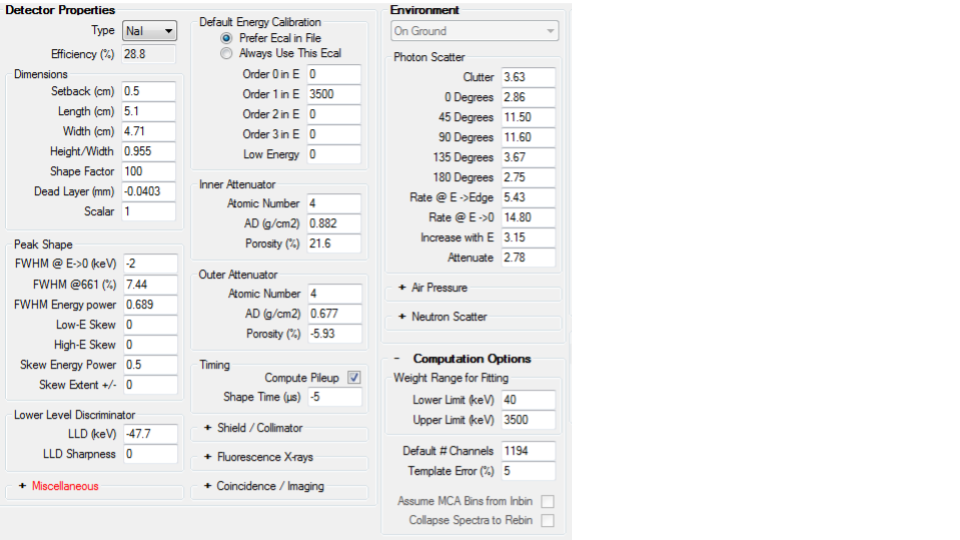
\includegraphics[trim=0 0 390 0,clip,width=0.7\linewidth]{images/gadras_parameters}
	\caption{GADRAS-DRF GUI showing parameters used to simulate the Ortec 905-3 2x2-in NaI(Tl) detector used in this work.}
	\label{fig:gadras_parameters}
\end{figure}


GADRAS-DRF was also used to simulate spectral changes associated with measurement geometry. The measurement scenario used by GADRAS-DRF is illustrated in Figure \ref{fig:gadras_measurement_setup}. Using GADRAS-DRF, we can simulate changes in source-detector distance, the source and detector's mutual height from the ground, and optional shielding material between the source and detector. To demonstrate two of these effects, $^{60}$Co spectra were simulated at various source-detector distances, Figure \ref{fig:sim_spectra_distance_comparison}, and heights above the ground, Figure \ref{fig:sim_spectra_height_comparison}. These parameters change the Compton continuum's shape, the peak-to-total ratio, and the backscatter peak's magnitude. Another parameter that changes the spectrum is the Gaussian energy broadening of the photopeaks. Due to manufacturing differences, each detector has a different amount of energy broadening. Examples of $^{60}$Co spectra with different FWHM parameters are shown in Figure \ref{fig:sim_spectra_FWHM_comparison}.


\begin{figure}[H]
	\centering
	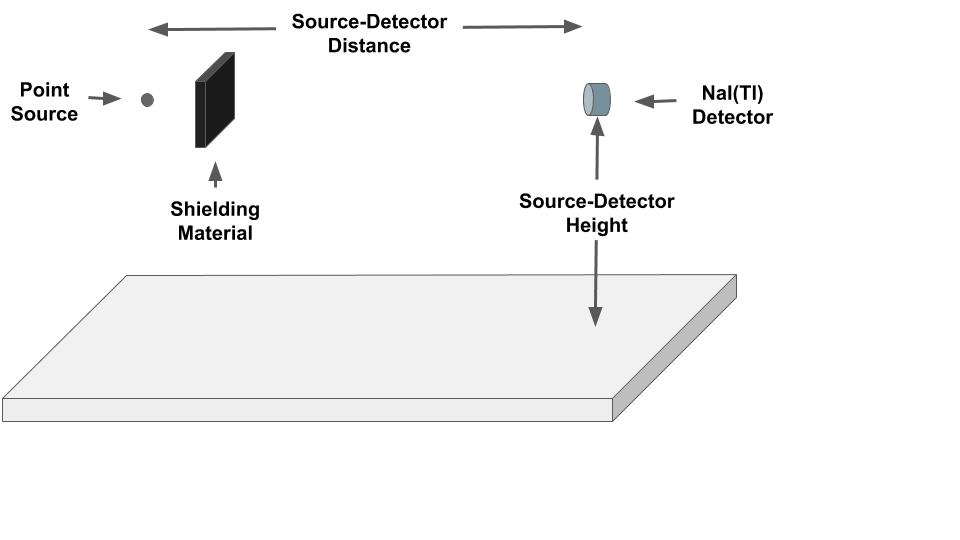
\includegraphics[trim=0 0 180 0,clip,width=0.9\linewidth]{images/gadras_measurement_setup}
	\caption{GADRAS-DRF measurement diagram. Environmental scatter is approximated using the photon scatter terms from Figure \ref{fig:gadras_parameters}.}
	\label{fig:gadras_measurement_setup}
\end{figure}



\begin{figure}[H]
\centering
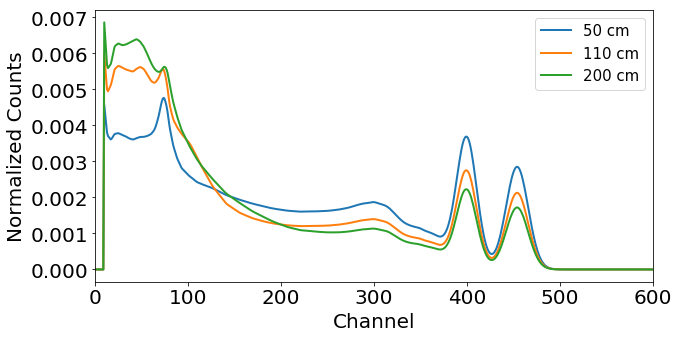
\includegraphics[width=0.75\linewidth]{images/sim_spectra_distance_comparison}
\caption{Comparison of a $^{60}$Co spectrum simulated using various source-detector distances.}
\label{fig:sim_spectra_distance_comparison}
\end{figure}

\begin{figure}[H]
\centering
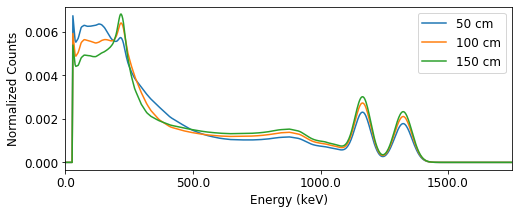
\includegraphics[width=0.75\linewidth]{images/sim_spectra_height_comparison}
\caption{Comparison of a $^{60}$Co spectrum simulated using various source-detector heights off the ground.}
\label{fig:sim_spectra_height_comparison}
\end{figure}


\begin{figure}[H]
\centering
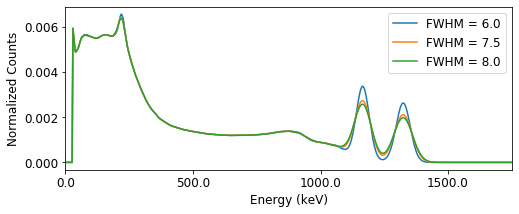
\includegraphics[width=0.75\linewidth]{images/sim_spectra_FWHM_comparison}
\caption{Comparison of a $^{60}$Co spectrum simulated with various FWHM parameters.}
\label{fig:sim_spectra_FWHM_comparison}
\end{figure}




% To incorporate these changes, templates simulated at different distances are included in the dataset. These distances start at 30cm, which is the distance at which a 1 uCi source will have an activity of about 400 cps on a 2 inch diameter detector. This is about twice the expected activity of background. 

% Changes in calibration due to temperature shifts are also considered. Due to the relatively large magnitude in calibration shifts due to temperature shifts from -5 C to 40 C \cite{CASANOVAS2012588}, it is expected incorporating these additions will also make the algorithm robust against calibration.

The template parameters used in this study are shown in Table \ref{table:all_fixed_simulation_parameters}. These parameters are based on handheld RIID scenarios. The source-detector height off the ground are sampled between shin and arm heights (50 cm to 150 cm). The source-detector distance range corresponds to standoff distances expected when measuring a source in a cargo container. The areal density of each material corresponds to 20$\%$, 40$\%$, 60$\%$, and 80$\%$ attenuation of a 200 keV photon. This photon energy was chosen because it is near the 186 keV energy of the characteristic $^{235}$U photopeak. A set of unshielded templates is also included. The FWHM range was chosen based on reported FWHM values for a NaI(Tl) detector (see section \ref{subsection_energy_resolution}). Background locations were chosen based on their geographic and geologic differences.

\begin{table}[H]
	\centering
	\caption{Fixed GADRAS-DRF template simulation parameters.}
	\begin{tabular}{ll}
		\hline
		\textbf{Simulation Parameter} & \textbf{Values} \\ \hline
		Source-detector height [cm] & 50, 100, 125 \\ 
		Source-detector distance [cm] & 50, 175, 300 \\ 
		Areal density of solid aluminum [$\frac{\text{g}}{\text{cm}^{2}}$] & 1.82, 4.18, 7.49, 13.16 \\ 
		Areal density of solid iron [$\frac{\text{g}}{\text{cm}^{2}}$] & 1.53, 3.5, 6.28, 11.02 \\ 
		Areal density of solid lead [$\frac{\text{g}}{\text{cm}^{2}}$] & 0.22, 0.51, 0.92, 1.61 \\ 
		FWHM at  662 keV [\%] & 7.0, 7.5, 8.0 \\ 
		Background Location & \begin{tabular}[l]{@{}l@{}}Albuquerque, Atlanta, Austin,\\ Chicago , Knoxville , Miami\end{tabular} \\ \hline
	\end{tabular}
	\label{table:all_fixed_simulation_parameters}
\end{table}

In addition to the parameters simulated by GADRAS-DRF, parameters are included to perform additional data augmentation. These parameters are shown in Table \ref{table:all_variable_simulation_parameters}.

\begin{table}[H]
\centering
\caption{Default data augmentation parameters.}
\begin{tabular}{l}
\hline
\textbf{Simulation Parameter} \\ \hline
integration time \\ 
background counts per second \\ 
Signal to Background ratio \\ 
Calibration - Offset \\ 
Calibration - Gain \\ \hline
\end{tabular}
\label{table:all_variable_simulation_parameters}
\end{table}

\section{Hyperparameter Search}

To determine which parameters affect the convolutional and dense model's performance on datasets of increasing complexity, hyperparameter searches for each model are performed for a simple and more complicated dataset. The hyperparameter search for a single model and dataset is illustrated in Figure \ref{fig:hyperparameter_search_workflow}. For each dataset and model, 5-folds cross validation is performed on 256 sets of randomly chosen hyperparameters. The maximum number of epochs was set to 200 and an early stopping patience of 20 epochs was used to stop training with the validation dataset's F1 score. In addition to this, training was ended after 10 epochs if the validation dataset's F1 score did cross a 10\% threshold. The hyperparameter combination with the lowest average validation dataset F1 score was declared the optimum hyperparameter combination for that model. The validation dataset being used to end training induces a bias into the score used to determine the best hyperparameter combination. To remove this bias, a separate testing dataset's F1 score would need to be used to determine the optimum hyperparameter combination.

\begin{figure}[H]
	\centering
	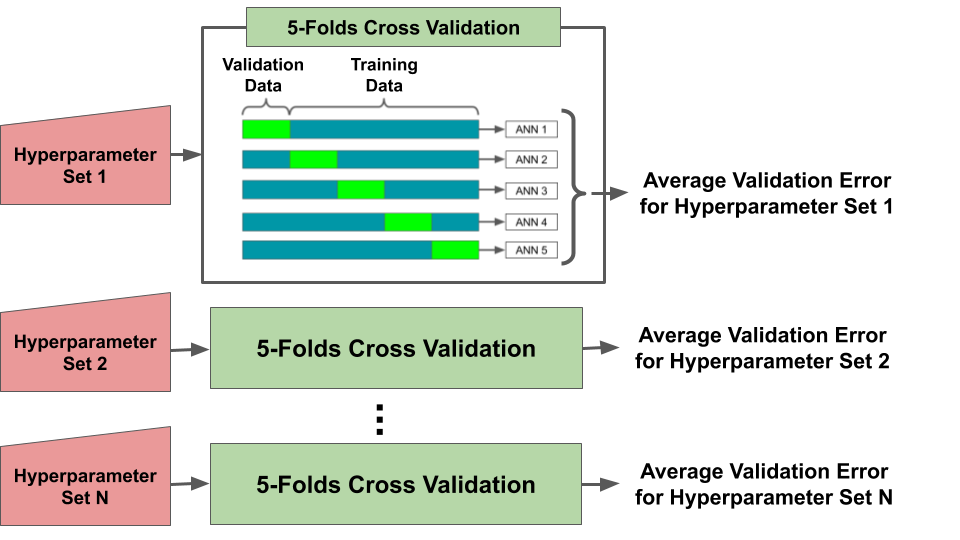
\includegraphics[trim=0 0 40 0,clip,width=1.0\linewidth]{images/hyperparameter_search_workflow}
	\caption{Hyperparameter search workflow.}
	\label{fig:hyperparameter_search_workflow}
\end{figure}


\section{Datasets Used for the Hyperparameter Search} \label{datasets_used_hyperparam_search}

The parameters used for the simple dataset are shown in Table \ref{table:hyperparameter_dataset_easy_parameters} and parameters used for the complete dataset are shown in Table \ref{table:hyperparameter_dataset_full_parameters}. Datasets are simulated using the process described in Section \ref{section_dataset_gen}. Isotopes included in the dataset are from the  ANSI N42-34-2006 standard for isotope identification devices \cite{ANSI}: $^{241}$Am, $^{133}$Ba, $^{57}$Co, $^{60}$Co, $^{51}$Cr, $^{137}$Cs, $^{152}$Eu, $^{67}$Ga, $^{123}$I, $^{125}$I, $^{131}$I, $^{111}$In, $^{192}$Ir, $^{177m}$Lu, $^{99}$Mo, $^{237}$Np, $^{103}$Pd, $^{239}$Pu, $^{240}$Pu, $^{226}$Ra, $^{75}$Se, $^{153}$Sm, $^{99m}$Tc, $^{201}$Tl, $^{204}$Tl, $^{233}$U, $^{235}$U, $^{238}$U, and $^{133}$Xe. In each dataset, a total of 100 spectra were simulated for each isotope. Each dataset also included 100 spectra of only background.

\begin{table}[H]
	\centering
	\caption{Range of parameters used for the simple dataset.}
	\label{table:hyperparameter_dataset_easy_parameters}
	\begin{tabular}{lll}
		\hline
		\textbf{Simulation Parameter} & \textbf{Parameter Range} & \textbf{Sampling} \\ \hline
		Source-Detector Distance [cm] & 175 & N/A \\ 
		Source-Detector Height [cm] & 100 & N/A \\ 
		FWHM at 662 keV & 7.5 & N/A \\ 
		Shielding [\% 200 keV Attenuated] & 0\%, 20\% & Uniform \\ 
		Integration Time [s] & 60 - 600 & Log-Uniform \\ 
		Calibration - Offset [channels] & 0 - 10 & Uniform \\ 
		Calibration - Gain & 0.9 - 1.1 & Uniform \\ 
		Signal to Background Ratio & 0.5 - 2.0 & Uniform \\ 
		Background Counts Per Second & 200 & Poisson \\ \hline
	\end{tabular}
\end{table}


\begin{table}[H]
	\centering
	\caption{Range of parameters used for the complete dataset.}
	\label{table:hyperparameter_dataset_full_parameters}
	\begin{tabular}{lll}
		\hline
		\textbf{Simulation Parameter} & \textbf{Parameter Range} & \textbf{Sampling} \\ \hline
		Source-Detector Distance {[}cm{]} & 50, 175, 300 & Uniform \\ 
		Source-Detector Height {[}cm{]} & 50, 100, 150 & Uniform \\ 
		FWHM 662 keV {[}s{]} & 7.0, 7.5, 8.0 & Uniform \\ 
		Shielding [\% 200 keV Attenuated] & 0\%, 20\%, 40\%, 60\% & Uniform \\ 
		Integration Time {[}s{]} & 10 - 3600 & Log-Uniform \\ 
		Calibration - Offset (channels) & 0 - 10 & Uniform \\ 
		Calibration - Gain & 0.8 - 1.2 & Uniform \\ 
		Signal to Background Ratio & 0.1 - 3.0 & Uniform \\ 
		Background Counts Per Second & 200 & Poisson \\ \hline
	\end{tabular}
\end{table}


The hyperparameter search for a single model and dataset is illustrated in Figure \ref{fig:hyperparameter_search_workflow}. For each dataset and model, 5-folds cross validation is performed on 256 sets of randomly chosen hyperparameters. The maximum number of epochs was set to 200 and an early stopping patience of 20 epochs was used to stop training using the validation dataset's F1 score,
%
\begin{align} \label{eq:f1_score}
\text{F1 score} &= 2 \frac{\text{precision} \cdot \text{recall}}{\text{precision + recall}}
\intertext{where} 
\text{precision} &= \frac{\text{true positives}}{\text{true positives + false positives}} \nonumber \\
\text{recall} &= \frac{\text{true positives}}{\text{true positives + false negatives}}. \nonumber
\end{align}
%
In addition to this, training was ended after 10 epochs if the validation dataset's F1 score did cross a 10\% threshold. The hyperparameter combination with the lowest average validation dataset F1 score was declared the optimum hyperparameter combination for that model. The validation dataset being used to end training induces a bias into the score used to determine the best hyperparameter combination. A better approach would be to use a separate simulated dataset's F1 score to determine the optimum hyperparameter combination.

\begin{figure}[H]
	\centering
	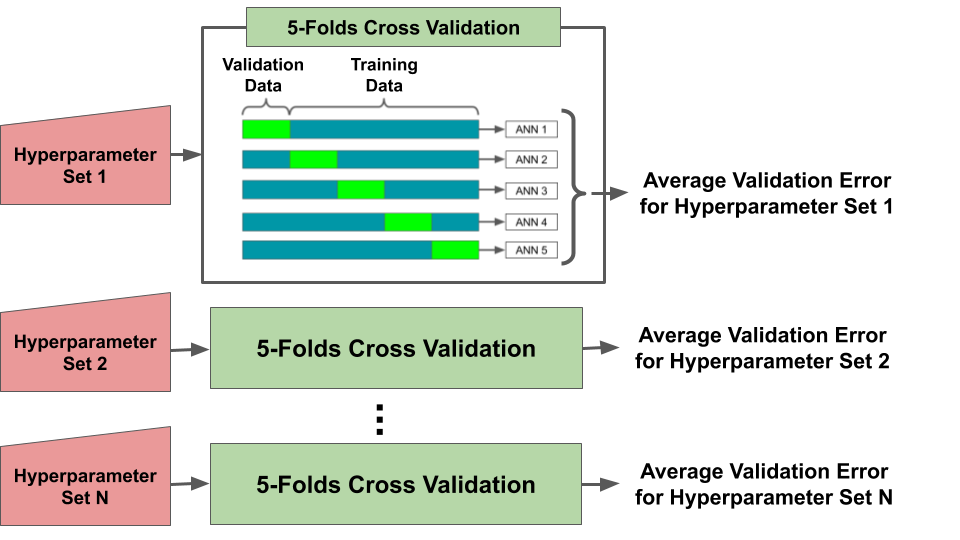
\includegraphics[trim=0 0 40 0,clip,width=1.0\linewidth]{images/hyperparameter_search_workflow}
	\caption{Hyperparameter search workflow.}
	\label{fig:hyperparameter_search_workflow}
\end{figure}

\section{Hyperparameter Search Results}

In this section, hyperparameter search results are shown using random efficiency curves and by comparing parameter values versus average validation set F1 scores from the 5-fold cross validation. Random efficiency experiment curves indicate the quality of the hyperparameter search space and allow for reproducibility. Analyzing how the parameter values change the F1 score indicates which parameters are important. Hyperparameter bounds are based on previous published experiments as well as literature recommendations \cite{kamuda2017, kamuda2018, Bengio2018}.

% A sharper efficiency curve shows that many hyperparameter combinations perform well, whereas 

% The shape of this curve indicates the frequency of good models under random search, and quantifies the relative volumes (in search space) of the various levels of performance - Bergstra2012a


% These also allow for researchers who want to fit models to this dataset to have a performance benchmark. If you wanted to compare random hyperparameter search to more intelligent methods, you could compare using this.

\subsection{Dense Architecture}

The architecture and training hyperparameters used to construct DNN's are shown in Table \ref{table:hyperparameter_dataset_parameters_DNN}. The number of densely connected nodes decreases for each subsequent layer. The input scaling is read left-to-right. For example, the $sqrt-max$ scaling would first take the square root of the each channel in the spectrum and then normalized the spectrum by its maximum value. The $L1-norm$ normalizes a spectrum by its L1 norm. The $log1p$ function is defined as 
\begin{align} \label{eq:log1p}
log1p(x) := log_{10}(x+1).
\end{align}

\begin{table}[H]
\centering
\caption{Range of hyperparameters explored for the DNN.}
\label{table:hyperparameter_dataset_parameters_DNN}
\begin{tabular}{lll}
\hline
\textbf{Hyperparameter} & \textbf{Hyperparameter Range} & \textbf{Sampling} \\ \hline
Number of Layers & 1 - 3 & Uniform \\
Nodes in Layer & 32, 64, 128, 256, 512 & Uniform \\
Initial Learning Rate & 10$^{-4}$ - 10$^{-1}$ & Log-Uniform \\
L2 Regularization Strength & 10$^{-2}$ - 10$^{0}$ & Log-Uniform \\
Dropout Frequency & 0 - 1 & Uniform \\
Batch Size & 16, 32, 64, 128, 256, 512 & Uniform \\
Activation Function & relu, tanh & Uniform \\
Input Scaling & \begin{tabular}[l]{@{}l@{}}sqrt \\ sqrt-max \\ sqrt-L1 norm \\ log1p \\ log1p-max \\ log1p-L1 norm\end{tabular} & Uniform \\ \hline
\end{tabular}
\end{table}



Random efficiency experiment curves for the DNN trained on the simple and complete datasets are shown in Figures \ref{fig:random_hp_search_dnn_easy} and \ref{fig:random_hp_search_dnn_full}. A large number of hyperparameter combinations did not reduce the validation dataset's F1 score above the 10\% threshold after 10 epochs, ending their training early. As expected, the complete dataset took more trials to obtain good performance. The median validation dataset's F1 score in the simple dataset begins to asymptote after an experiment size of 16 while the validation dataset's F1 score in the complete dataset does not asymptote. This indicated that when applying DNN's to more difficult problems in gamma-ray spectroscopy either wider hyperparameter ranges need to be explored, more advanced hyperparameter search strategies need to be employed, or that due to their structure DNN's are not well suited to perform tasks in gamma-ray spectroscopy.

\begin{figure}[H]
	\centering
	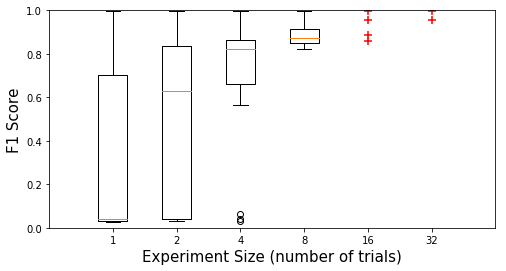
\includegraphics[width=0.8\linewidth]{images/random_hp_search_dnn_easy}
	\caption{Random hyperparameter search efficiency curves for the DNN using the simple dataset.}
	\label{fig:random_hp_search_dnn_easy}
\end{figure}

\begin{figure}[H]
	\centering
	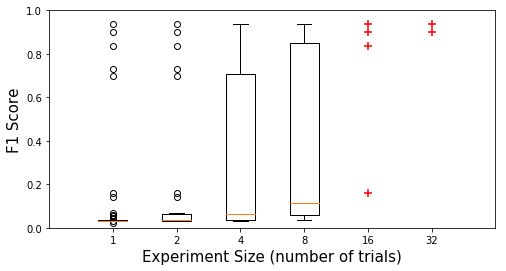
\includegraphics[width=0.8\linewidth]{images/random_hp_search_dnn_full}
	\caption{Random hyperparameter search efficiency curves for the DNN using the complete dataset.}
	\label{fig:random_hp_search_dnn_full}
\end{figure}


Figure \ref{fig:dense_hyperparameters_f1_score} shows the distribution of average validation dataset F1 score from the 5-folds cross validation for each hyperparameter. Conclusions based on these will suffer from a small sample size because few networks trained on the complete dataset achieved high validation dataset F1 scores. General trends in the simple dataset are more representative of actual hyperparameter performance compared to the complete dataset.

Sub-figure \ref{fig:dnn_learning_rate} shows that a learning rate less than 10$^{-2}$ should be used when conducting hyperparameter searches for spectroscopic datasets of similar complexity. This figure also shows that the complete dataset prefers a slower learning rate, with best performing networks using learning rates below 10$^{-3.5}$. Smaller learning rates should also be explored in future searches, if computationally feasible.

Sub-figure \ref{fig:dnn_dropout} shows that the dropout rate has a less obvious performance cutoff compared to the learning rate. This is likely because the dropout value does not have a large effect on training.

Sub-figure \ref{fig:dnn_batch_size} shows that the simple dataset works well in a variety of mini-batch sizes, while the complete dataset may require a larger mini-batch size.

Sub-figures \ref{fig:dnn_dense_nodes_total} and \ref{fig:dnn_dense_layers_total} show the effect of model capacity on performance. Model capacity is comparable to the number of free parameters of a model; too much capacity can lead to overfitting and too little capacity may be insufficient to fit complex data. Overfitting can be seen in the performance drop in three dense layers. Additional layers are unnecessary for problems of this difficulty with the hyperparameters explored. For the complete dataset a significant number of networks perform well with a total number of nodes between 250 and 1000. The simple dataset performed well with a wide range of total nodes.

Sub-figures \ref{fig:dnn_scaler} shows the effect of feature preprocessing on performance. L1 normalization performs very poorly due to the numerical scale of the features. Gradients computed with learning rates explored by the hyperparameter search are too small to significantly update the weights because the features are on the order 10$^{-3}$. Features explored by the other methods are typically between 10$^{0}$ - 10$^{2}$. Scaling spectra using the $sqrt$ of their features makes networks perform well for both datasets. In particular, using $sqrt-max$ scaling produces the most models with high validation dataset F1 scores.

\newcommand{\bluecircle}{\raisebox{2pt}{\tikz{\filldraw[color=blue!60, fill=blue!60, very thick] circle (1.5mm);}}}
\definecolor{darkgreen}{rgb}{0,0.3,0}

\begin{figure}[H]
     \centering
     \begin{subfigure}[b]{0.49\textwidth}
         \centering
         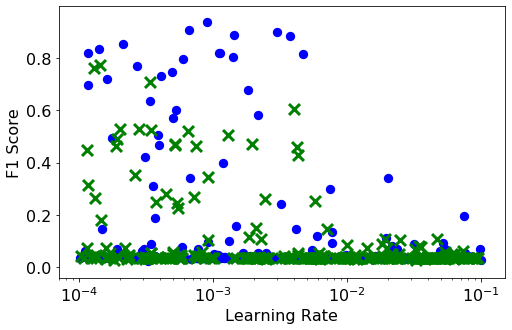
\includegraphics[width=\textwidth]{images/dnn_learning_rate.png}
         \caption{}
         \label{fig:dnn_learning_rate}
     \end{subfigure}
     \hfill
     \begin{subfigure}[b]{0.49\textwidth}
         \centering
         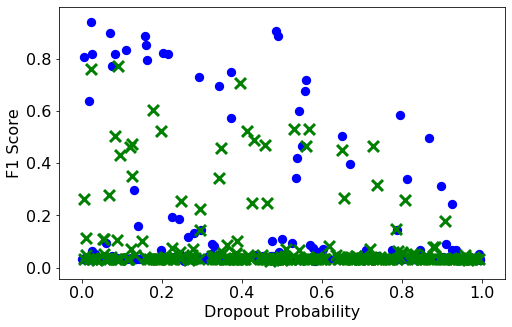
\includegraphics[width=\textwidth]{images/dnn_dropout.png}
         \caption{}
         \label{fig:dnn_dropout}
     \end{subfigure}

     \begin{subfigure}[b]{0.49\textwidth}
         \centering
         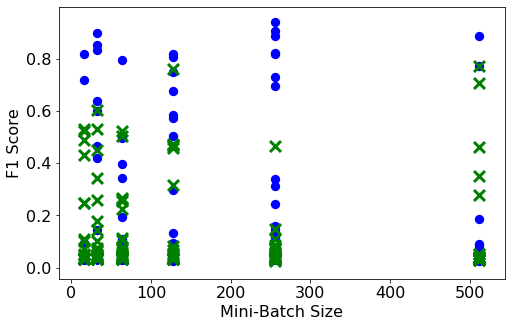
\includegraphics[width=\textwidth]{images/dnn_batch_size.png}
         \caption{}
         \label{fig:dnn_batch_size}
     \end{subfigure}
     \hfill
     \begin{subfigure}[b]{0.49\textwidth}
         \centering
         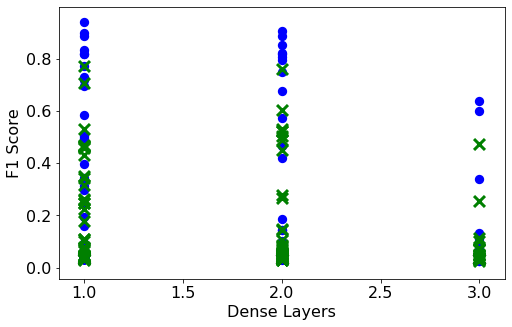
\includegraphics[width=\textwidth]{images/dnn_dense_layers_total.png}
         \caption{}
         \label{fig:dnn_dense_layers_total}
     \end{subfigure}

    \begin{subfigure}[b]{0.49\textwidth}
         \centering
         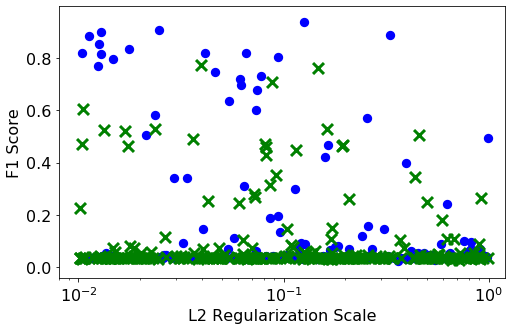
\includegraphics[width=\textwidth]{images/dnn_l2_reg.png}
         \caption{}
         \label{fig:dnn_l2_reg}
     \end{subfigure}
     \hfill
     \begin{subfigure}[b]{0.49\textwidth}
         \centering
         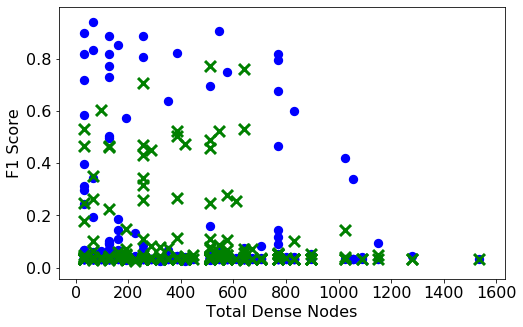
\includegraphics[width=\textwidth]{images/dnn_dense_nodes_total.png}
         \caption{}
         \label{fig:dnn_dense_nodes_total}
     \end{subfigure}     

    \begin{subfigure}[b]{0.49\textwidth}
        \centering
        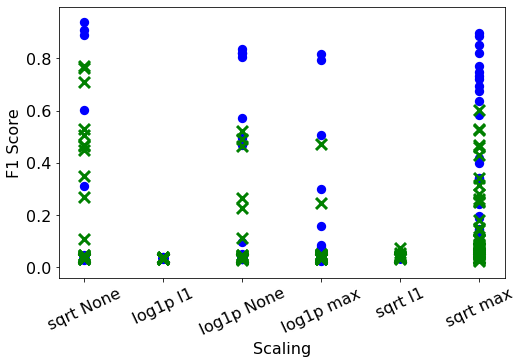
\includegraphics[width=\textwidth]{images/dnn_scaler.png}
         \caption{}
        \label{fig:dnn_scaler}
    \end{subfigure}
    \hfill
    \begin{subfigure}[b]{0.49\textwidth}
        \centering
        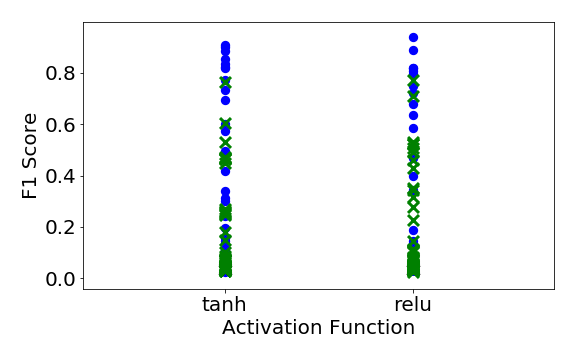
\includegraphics[width=\textwidth]{images/dnn_activation_function.png}
         \caption{}
        \label{fig:dnn_activation_function}
    \end{subfigure}
        \begin{tabular}{r@{ : }l r@{ : }l}
			\textcolor{darkgreen}{\textbf{\large{X}}} & Complete Dataset & \bluecircle & Simple Dataset \\
		\end{tabular}
        \caption{Effect of dense hyperparameters on the validation dataset's final F1 score.}
        \label{fig:dense_hyperparameters_f1_score}
\end{figure}


% \subsubsection{Hyperparameter Search Results - Autoencoders}

% Now that we know optimized autoencoder architectures for the DNN, we need to optimize training hyperparameters. 

% https://machinelearningmastery.com/activation-regularization-for-reducing-generalization-error-in-deep-learning-neural-networks/

% \cite{Ranzato2007} Fig 6 shows you can freeze the unsupervised feature extraction network and update the classifier if you have enough data.

% Sparse denoising autoencoders are included in in this work as feature extraction and dimension reduction techniques. Both autoencoders employ regularization techniques to ensure useful representations are learned. Both models includes $l1$ activity regularization as a method to induce sparsity on the networks activations, which increases generalization \cite{Goodfellow-et-al-2016}. 

% Show how well autoencoders worked at spectrum reconstruction and background subtraction. See if there's a large difference between doing background subtraction and 
\begin{table}[H]
\centering
\caption{Optimum DNN hyperparameter combination found for the simple and complete dataset.}
\label{table:hyperparameter_opt_parameters_DNN}
\begin{tabular}{lll}
\hline
\multirow{2}{*}{\textbf{Hyperparameter}} & \multicolumn{2}{l}{\textbf{Optimum Value}} \\
 & \textbf{Simple Dataset} & \textbf{Complete Dataset} \\ \hline
Dense Layer Hidden Nodes & 64 & 32 \\
Initial Learning Rate & 0.00089 & 0.00024 \\
L2 Regularization Strength & 0.13 & 0.0097 \\
Dropout Frequency & 0.023 & 0.16 \\
Batch Size & 256 & 16 \\
Activation Function & relu & relu \\
Input Scaling & sqrt & sqrt-max \\ 
Total Trainable Weights & 67550 & 540190 \\ \hline
\end{tabular}
\end{table}





\subsection{Convolution Architecture}

The architecture and training hyperparameters used to construct CNN's are shown in Table \ref{table:hyperparameter_dataset_parameters_CNN}. Note, as with the DNN the number of densely connected nodes decreased with each subsequent layer. A smaller range of batch sizes was searched in the CNN compared to the DNN due to computational constraints.

\begin{table}[H]
\centering
\caption{Range of hyperparameters explored for the CNN.}
\label{table:hyperparameter_dataset_parameters_CNN}
\begin{tabular}{lll}
\hline
\textbf{Hyperparameter} & \textbf{Hyperparameter Range} & \textbf{Sampling} \\ \hline
Filter Kernels in Each Layer& \begin{tabular}[l]{@{}l@{}} 4 \\ 8 \\ 16 \\ 32 \\ 4 - 8 \\ 8 - 16 \\ 16 - 32 \\ 4 - 8 - 16 \\  8 - 16 - 32 \end{tabular} & Uniform \\
Filter Kernel Lengths & 2, 4, 8, 16 & Uniform \\
Pooling size & 2, 4, 8, 16 & Uniform \\
Number of Dense Layers & 1 - 3 & Uniform \\
Nodes in Dense Layers & 10 - 1000 & Log-Uniform \\
Initial Learning Rate & 10$^{-4}$ - 10$^{-1}$ & Log-Uniform \\
L2 Regularization Strength & 10$^{-3}$ - 10$^{0}$ & Log-Uniform \\
Dropout Frequency & 0 - 1 & Uniform \\
Batch Size & 16, 32 & Uniform \\
Activation Function & tanh, relu & Uniform \\
Input Scaling & \begin{tabular}[l]{@{}l@{}}sqrt \\ sqrt-max \\ sqrt-L1 norm \\ log1p \\ log1p-max \\ log1p-L1 norm\end{tabular} & Uniform \\ \hline
\end{tabular}
\end{table}


Random efficiency experiment curves for the CNN trained on the simple and complete datasets are shown in Figures \ref{fig:random_hp_search_cnn_easy} and \ref{fig:random_hp_search_cnn_full}. Similar to the dense network, a large number of hyperparameter combinations did not reduce their validation dataset's F1 score in the training set in enough epochs and their training was ended early. Contrary to the DNN, the median validation dataset's F1 score in both datasets smoothly increased with additional trials. Both datasets achieved validation dataset F1 scores above 90$\%$. This demonstrates that the hyperparameter bounds used for both problems are well suited to the problems and that the CNN architectures explored in this search have more potential than the DNN architectures for gamma-ray spectroscopy. As with the DNN, validation dataset F1 scores on the simple dataset are higher than the validation dataset F1 scores on the complete dataset.

\begin{figure}[H]
	\centering
	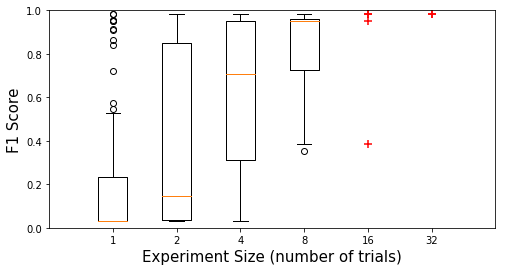
\includegraphics[width=0.8\linewidth]{images/random_hp_search_cnn_easy}
	\caption{Random hyperparameter search efficiency curves for the CNN using the simple dataset.}
	\label{fig:random_hp_search_cnn_easy}
\end{figure}

\begin{figure}[H]
	\centering
	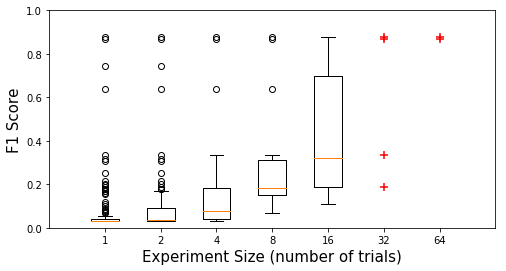
\includegraphics[width=0.8\linewidth]{images/random_hp_search_cnn_full}
	\caption{Random hyperparameter search efficiency curves for the CNN using the complete dataset.}
	\label{fig:random_hp_search_cnn_full}
\end{figure}


Figure \ref{fig:cnn_hyperparameters_f1_score} shows the distribution of hyperparameters searched for the CNN and their average validation dataset F1 scores from the 5-folds cross validation. Similar to the DNN, few networks trained on the complete dataset achieved high validation dataset F1 scores. Conclusions based on these diagrams suffer from small (albeit larger than the DNN) sample sizes.

The CNN's training performance is largely agnostic to many hyperparameters, including those associated with the dense part of the CNN. Figure \ref{fig:cnn_hyperparameters_f1_score} shows that both datasets train similarly over a wide range of learning rates below 10$^{-2}$, dense layer dropout rates below 0.8, L2 regularization scales below 10$^{-1}$, between 50 - 200 total dense nodes, and both mini-batch sizes.

The CNN's training performance on the complete dataset is sensitive to hyperparameters related to model capacity. The total number of convolutional layers have the largest affect on the performance of models trained using the complete dataset. Because of the additional complexity in the complete dataset, deeper networks - which extract more abstract features - are necessary for good performance. CNNs with additional convolutional layers should be explored for problems of similar complexity. Additional dense layers did not provide the same boost in performance. Models trained using the simple dataset perform well with a large range of total dense layers while the complete dataset performs well with fewer layers, achieving the best validation dataset F1 score with a two layers. Simple and complete models with three dense layers have maximum F1 scores lower than two or three dense layers.

Performance is also sensitive to other convolutional hyperparameters. Models trained using the simple datasets perform well with each convolutional pooling size. As a general trend, models trained with the complete dataset perform better with larger convolutional pooling sizes. Longer pooling sizes add more shift and scale invariance, which is more important in the complete dataset due to a wider range of detector gain settings. Longer pooling sizes are necessary to incorporate photopeaks and Compton continua, where smaller pooling sizes may be sufficient to retain only photopeak information. Identifying the photopeaks may be enough to identify isotopes in the simple dataset because there are fewer confounding variables. Convolutional kernel lengths of 16 are required for optimal performance for both datasets. The preference for depth in the convolutional part of the CNN is also seen in the number of convolutional filters.

The effect of scaling on performance was similar to the DNN. Using $sqrt$ scaling yielded the best performing networks, especially when tied with $max$ normalization.


\begin{figure}[H]
     \centering
     \begin{subfigure}[b]{0.49\textwidth}
         \centering
         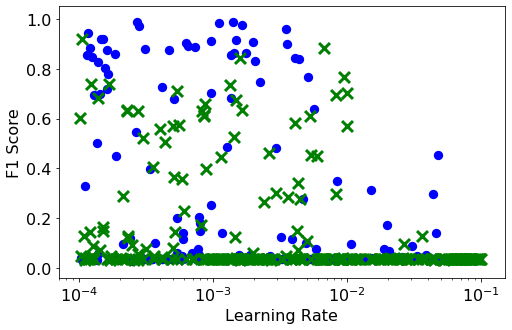
\includegraphics[width=\textwidth]{images/cnn_learning_rate.png}
         \caption{}
         \label{fig:cnn_learning_rate}
     \end{subfigure}
     \hfill
     \begin{subfigure}[b]{0.49\textwidth}
         \centering
         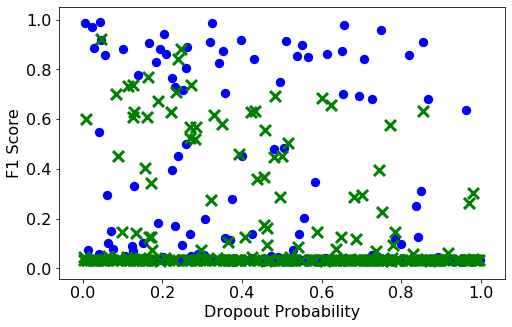
\includegraphics[width=\textwidth]{images/cnn_dropout.png}
         \caption{}
         \label{fig:cnn_dropout}
     \end{subfigure}

     \begin{subfigure}[b]{0.49\textwidth}
         \centering
         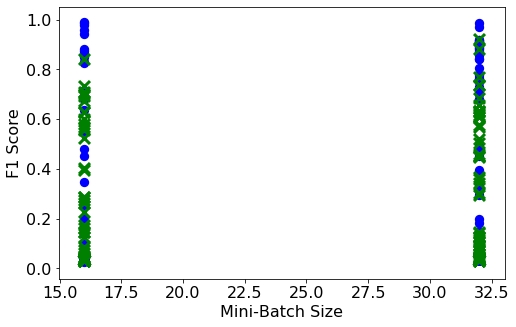
\includegraphics[width=\textwidth]{images/cnn_batch_size.png}
         \caption{}
         \label{fig:cnn_batch_size}
     \end{subfigure}
     \hfill
     \begin{subfigure}[b]{0.49\textwidth}
         \centering
         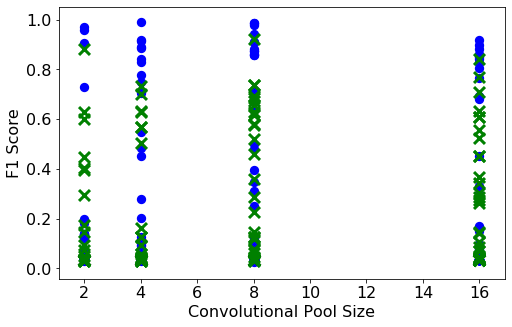
\includegraphics[width=\textwidth]{images/cnn_pooling_size.png}
         \caption{}
         \label{fig:cnn_pooling_size}
     \end{subfigure}

    \begin{subfigure}[b]{0.49\textwidth}
         \centering
         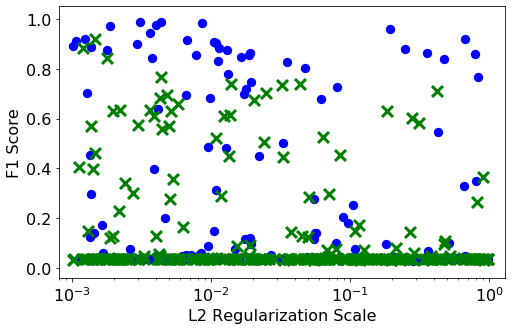
\includegraphics[width=\textwidth]{images/cnn_l2_reg.png}
         \caption{}
         \label{fig:cnn_l2_reg}
     \end{subfigure}
     \hfill
     \begin{subfigure}[b]{0.49\textwidth}
         \centering
         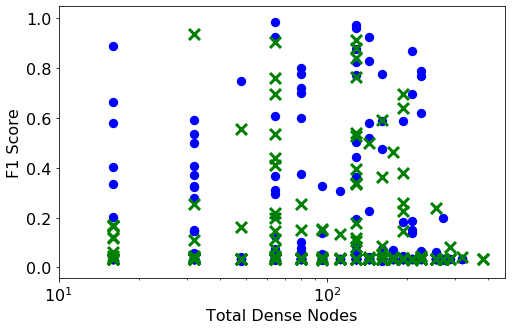
\includegraphics[width=\textwidth]{images/cnn_dense_nodes_total.png}
         \caption{}
         \label{fig:cnn_dense_nodes_total}
     \end{subfigure}  
     
     \begin{subfigure}[b]{0.49\textwidth}
         \centering
         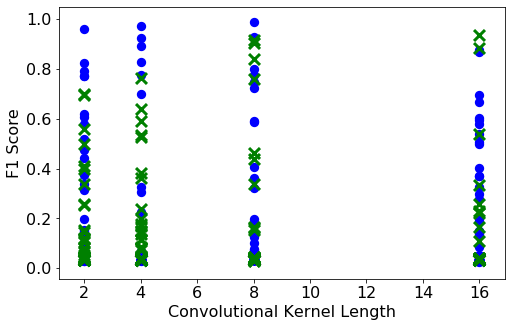
\includegraphics[width=\textwidth]{images/cnn_kernel_length.png}
         \caption{}
         \label{fig:cnn_kernel_length}
     \end{subfigure}
     \hfill
     \begin{subfigure}[b]{0.49\textwidth}
         \centering
         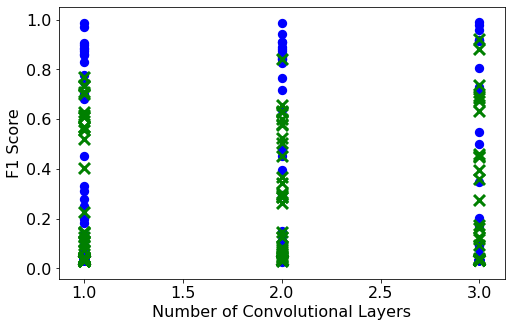
\includegraphics[width=\textwidth]{images/cnn_num_conv_layers.png}
         \caption{}
         \label{fig:cnn_num_conv_layers}
     \end{subfigure}  
	\begin{tabular}{r@{ : }l r@{ : }l}
		\textcolor{darkgreen}{\textbf{\large{X}}} & Complete Dataset & \bluecircle & Simple Dataset \\
	\end{tabular}
    \caption{Effect of CNN hyperparameters on the validation dataset's final F1 score.}
\end{figure}

\begin{figure} \ContinuedFloat
    \centering
    
    \begin{subfigure}[t]{0.49\textwidth}
        \centering
        % \raisebox{-0.49cm}{
        \includegraphics[width=\textwidth]{images/cnn_scaler.png}
        % }
        \caption{}
        \label{fig:cnn_scaler}
    \end{subfigure}
    \hfill
    \begin{subfigure}[t]{0.49\textwidth}
        \centering
        \includegraphics[width=\textwidth]{images/cnn_filter_structure.png}
        \caption{}
        \label{fig:cnn_filter_structure}
    \end{subfigure}
    
    \begin{subfigure}[t]{0.49\textwidth}
        \centering
        \includegraphics[width=\textwidth]{images/cnn_dense_layers_total.png}
        \caption{}
        \label{fig:cnn_dense_layers_total}
    \end{subfigure}
	\hfill
	\begin{subfigure}[t]{0.49\textwidth}
		\centering
		\includegraphics[width=\textwidth]{images/cnn_activation_function.png}
		\caption{}
		\label{fig:cnn_activation_function}
	\end{subfigure}

		\begin{tabular}{r@{ : }l r@{ : }l}
			\textcolor{darkgreen}{\textbf{\large{X}}} & Complete Dataset & \bluecircle & Simple Dataset \\
		\end{tabular}
        \caption{Effect of CNN hyperparameters on the validation dataset's final F1 score.}
        \label{fig:cnn_hyperparameters_f1_score}
\end{figure}

\begin{table}[H]
\centering
\caption{Optimum CNN hyperparameter combination found for the simple and complete dataset.}
\label{table:hyperparameter_opt_parameters_CNN}
\begin{tabular}{lll}
\hline
\multirow{2}{*}{\textbf{Hyperparameter}} & \multicolumn{2}{l}{\textbf{Optimum Value}} \\
 & \textbf{Simple Dataset} & \textbf{Complete Dataset} \\ \hline
Filter Kernels in Each Layer & 4 - 8 - 16 & 8 - 16 - 32 \\
Filter Kernel Length & 16 & 16 \\
Pooling size & 4 & 8 \\
Dense Layer Structure & 128 - 64 & 128 - 64 \\
Initial Learning Rate & 0.0014 & 0.00010 \\
L2 Regularization Strength & 0.0044 & 0.0015 \\
Dropout Frequency & 0.042 & 0.045 \\
Batch Size & 16 & 32 \\
Activation Function & tanh & tanh \\
Input Scaling & sqrt-max & sqrt-max \\ \hline
\end{tabular}
\end{table}

% \begin{table}[H]
% \centering
% \caption{Range of hyperparameters explored for the CNN.}
% \label{table:hyperparameter_dataset_parameters_CNN}
% \begin{tabular}{ccc}
% % \cline{2-3}
%  & Hyperparameter Range & Sampling \\ \hline
% \multicolumn{1}{c}{} & \begin{tabular}[c]{@{}c@{}}(4)   (8)   (16)    (32)\\ (4, 8)  (8, 16)  (16, 32)\\ (4, 8, 16)   (8, 16, 32)\end{tabular} & Uniform \\
% \multicolumn{1}{c}{} & 2, 4, 8, 16 & Uniform \\
% \multicolumn{1}{c}{} & 2, 4, 8, 16 & Uniform \\
% \multicolumn{1}{c}{} & 1 - 3 & Uniform \\
% \multicolumn{1}{c}{} & 10 - 1000 & Log-Uniform \\
% \multicolumn{1}{c}{} & 10$^{-4}$ - 10$^{-1}$ & Log-Uniform \\
% \multicolumn{1}{c}{} & 10$^{-3}$ - 10$^{0}$ & Log-Uniform \\
% \multicolumn{1}{c}{Dropout Frequency} & 0 - 1 & Uniform \\
% \multicolumn{1}{c}{Batch Size} & 2$^{4}$ - 2$^{6}$ & Power of Two \\
% \multicolumn{1}{c}{Activation Function} & tanh, relu & Uniform \\
% \multicolumn{1}{c}{Input Scaling} & \begin{tabular}[c]{@{}c@{}}sqrt, sqrt-max,\\sqrt-L1 Norm,\\ log1p-None, log1p-max,\\ log1p-L1 Norm\end{tabular} & Uniform \\
% \end{tabular}
% \end{table}

\subsection{Autoencoder Architectures} \label{section_autoencoder_archetectures}

Without an autoencoder, a single ANN has to learn multiple tasks to identify isotopes. An ANN would have to simultaneously identify the detector calibration, background signal, and source signal. By pretraining each network using an autoencoder to reconstruct a background-subtracted spectrum, the task of isotope identification is simplified for the ANN. To determine if using pretrained models results in more accurate identifications, a DAE and CAE were trained using the model parameters found in the hyperparameter search.

% (Tables \ref{table:hyperparameter_dataset_easy_parameters} and \ref{table:hyperparameter_dataset_full_parameters})
Pretraining was performed using a dataset of 10000 samples generated using the simple and complete dataset parameters. Because of the implicit regularization of the undercomplete encoding and the denoising background subtracting process, neither network uses additional regularization when training. The initial learning rate of each autoencoder was set to 10$^{-5}$.

% This section will explain the hyperparameter structures searched. The autoencoder used is a undercomplete denoising autoencoder \cite{Goodfellow-et-al-2016}. Because the denoising operation performs regularization implicitly, no additional regularization is added to the autoencoders. 

% The autoencoder structures are found using a grid search. The autoencoders that reproduce the background subtracted signal the best are used in a dense random hyperparameter search as the signal preprocessing.


% The DAE structure is based on the dense hyperparameter search. The DAE trained on both datasets uses the same parameters as Table \ref{table:hyperparameter_dataset_parameters_DNN} without regularization and with an initial learning rate set to 10$^{-5}$. The DAE does not use L2 regularization or dropout due to the implicit regularization of the undercomplete encoding and the denoising background subtracting process.

% \begin{table}[H]
% \centering
% \caption{Optimum DNN hyperparameter combination found for the simple and complete dataset.}
% \label{table:hyperparameter_dataset_parameters_DNN}
% \begin{tabular}{ccc}
% \multirow{2}{*}{Hyperparameter} & \multicolumn{2}{c}{Optimum Value} \\
%  & Simple Dataset & Complete Dataset \\ \hline
% Dense Layer Structure & (64) & (32) \\
% Initial Learning Rate & 10$^{-5}$ & 10$^{-5}$ \\
% Batch Size & 256 & 16 \\
% Activation Function & relu & relu \\
% Input Scaling & sqrt & sqrt-max
% \end{tabular}
% \end{table}

% The CAE structure is based on the convolutional hyperparameter search. The CAE's trained on both datasets use the same parameters as Table \ref{table:hyperparameter_dataset_parameters_CNN} without regularization and with an initial learning rate set to 10$^{-5}$.


% \section{Summary of Final Model Architectures}


% This section discusses performance differences between the DNN, CNN, CAE-DNN, and DAE-DNN. These differences will be based on the final testing set error for all models.  






% Removing this for now

\chapter{Urban Source Identification Results and Discussion}

% Compare how well we identify shielded/unshielded isotopes when training set has shielding, doesn't have shielding. 

% Compare how well we identify isotopes over different distances if training set has one vs many distances

% Compare how well we identify isotopes with different calibration sampling granularity 

% https://e-reports-ext.llnl.gov/pdf/312592.pdf holy shit they show common false positive isotopes and we see a lot of overlap



\section{Problem Description and Training Dataset Overview}

This chapter applies machine learning algorithms to solve the problem of a identifying a radioactive source in an urban environment where a source may be present. This scenario is applicable when performing source interdiction searching cargo containers, vehicles at boarder crossings, or security at high profile events. Urban environments present unique challenges to gamma-ray spectroscopy. Background radiation can change over city blocks due to different concentrations of uranium and thorium in building materials. Sources may be purposely shielded by unknown amounts of material to obscure their gamma-ray signal.





\section{Online Data Augmentation Method}

Because simulating a dataset with sufficient combinations of available data augmentation - seen in Tables \ref{table:all_fixed_simulation_parameters} and \ref{table:all_variable_simulation_parameters} - online data augmentation techniques are employed. Online data augmentation has the benefit of implicitly regularizing the models.

Steps in the data augmentation process are:
\begin{enumerate}
  \item Randomly choose a background template with the same FWHM as the source template
  \item Rebin source and background template with a random calibration
  \item Apply the LLD to both templates
  \item Normalize both templates by the sum of their respective counts 
  \item Scale both signals by their respective total counts
  \begin{itemize}
     \item Counts defined by randomly chosen background counts per second, integration time, and signal to background ratio
   \end{itemize}
  \item Add both signals 
  \item Poisson sample the resulting signal
\end{enumerate}


\section{Learning Curve Comparison for Fixed-size Datasets and Online Data Augmentation Datasets}

In this section we use learning curves to quantify how well the online data augmentation improved testing error. Learning curves are [definition, explanation]. Learning curves are used to determine a few things. We will use them to do [the following].

First, They are used as a sanity check, to make sure we are sampling our input space with enough granularity. To know we are sampling well enough, we should be sampling in a region where the curves are flat for both algorithms.

Secondly, Learning curves give us insight into which algorithm works better on the hyperparameter optimization dataset and simple version of the problem. We're expecting the CNN to outperform the DNN due to theoretical benefits of convolution architectures for our problem. We can also compare this curve to the final learning curves for the final datasets.


\begin{figure}[H]
	\centering
	\includegraphics[width=0.8\linewidth]{model_choice_hyperparameter_search_images/learning_curve_dummy}
	\caption{Learning curves from the best DNN with best performance from online data augmentation. Shown: learning curve example.}
	\label{fig:learning_curves}
\end{figure}



\begin{figure}[H]
	\centering
	\includegraphics[width=0.8\linewidth]{model_choice_hyperparameter_search_images/learning_curve_dummy}
	\caption{Learning curves from the best CNN with best performance from online data augmentation. Shown: learning curve example.}
	\label{fig:learning_curves}
\end{figure}


\section{Generalization Performance Evaluation}

In this section we analyze the generalization performance of each network on various datasets. To quantify performance on a range of spectra qualities, the F1-scores are shown over integration time and for different signal to background ratios. When the error between models differs significantly or is particularly large, confusion matrices are included to show what isotopes are problematic.

Could also change the underlying distribution away from the training set by simulating a new template dataset with a different clutter parameter.

A default dataset will be modified. The default dataset will be  correspond to unshielded templates. 

\subsection{Generalization Performance on Source-Detector Distance and Height Off Ground}

In this section we analyze the generalization performance of each network on changes in source-detector distance and height. This tests if each model is sensitive to changes in the Compton continuum due to environmental scattering. Good performance in these simulated data may indicate better performance in real data.

To test generalization performance, datasets are simulated with unshieled spectral templates with a FWHM of 7.5. 


\begin{figure}[H]
     \centering
     \begin{subfigure}[b]{0.9\textwidth}
         \centering
         \includegraphics[width=\textwidth]{images/results_easy_distance_comparison}
         \caption{Simple Dataset.}
         \label{fig:results_easy_distance_comparison_simple}
     \end{subfigure}

     \begin{subfigure}[b]{0.9\textwidth}
         \centering
         \includegraphics[width=\textwidth]{images/results_easy_distance_comparison}
         \caption{Full Dataset.}
         \label{fig:results_easy_distance_comparison_full}
     \end{subfigure}
        \caption{F1 score for all models trained on the simple dataset. Datasets included here used various source-detector distance.}
        \label{fig:results_easy_distance_comparison}
\end{figure}

\begin{figure}[H]
     \centering
     \begin{subfigure}[b]{0.9\textwidth}
         \centering
         \includegraphics[width=\textwidth]{images/results_easy_distance_comparison}
         \caption{Simple Dataset.}
         \label{fig:results_easy_distance_comparison_simple}
     \end{subfigure}

     \begin{subfigure}[b]{0.9\textwidth}
         \centering
         \includegraphics[width=\textwidth]{images/results_easy_distance_comparison}
         \caption{Full Dataset.}
         \label{fig:results_easy_distance_comparison_full}
     \end{subfigure}
        \caption{F1 score for all models trained on the simple dataset. Datasets included here used various source-detector heights.}
        \label{fig:results_easy_distance_comparison}
\end{figure}



\subsection{Generalization Dependence on Full-Width-at-Half-Max}

Datasets were constructed with various Gaussian energy broadening function. This is to 

\begin{figure}[H]
     \centering
     \begin{subfigure}[b]{0.9\textwidth}
         \centering
         \includegraphics[width=\textwidth]{images/results_easy_distance_comparison}
         \caption{Simple Dataset.}
         \label{fig:results_easy_distance_comparison_simple}
     \end{subfigure}

     \begin{subfigure}[b]{0.9\textwidth}
         \centering
         \includegraphics[width=\textwidth]{images/results_easy_distance_comparison}
         \caption{Full Dataset.}
         \label{fig:results_easy_distance_comparison_full}
     \end{subfigure}
        \caption{F1 score for all models trained on the simple dataset. Datasets included here used various Gaussian energy broadening functions.}
        \label{fig:results_easy_distance_comparison}
\end{figure}


\subsection{Generalization Dependence on Shielding.}

Datasets were simulated with and without shielding. 

\begin{figure}[H]
     \centering
     \begin{subfigure}[b]{0.9\textwidth}
         \centering
         \includegraphics[width=\textwidth]{images/results_easy_distance_comparison}
         \caption{Simple Dataset.}
         \label{fig:results_easy_distance_comparison_simple}
     \end{subfigure}

     \begin{subfigure}[b]{0.9\textwidth}
         \centering
         \includegraphics[width=\textwidth]{images/results_easy_distance_comparison}
         \caption{Full Dataset.}
         \label{fig:results_easy_distance_comparison_full}
     \end{subfigure}
        \caption{F1 score for all models trained on the simple dataset. Datasets included here used various amounts of shielding.}
        \label{fig:results_easy_distance_comparison}
\end{figure}


\begin{figure}[H]
     \centering
     \begin{subfigure}[b]{0.8\textwidth}
         \centering
         \includegraphics[width=\textwidth]{model_choice_hyperparameter_search_images/conf_matrix_example.png}
         \caption{Simple Training Dataset.}
         \label{fig:results_easy_distance_comparison_simple}
     \end{subfigure}

     \begin{subfigure}[b]{0.8\textwidth}
         \centering
         \includegraphics[width=\textwidth]{model_choice_hyperparameter_search_images/conf_matrix_example.png}
         \caption{Full Training Dataset.}
         \label{fig:results_easy_distance_comparison_full}
     \end{subfigure}
        \caption{Confusion matrices for the dataset with 60\% shielding.}
        \label{fig:results_easy_distance_comparison}
\end{figure}

\begin{figure}[H]
     \centering
     \begin{subfigure}[b]{0.49\textwidth}
         \centering
         \includegraphics[width=\textwidth]{model_choice_hyperparameter_search_images/conf_matrix_example.png}
         \caption{Simple Training Dataset.}
         \label{fig:results_easy_distance_comparison_simple}
     \end{subfigure}
     \hfill
     \begin{subfigure}[b]{0.49\textwidth}
         \centering
         \includegraphics[width=\textwidth]{model_choice_hyperparameter_search_images/conf_matrix_example.png}
         \caption{Full Training Dataset.}
         \label{fig:results_easy_distance_comparison_full}
     \end{subfigure}
     
     \begin{subfigure}[b]{0.49\textwidth}
         \centering
         \includegraphics[width=\textwidth]{model_choice_hyperparameter_search_images/conf_matrix_example.png}
         \caption{Simple Training Dataset.}
         \label{fig:results_easy_distance_comparison_simple}
     \end{subfigure}
     \hfill
     \begin{subfigure}[b]{0.49\textwidth}
         \centering
         \includegraphics[width=\textwidth]{model_choice_hyperparameter_search_images/conf_matrix_example.png}
         \caption{Full Training Dataset.}
         \label{fig:results_easy_distance_comparison_full}
     \end{subfigure}
     
        \caption{Confusion matrices for the dataset with 60\% shielding.}
        \label{fig:results_easy_distance_comparison}
\end{figure}



\subsection{Generalization Dependence on Calibration.}

Datasets were simulated with various gain and offset setting.

\begin{figure}[H]
     \centering
     \begin{subfigure}[b]{0.9\textwidth}
         \centering
         \includegraphics[width=\textwidth]{images/results_easy_distance_comparison}
         \caption{Simple Dataset.}
         \label{fig:results_easy_distance_comparison_simple}
     \end{subfigure}

     \begin{subfigure}[b]{0.9\textwidth}
         \centering
         \includegraphics[width=\textwidth]{images/results_easy_distance_comparison}
         \caption{Full Dataset.}
         \label{fig:results_easy_distance_comparison_full}
     \end{subfigure}
        \caption{F1 score for all models trained on the simple dataset. Datasets included here used various gain and offset settings.}
        \label{fig:results_easy_distance_comparison}
\end{figure}



\subsection{Generalization Dependence on Changing Background.}

Datasets were simulated with backgrounds different from the training set and real measured background. It is expected that the full dataset will mistake background for isotopes more often than the simple dataset because photopeaks are decreased by shielding.


\begin{figure}[H]
     \centering
     \begin{subfigure}[b]{0.9\textwidth}
         \centering
         \includegraphics[width=\textwidth]{images/results_easy_distance_comparison}
         \caption{Simple Dataset.}
         \label{fig:fig:results_easy_background_simulated_simple}
     \end{subfigure}

     \begin{subfigure}[b]{0.9\textwidth}
         \centering
         \includegraphics[width=\textwidth]{images/results_easy_distance_comparison}
         \caption{Full Dataset.}
         \label{fig:fig:results_easy_background_simulated_full}
     \end{subfigure}
        \caption{F1 score for all models trained on the simple dataset. Datasets included here used various amounts of shielding.}
        \label{fig:results_easy_background_simulated}
\end{figure}



Figure \ref{fig:results_full_background_inject} shows the identification performance on 

\begin{figure}[H]
     \centering
     \begin{subfigure}[b]{0.9\textwidth}
         \centering
         \includegraphics[width=\textwidth]{images/results_easy_distance_comparison}
         \caption{Simple Dataset.}
         \label{fig:results_full_background_inject_simple}
     \end{subfigure}

     \begin{subfigure}[b]{0.9\textwidth}
         \centering
         \includegraphics[width=\textwidth]{images/results_easy_distance_comparison}
         \caption{Full Dataset.}
         \label{fig:results_full_background_inject_full}
     \end{subfigure}
        \caption{F1 score for all models trained on the full dataset. Datasets included here used various amounts of shielding.}
        \label{fig:results_full_background_inject}
\end{figure}


% \section{Results from training all models}

% When training final models, two main questions need to be addressed: how good is a given architecture at solving a problem on its training dataset and how good is a given dataset at generalizing to outside examples.

% To determine how good a given architecture solves a problem, asymptotic convergence of the models performance needs to be measured. Because of the inherent stochastic nature of training machine learning algorithms (different random weight initialization, different mini-batches chosen during training, different data augmentation manifestations), each time a new network is trained the networks parameters and results will differ. This means a single trained instance of some model A may outperform a single trained instance of model B by chance, despite model B being an overall superior architecture. To more realistically compare how models perform on some dataset, a number of networks can be trained and their average performance compared. This is a method called bagging.

% \subsection{Asymptotic Model Performance on Training Dataset}

% For the best DNN and CNN architectures found in the hyperparameter search, using 'enough' data data samples as found in the hyperparameter search, 30 networks are trained. Their performance is observed in Figure \ref{fig:asymptotic_performance}.


%% Can also include performance using templates with extreme augmentation
% \begin{figure}[H]
% 	\centering
% 	\includegraphics[width=0.8\linewidth]{model_choice_hyperparameter_search_images/asymptotic_performance_dummy}
% 	\caption{Asymptotic model performance for both the CNN and DNN on the training sets.}
% 	\label{fig:asymptotic_performance}
% \end{figure}

% Using N models as representative of asymptotic performance, justified in Figure \ref{fig:asymptotic_performance}, we can check out the confusion matrix associated with the test dataset to gain insight into how the algorithm is performing poorly and predict future shortcomings.


%% Can also include performance using templates with extreme augmentation
% \begin{figure}[H]
% 	\centering
% 	\includegraphics[width=0.8\linewidth]{model_choice_hyperparameter_search_images/conf_matrix_example}
% 	\caption{Asymptotic model performance for both the CNN and DNN on the training sets.}
% 	\label{fig:asymptotic_performance}
% \end{figure}

% Can also analyze how changing a threshold would affect precision/recall!

% \subsection{Results from training models using extreme data augmentation vs Data Augmentation grid sampling}

% Show learning curve between models 
% Instead of training examples on x-axis, plot against "number of divisions" (which also has a number of training examples included...)
% Note! You can start holding parameters constant to see what parameter the model is having difficulty explaining
% \begin{figure}[H]
%	\centering
%	\includegraphics[width=0.8\linewidth]{model_choice_hyperparameter_search_images/learning_curve_dummy}
%	\caption{Learning curve example.}
%	\label{fig:Node}
%\end{figure}

%% Plot of average F1-score vs epochs for all models. Datasets include different detector model (use this as validation set) and same detector model with certain augmentation parameters frozen (or just the training set).


%% Plot of average F1-score vs epochs for all models. Datasets include different detector model (us this as validation set) and same detector model with certain augmentation parameters frozen (or just the training set).

\subsection{Results on Spectra for ANSI compliance}

This section shows model asymptotic performance vs integration time for ANSI compliance. Using N models (justified previously as asymptotic). 



\begin{table}[H]
\centering
\caption{Isotope combinations required for the ANSI standard \cite{ANSI}.}
\begin{tabular}{c}
\hline
$^{137}$Cs + depleted uranium (DU) \\ \hline
$^{99m}$Tc + HEU \\ \hline
$^{201}$Tl + HEU \\ \hline
$^{67}$Ga + HEU \\ \hline
$^{131}$I + WGPu \\ \hline
NORM + HEU \\ \hline
NORM + WGPu \\ \hline
\end{tabular}
\end{table}



\begin{figure}[H]
     \centering
     \begin{subfigure}[b]{0.9\textwidth}
         \centering
         \includegraphics[width=\textwidth]{images/results_easy_distance_comparison}
         \caption{Simple Dataset.}
         \label{fig:results_full_background_inject_simple}
     \end{subfigure}

     \begin{subfigure}[b]{0.9\textwidth}
         \centering
         \includegraphics[width=\textwidth]{images/results_easy_distance_comparison}
         \caption{Full Dataset.}
         \label{fig:results_full_background_inject_full}
     \end{subfigure}

        \caption{F1 score for models tested on ANSI isotope combinations.}
        \label{fig:results_full_background_inject}
\end{figure}



\subsection{Results on Measured Spectra}

This section shows model asymptotic performance vs integration time for a few different settings (different voltages, shielding)

To investigate how each model identified real spectra behind shielding and spectra with different calibrations, real spectra were measured. Sources include $^{137}$Cs, $^{60}$Co, $^{133}$Ba, and $^{152}$Eu. 


\subsubsection{Asymptotic Model Performance on Changing Voltage}

To see the generalization performance of the model to changing calibration, spectra with different voltages are recorded and their asymptotic performance compared.

Spectra were measured with different detector calibrations. A 2x2 Ortec NaI detector was set to 770 V, setting it's 1024th channel to 3 MeV. To capture a large range of calibrations, voltages varied from 720 V to 820 V in steps of 15 V. The $^{137}$Cs, $^{60}$Co, and $^{133}$Ba source had an activity of 1$\mu$C. For these sources, a source-to-detector distance of 14.25 mm was used to keep the cps on the detector from the source equal to the cps on the detector from background.

Figures \ref{fig:model_asymptotic_performance_co60} and \ref{fig:model_asymptotic_performance_cs137} show performance for isotopes with comparatively simple spectra.


\begin{figure}[H]
     \centering
     \begin{subfigure}[b]{0.9\textwidth}
         \centering
         \includegraphics[width=\textwidth]{images/results_easy_distance_comparison}
         \caption{$^{60}$Co}
         \label{fig:model_asymptotic_performance_co60}
     \end{subfigure}

     \begin{subfigure}[b]{0.9\textwidth}
         \centering
         \includegraphics[width=\textwidth]{images/results_easy_distance_comparison}
         \caption{$^{137}$Cs.}
         \label{fig:results_easy_distance_comparison_full}
     \end{subfigure}
     
     \begin{subfigure}[b]{0.9\textwidth}
         \centering
         \includegraphics[width=\textwidth]{images/results_easy_distance_comparison}
         \caption{$^{152}$Eu.}
         \label{fig:results_easy_distance_comparison_full}
     \end{subfigure}
     
     \begin{subfigure}[b]{0.9\textwidth}
         \centering
         \includegraphics[width=\textwidth]{images/results_easy_distance_comparison}
         \caption{$^{133}$Ba.}
         \label{fig:results_easy_distance_comparison_full}
     \end{subfigure}

        \caption{F1 score for all models trained on the simple dataset. Spectra measured with different gain settings.}
        \label{fig:results_easy_distance_comparison}
\end{figure}


\begin{figure}[H]
     \centering
     \begin{subfigure}[b]{0.9\textwidth}
         \centering
         \includegraphics[width=\textwidth]{images/results_easy_distance_comparison}
         \caption{$^{60}$Co}
         \label{fig:model_asymptotic_performance_co60}
     \end{subfigure}

     \begin{subfigure}[b]{0.9\textwidth}
         \centering
         \includegraphics[width=\textwidth]{images/results_easy_distance_comparison}
         \caption{$^{137}$Cs.}
         \label{fig:results_easy_distance_comparison_full}
     \end{subfigure}
     
     \begin{subfigure}[b]{0.9\textwidth}
         \centering
         \includegraphics[width=\textwidth]{images/results_easy_distance_comparison}
         \caption{$^{152}$Eu.}
         \label{fig:results_easy_distance_comparison_full}
     \end{subfigure}
     
     \begin{subfigure}[b]{0.9\textwidth}
         \centering
         \includegraphics[width=\textwidth]{images/results_easy_distance_comparison}
         \caption{$^{133}$Ba.}
         \label{fig:results_easy_distance_comparison_full}
     \end{subfigure}

        \caption{F1 score for all models trained on the full dataset. Spectra measured with different gain settings.}
        \label{fig:results_easy_distance_comparison}
\end{figure}





\chapter[Uranium Enrichment Regression \newline Results and Discussion]{Uranium Enrichment Regression Results and Discussion}

% great examples of various enriched U with a large range of detector resolutions https://www.lanl.gov/orgs/n/n1/docs/la_14206.pdf

Measuring uranium enrichment is difficult for a number of reasons. First, characteristic $^{235}$U gamma-rays are easily shielded. Second, restriction may be placed on inspectors performing measurements for treaty verification. Inspectors can face two major restrictions: a limited amount of time to measure data and the requirement for an information barrier. An information barrier is anything that restricts the inspector from measuring information outside of their specific target. For example, if an inspector measured the gamma-ray spectrum of an object using a high-resolution HPGe detector, they could extract information about the process used to process used to bred and enrich the material. This information could be a state secret, and thus would need to be protected with some barrier. The low-resolution inherent to NaI(Tl) is an information barrier for treaty verification measurements. An addition information barrier is an ANN which is trained to only extract enrichment information. 

This chapter demonstrates a validation demonstration applying \verb|annsa| to automated uranium enrichment measurements using NaI(Tl). In this chapter we discuss how we used MCNP and GADRAS-DRF to create spectral templates for training dataset simulation with \verb|annsa|. We also train and benchmark ANNs on simulated and measured enriched uranium spectra measured at the Nevada National Security Site and as part of a IAEA training exercise.


\section{Uranium Enrichment Measurement Background}

Verifying the enrichment of HEU through passive nondestructive analysis is important for nuclear safeguard applications and homeland security tasks. Passive nondestructive analysis, such as gamma-ray spectroscopy, is preferred to more accurate destructive methods due to its ability to operate quickly, preserve forensic evidence, and allow for remote measurements. The enriched uranium gamma-ray signatures visible in low-resolution detectors come from the decay of $^{238}$U, $^{235}$U, $^{232}$U, and the daughters of these isotopes. Figure \ref{fig:enriched_u_peaks_displayed} shows an example of a 27\% enriched uranium spectrum that displays $^{238}$U and $^{235}$U photopeaks. In low-resolution detectors, The primary photopeaks from $^{235}$U are at 144 keV, 163 keV, and 186 keV. The $^{238}$U daughter $^{234m}$Pa produces two main photopeaks at 766 keV and 1001 keV. $^{232}$U, only present in reprocessed uranium, produces a photopeak at 2.6 MeV from its $^{208}$Tl daughter.

\begin{figure}[H]
	\centering
	\includegraphics[width=0.8\linewidth]{images/enriched_u_peaks_displayed}
	\caption{27\% enriched uranium spectrum measured with a NaI(Tl) detector.}.
	\label{fig:enriched_u_peaks_displayed}
\end{figure}

Traditionally, the enrichment meter method is used to measure uranium enrichment in NaI(Tl) spectra \cite{Reilly1970}. This, and all enrichment measurement methods based on gamma-ray spectroscopy, only measures the enrichment of an object's surface to a depth of 0.26 cm and 0.74 cm for uranium metal and U$_{3}$O$_{8}$ powder, respectively \cite{Pandas}. At these material depths, the attenuation properties of uranium removes 99.8\% of the 186 keV signal. The enrichment meter method method exploits the proportionality between the activity of the 186 keV photon and the enrichment of $^{235}$U. The enrichment meter method works by finding calibration constants that relate counts in two ROIs,
%
\begin{align} \label{eq:enrichment_meter_principle}
E &= A  C_{ROI1} + B C_{ROI2} \\
\text{where } C_{ROI1} &= \text{counts in ROI1 [\# counts]} \nonumber \\
C_{ROI2} &= \text{counts in ROI2 [\# counts]} \nonumber \\
A &= \text{calibration constant} \nonumber \\
B &= \text{calibration constant,} \nonumber
\end{align}
%
to the measured material's enrichment. These ROIs are placed around the 186 keV peak and in the background region to the right of the peak. Finding these constants requires measuring two different uranium enrichment standards in the same configuration (shielding, scattering environment, source-detector distance). Once these calibration constants are measured, they can only be used in the same configuration as the reference standards. It is possible to extend this method to other shielding configurations, but this introduces a risk of adding systematic errors. An automated version of this method called NaIGEM (NaI(Tl) Gamma Enrichment Measurements) is included in the HM-5 instrument used by the IAEA \cite{MORTREAU2004}. Enrichment measurements of uranium without contaminants using low-resolution detectors can achieve 1\% precision for arbitrary enrichments while  contamination by minor uranium isotopes have a biasing effect of 5-10\% \cite{SPRINKLE1997}. Measurements of materials with unknown enrichment, shielding, and geometry are typically performed with high resolution HPGe detectors using the Multi-Group Analysis for Uranium (MGAU) software \cite{MGAU1994}. Using a NaI(Tl) detector to measure the enrichment of an item without knowing these parameters is inherently challenging due to the low-resolution of NaI(Tl). By training ANNs with a dataset of simulated enriched uranium spectra, it may be possible to use this material to perform uranium enrichment measurements.


% "Generally, low resolution measurements of 'clean' uranium can be made to 1\% precision over nearly the entire range of uranium enrichment. Measurements in both Europe and the Former Soviet Union have observed bias effects of 5-10\% in low-resolution measurements caused by minor isotopes of uranium. This level of bias has been deemed unacceptable, causing some inspectors to resort to more expensive, time-consuming alternatives like mass spectrometry or liquid-nitrogen-cooler high-resolution detectors. As the international safeguards community attempts to inspect more facilities with less resources, these alternatives become highly undesirable. The minor isotopes come from the use of uranium recycled from reactors being used as feed in the enrichment plants. Daughters of $^{232}$U or $^{236}$U include the thorium decay chain which emits a 238.6-keV gamma ray from $^{212}$Pb. This gamma ray falls in the ROI used to estimate the Compton continuum under the 186-keV gamma ray. In addition, the multitude of high-energy gamma rays from the daughters of $^{232}$U change the shape of the Compton continuum that lies under the desired 186-keV peak. Just to make the entire issue more challenging, the level of this interference varies widely among the samples generally offered to the inspector, causing unpredictable, wide variations in the bias effects" \cite{SPRINKLE1997}

% Accuracies of +/- 10\% are expected for quick checks of high enriched material while accuracies of +/- 1\% are expected to verify mass spectroscopy measurments \cite{Kull1974}.

% Changes in background in the facility may affect performance. Studies done measuring uranium enrichment in marine environments have shown that background radiation is important and that existing methods  \cite{Hofstetter2008}.


\section{Problem Description and Training Dataset Overview}

To investigate how well a machine learning algorithm can learn to perform uranium enrichment measurements, machine learning architectures found in Chapter \ref{ChapterMachineLearningModelsExplored} were trained using a dataset of simulated enriched uranium spectra. 



% u232 production reactions from uranium species https://www.pnnl.gov/main/publications/external/technical_reports/PNNL-12075.pdf

% FRAM application to U and Pu isotopics https://www.lanl.gov/orgs/n/n1/appnotes/LA-14018-M.pdf

\subsection{Training Outline}

Simple and complete model architectures discussed in Sections \ref{table:hyperparameter_opt_parameters_DNN} and \ref{table:hyperparameter_opt_parameters_CNN} were trained using dataset of 10$^{5}$ simulated uranium spectra. Model architectures were modified to perform regression. Modifications include changing: the number of output nodes to one, their output function to a sigmoid, and their main cost function to mean squared error. Typically the sigmoid output function is used in the context of logistic regression. In our case the regression targets, percent $^{235}$U enrichment, exist on [0,1], allowing use of the sigmoid output function. Using this function, we interpret each ANN's output as an enrichment value on [0,1] instead of a list of isotope posterior probabilities. Pretrained simple and complete DAE and CAE models from Section \ref{section_autoencoder_archetectures} were also fine-tuned using the simulated uranium dataset. Each model was trained using 5-folds cross validation. For each test dataset in this chapter, uranium enrichment predictions from each trained model were averaged to reduce the prediction's variance. This process is illustrated in Figure \ref{fig:uenrich_training_outline}.

\begin{figure}[H]
	\centering
	\includegraphics[trim=0 250 40 0,clip,width=1.0\linewidth]{images/uenrich_training_outline}
	\caption{Training and prediction averaging.}
	\label{fig:uenrich_training_outline}
\end{figure}

\subsection{Training Dataset Details}

A coupled MCNP (Monte Carlo N-Particle Transport Code) and GADRAS-DRF code was used to simulate the spectrum from each uranium isotope uniformly distributed in a solid uranium sphere of radius 5.5 cm. The MCNP code was used to calculate the physics due to self attenuation in the uranium and GADRAS-DRF was used to model the gamma-ray spectrum from this source in a 2'' x 2'' NaI(Tl) detector. The universe in the MCNP simulation, shown in Figure \ref{fig:mcnp_diagram}, was empty except for a 19 cm concrete block fixed at 180 cm from the origin, a 5.5 cm radius sphere of bare uranium fixed at the origin, and a bare 2'' x 2'' NaI(Tl) cylinder located between them. The concrete block was added to incorporate backscatter radiation in the MCNP simulation. A total of 10$^{8}$ particles were simulated for each configuration.

\begin{figure}[H]
	\centering
    \includegraphics[trim=50 50 50 50,clip,width=0.99\linewidth]{images/mcnp_diagram.png}
	\caption{Diagram of MCNP simulation (not to scale).}
	\label{fig:mcnp_diagram}
\end{figure}

The software package RadSrc was used to generate specific gamma-ray intensities for the $^{235}$U, $^{238}$U, and $^{232}$U templates \cite{Hiller2007}. RadSrc, developed at Lawrence Livermore National Laboratory, uses the Bateman equations to calculate daughter in-growth and their respective specific gamma-ray intensities. Isotopes in enriched uranium reach secular equilibrium in about six months. To account for this, RadSrc was used to find specific gamma-ray intensities for 50 year old uranium isotopes and their ingrown daughters. The specific activities for each isotope are found in Table \ref{table:specific_activities_radsrc}.

\begin{table}[H]
\centering
\caption{Specific activities for 50 year old uranium isotopes and their ingrown daughters.}
\label{table:specific_activities_radsrc}
\begin{tabular}{ll}
% \cline{2-3}
% Isotope & photos/second/gram \\ \hline
% Isotope & $\frac{photos}{s g}$ \\ \hline
\hline
% Isotope & {\begin{tabular}[c]{@{}c@{}}Specific Gamma-ray\\ Intensities [$\gamma$/gram/second]\end{tabular}} \\ \hline
\textbf{Isotope} & \textbf{Specific Gamma-ray Activity [$\frac{\gamma}{g s}$]} \\ \hline
$^{232}$U & 1.20 x 10$^{12}$ \\ 
$^{235}$U & 2.07 x 10$^{5}$ \\
$^{238}$U & 3.80 x 10$^{3}$ \\ \hline
\end{tabular}
\end{table}
% \ref{eq:template_sampling}
$^{235}$U and $^{238}$U templates were combined in weighted combinations to create spectra of desired enrichments using the process described previously in . To account for factors that change the $^{232}$U content, each sample that included $^{232}$U used a mass fraction uniformly chosen between 4 x 10$^{-9}$ and 2 x 10$^{-8}$ \cite{Peurrung2019}. To account for clean uranium, the probability that a spectrum was simulated with $^{232}$U was one half. Complete simulation parameters for the coupled MCNP and GADRAS-DRF code are shown in Table \ref{table:hyperparameter_dataset_full_parameters_enrichment}.

\begin{table}[H]
\centering
\caption{Range of parameters used for the uranium enrichment dataset.}
\label{table:hyperparameter_dataset_full_parameters_enrichment}
\begin{tabular}{lll}
\hline
\textbf{Simulation Parameter} & \textbf{Range} & \textbf{Sampling} \\ \hline
Source-Detector Distance [cm] & 25, 50, 100, 150, 200 & Uniform \\ % \hline
FWHM 662 keV [s] & 6.5, 7.0, 7.5 & N/A \\ % \hline
Shielding (\% 200 keV Attenuated) & 0\%, 20\%, 40\%, 60\% & Uniform \\ % \hline
Integration Time [s] & 60 - 3600 & Log-Uniform \\ % \hline
Calibration Offset [channels] & -10 - 10 & Uniform \\ % \hline
Calibration Gain & 0.8 - 1.2 & Uniform \\ % \hline
$^{235}$U Enrichment [\%] & 0 - 100 & Uniform \\ % \hline
Background Counts per Second & 170 - 230 & Uniform \\ % \hline
Signal to Background Ratio & 1.0 - 4.0 & Log-Uniform \\ \hline
\end{tabular}
\end{table}


\section{Results - Simulated Data}

These sections describe how each trained model performs when predicting the uranium enrichment of simulated spectra. To investigate performance, spectra were simulated with enrichments of 3\%, 25\%, 50\%, 75\%, and 93\% in different conditions. To observe each ANN's enrichment prediction variance, 10 spectra were simulated for each enrichment value. Each ANN's mean and variance when identifying all spectra at each enrichment value was recorded. Each ANN used the model averaging technique shown in Figure \ref{fig:uenrich_training_outline}. Default simulation parameters are shown in Table \ref{table:default_sim_params_uranium}. Changes to these defaults are indicated for each generalization experiment.

\begin{table}[H]
\centering
\caption{Default parameters used for all generalization datasets.}
\label{table:default_sim_params_uranium}
\begin{tabular}{ll}
\hline
\textbf{Simulation Parameter} &  \textbf{Value} \\ \hline
Source-Detector Distance [cm] & 50.0\\ 
FWHM 662 keV [s] & 7.0\\
Shielding (\% 200 keV Attenuated) & 0\% \\ 
Integration Time [s] & 600 \\ 
Calibration - Offset (channels) & 0 \\ 
Calibration - Gain & 1.0 \\ 
Signal to Background Ratio & 3.0 \\ 
Background Counts Per Second & 200 \\ \hline
\end{tabular}
\end{table}

\subsection{Effect of Shielding on Enrichment Prediction}

To test each model's ability to measure uranium enrichment when the uranium source is shielded, enriched uranium spectra were simulated with various thicknesses of shielding. The effect of each shielding thickness is shown in Figure \ref{fig:simulated_uranium_shielding}. The predicted enrichments from each model on these cases are shown in Figure \ref{fig:simuranium-shielding}. In general for each case, the complete networks outperform the simple networks by predicting enrichments closer to the simulated value. This indicates that the reduced capacity of the simple networks is insufficient to properly perform uranium enrichment measurements using the provided dataset. At 93\% enrichment each model underpredicts the enrichment.

\begin{figure}[H]
	\centering
	\includegraphics[width=0.8\linewidth]{images/simulated_uranium_shielding.png}
	\caption{Simulated 93\% enriched uranium spectra various amounts of shielding.}
	\label{fig:simulated_uranium_shielding}
\end{figure}

\begin{figure}[H]
     \centering
     \begin{subfigure}[b]{0.49\textwidth}
         \centering
         \includegraphics[width=\textwidth]{images/simuranium-noshield.png}
         \caption{Unshielded.}
         \label{fig:simuranium-noshield}
     \end{subfigure}
     \hfill
     \begin{subfigure}[b]{0.49\textwidth}
         \centering
         \includegraphics[width=\textwidth]{images/simuranium-lightal.png}
         \caption{1.48 cm aluminum.}
         \label{fig:simuranium-lightal}
     \end{subfigure}

     \begin{subfigure}[b]{0.49\textwidth}
         \centering
         \includegraphics[width=\textwidth]{images/simuranium-mediumlead.png}
         \caption{0.450 mm lead.}
         \label{fig:simuranium-mediumlead}
     \end{subfigure}
     \hfill
     \begin{subfigure}[b]{0.49\textwidth}
         \centering
         \includegraphics[width=\textwidth]{images/simuranium-heavylead.png}
         \caption{1.42 mm lead.}
         \label{fig:simuranium-heavylead}
     \end{subfigure}
        \caption{The dependence of each model's predicted uranium enrichment on shielding with respect to simulated spectra. Simulated shielding amounts are indicated below each figure.}
        \label{fig:simuranium-shielding}
\end{figure}

In all cases except with 1.42 mm of lead shielding, simple networks overpredict the enrichment at and below 50\%. The simple models also underpredict the enrichment at values over 50\%. This reinforces the conclusion that the simple network has too little capacity to fit the data. Because the range of enrichments in the training data are uniformly distributed from 0 - 100\%, the naive method to minimize the cost function is predict enrichments near 50\%. The complete models were 
within 20\% of the true value in all cases except with 1.42 mm of lead shielding. This shows that complete models are only affected by relatively large amounts of shielding.


\subsection{Effect of Calibration on Enrichment Prediction} \label{section_uranium_sim_cal}

To test each model's generalization performance with respect to calibration, enriched uranium spectra were simulated with various relative gains. The predict enrichments from each model on these cases are shown in Figure \ref{fig:simuranium-cal}. Model performance at relative gains of 0.9 and 1.1 are similar to the reference gain case, shown in Figure \ref{fig:simuranium-noshield}.

\begin{figure}[H]
	\centering
	\begin{subfigure}[b]{0.49\textwidth}
		\centering
		\includegraphics[width=\textwidth]{images/simuranium-cal08.png}
		\caption{0.8}
		\label{fig:simuranium-cal08}
	\end{subfigure}
	\hfill
	\begin{subfigure}[b]{0.49\textwidth}
		\centering
		\includegraphics[width=\textwidth]{images/simuranium-cal09.png}
		\caption{0.9}
		\label{fig:simuranium-cal09}
	\end{subfigure}
	
	\begin{subfigure}[b]{0.49\textwidth}
		\centering
		\includegraphics[width=\textwidth]{images/simuranium-cal11.png}
		\caption{1.1}
		\label{fig:simuranium-cal11}
	\end{subfigure}
	\hfill
	\begin{subfigure}[b]{0.49\textwidth}
		\centering
		\includegraphics[width=\textwidth]{images/simuranium-cal12.png}
		\caption{1.2}
		\label{fig:simuranium-cal12}
	\end{subfigure}
	\caption{The dependence of each model's predicted uranium enrichment on calibration gain with respect to simulated spectra. The magnitude of the applied relative gain shift are shown below each figure.}
	\label{fig:simuranium-cal}
\end{figure}


At the extreme relative gain shifts of 0.8 and 1.2 model performance changes. These shifts represent large deviations in normal NaI(Tl) operating temperature or a significantly miscalibrated detector.  At a relative gain shift of 0.8, the dense models display a large variance in predict enrichments while the convolutional models do not. Convolutional models are effected less by the large change in gain because of their inherent shift invariance. At a relative gain shift of 0.8, the 186 keV peak from $^{235}$U is shifted to the 225 keV region as seen in Figure \ref{fig:simulated_uranium_calibration_93pct}. This region contains little spectral information about enrichment. Without enrichment information, ANN weight connections in this region will not update significantly during training. With weak connections, this region - and the 186 keV peak - will be ignored with a relative gain shift of 0.8. Because the 186 keV peak is ignored the dense networks underpredict enrichment at a 0.8 relative gain shift. At a gain shift of 1.2 each model overpredicts enrichment for enrichments at and below 50\%. Because the 1.2 relative shift moves the 766 keV and 1001 keV $^{238}$U peaks into regions of little importance for the spectra without gain shift, seen in Figure \ref{fig:simulated_uranium_calibration_10pct}, these peaks are ignored and the enrichment is overpredicted.

% Also, because the shifted peak is wider, more nodes connected to this region would need to update to extract useful information. 

\begin{figure}[H]
	\centering
	\includegraphics[width=0.8\linewidth]{images/simulated_uranium_calibration.png}
	\caption{Simulated 93\% enriched uranium spectra with three different relative gain settings. Energy calibration shown is based on the 1.0 relative gain setting.}
	\label{fig:simulated_uranium_calibration_93pct}
\end{figure}

\begin{figure}[H]
	\centering
	\includegraphics[width=0.8\linewidth]{images/simulated_uranium_calibration_1500kev.png}
	\caption{Simulated 10\% enriched uranium spectra with three different relative gain settings. Energy calibration shown is based on the 1.0 relative gain setting.}
	\label{fig:simulated_uranium_calibration_10pct}
\end{figure}

\section{Results - Measured Spectra}

To quantify performance in real gamma-ray spectra, material with different uranium enrichments were measured with a variety of NaI(Tl) detectors. Objects measured include a 13 kg 93\% enriched uranium metal sphere \cite{Rothe1997} and three U$_{3}$O$_{8}$  samples \cite{jacobstinnett_u3o8}. The U$_{3}$O$_{8}$ spectra were measured with as part of an IAEA measurement exercises which did not measure energies above 1.3 MeV. This region does not include information about the object's enrichment, so removing it will have negligible effect on the ANN predictions. In addition to this, each detector used to measure the U$_{3}$O$_{8}$ spectra had a unique calibration. We manually recalibrated each spectrum using gain and offset correction to match each 186 keV and 1001 keV photopeak. These recalibrated spectra are shown in Figure \ref{fig:measured_uranium_plots}. Shielding, source-detector distance, radiation background, and scattering environments were not recorded for the U$_{3}$O$_{8}$ spectra.

\begin{table}[H]
\centering
\caption{Uranium sample description.}
\label{table:uranium_sample_description}
\begin{tabular}{cccc}
\hline
Enrichment & $^{235}$U Mass (g) & Material & Live Time (s)   \\ \hline
93.1\% & 13,000 & U Metal & 300 \\
91.4\% & 903 & U$_{3}$O$_{8}$ &  226\\
27.1\%  & 264 & U$_{3}$O$_{8}$ & 344 \\ 
0.7\% & - & U$_{3}$O$_{8}$ & 97.4 \\ \hline
\end{tabular}
\end{table}

\begin{figure}[H]
	\centering
	\includegraphics[width=0.8\linewidth]{images/measured_uranium_plots.png}
	\caption{Enriched uranium spectra recalibrated to the 186 keV and 1001 keV photopeaks.}
	\label{fig:measured_uranium_plots}
\end{figure}

Figure \ref{fig:measured_uranium} shows the predicted enrichment's mean and variance for each model and measured spectrum. Similar to the simulated spectra, the simple architectures underpredicted enrichments over 50\% and overpredicted enrichments under 50\%. The simple DAE's predict enrichment variance was visible at lower enrichments while the rest of the networks did not have observable variance in their predictions. The complete architectures were more accurate than the simple architectures above 20\% enrichment. At 27.1\% enrichment, each convolutional model overpredicted the enrichment while the dense models predicted closer to the true value. % This is due to the $^{235}$U features being the wrong size for the convolutional filters.



\begin{figure}[H]
	\centering
	\includegraphics[width=0.8\linewidth]{images/measured_uranium.png}
	\caption{Each model's predicted uranium enrichment for measured uranium spectra.}
	\label{fig:measured_uranium}
\end{figure}

To investigate how changing calibration effects each algorithm, the recalibrated spectra were additionally recalibrated with the same gain settings explored in Section \ref{section_uranium_sim_cal}. 

Similar to the simulated results, gain changes of 0.9 and 1.1 do not significantly impact enrichment quantification for the complete networks. An exception to this is the complete dense models underpredict enrichment in the 93\% enriched, 1.1 gain setting spectrum. At a gain of 0.8, networks generally overpredicted the enrichment of lower enrichment samples. This effect was observed to a smaller magnitude in simulated results.

\begin{figure}[H]
     \centering
     \begin{subfigure}[b]{0.49\textwidth}
         \centering
         \includegraphics[width=\textwidth]{images/measured_uranium_08.png}
         \caption{0.8}
         \label{fig:measured_uranium_08}
     \end{subfigure}
     \hfill
     \begin{subfigure}[b]{0.49\textwidth}
         \centering
         \includegraphics[width=\textwidth]{images/measured_uranium_09.png}
         \caption{0.9}
         \label{fig:measured_uranium_09}
     \end{subfigure}

     \begin{subfigure}[b]{0.49\textwidth}
         \centering
         \includegraphics[width=\textwidth]{images/measured_uranium_11.png}
         \caption{1.1}
         \label{fig:measured_uranium_11}
     \end{subfigure}
     \hfill
     \begin{subfigure}[b]{0.49\textwidth}
         \centering
         \includegraphics[width=\textwidth]{images/measured_uranium_12.png}
         \caption{1.2}
         \label{fig:measured_uranium_12}
     \end{subfigure}
        \caption{The dependence of each model's predicted uranium enrichment on calibration gain with respect to real spectra. The magnitude of the applied relative gain shift are shown below each figure.}
        \label{fig:realuranium-cal}
\end{figure}



\section{Discussion and Conclusion}

This chapter shows that the complete architectures outperform the simple architectures on uranium enrichment regression tasks. The results also show that the complete architectures are well suited to extend to other problems in gamma-ray spectroscopy. The chapter also demonstrates that autoencoders trained to reconstruct unrelated spectra can be used to pretrain networks for other spectroscopic tasks. The DAE performed particularly well on both simulated and measured data in various conditions. Dense models show promise in uranium enrichment regression. This may be because aspects of the feature extraction processes in the convolution architectures are tuned to general isotope identification. Uranium enrichment regression may require convolution window sizes smaller than those in the simple or complete dataset (8 and 16 channels) to better extract narrow photopeaks below 200 keV. 

The ability to distinguish material in these two categories is extremely important. Low enriched uranium requires significant processing for use in a nuclear weapon while high enriched uranium requires much less processing. The current implementation can roughly differentiate between low and high enriched uranium. For example, it is reasonable to assume a sample of material is below 15\% enrichment if the complete DAE predicts an enrichment below 15\%. Similarly, complete DAE predictions above 25\% can be assumed to be high enriched uranium. Predictions within this range require additional testing to more accurately quantify enrichment.

International safeguards measurements which high precision measurements in ranges similar to those offered by the enrichment meter method. To expand our presented method to international safeguards, the training dataset needs to be expanded and tailored to facility measurement scenarios to achieve useful accuracy. For measurement in nuclear processing facilities, additional scattering scenarios that mimic heavy equipment and small uranium samples that cannot be assumed to be infinitely thick at 186 keV must be added. The $^{232}$U, $^{234}$U, $^{233}$U, $^{236}$U, and bremsstrahlung contribution can also be modeled more accurately, especially to use this method in higher-resolution detectors.

% Additional examples need to $^{241}$Am, $^{239}$Pu, and $^{237}$Np from recycled uranium. 

% Bremsstrahlung from the $^{234m}$Tl, a $^{238}$U daughter, could be added to the simulations to make low-enrichment measurements more accurate.








\chapter{Conclusions and Future Work}

\section{General Conclusions}

This dissertation demonstrates a method to optimize machine learning architectures for an isotope classification task and a uranium enrichment regression task using low-resolution gamma-ray spectroscopy. This work demonstrates a clear contribution to the field of radioisotope identification via gamma-ray spectroscopy. In this work we introduce \verb|annsa|, an open source Python package designed to facilitate machine learning for gamma-ray spectroscopy tasks. 

Using \verb|annsa|, we analyzed convolutional and dense neural network architectures and delivered insights into how hyperparameters affect each model's performance. In an attempt to shed light on a black box, hyperparameters from random searches were analyzed with respect to the validation dataset's F1 score. Future experiments into machine learning architectures for gamma-ray spectroscopy should be guided by the hyperparameter bounds and discussion from this work.

Analysis from the hyperparameter search shows that dense ANNs trained using both the simple and complete training dataset obtain the best validation dataset F1 score with fewer dense layers. This shows that additional dense layers produce models susceptible to overtraining. Overtraining was also observed when the total number of dense nodes increased above 1 x 10$^{3}$. Models trained with the complete dataset show improved performance as total dense nodes increased to this limit. We also found that preprocessing by taking the $sqrt$ of the spectrum resulted in the best validation dataset F1 score for the simple and complete dense models. 

Convolutional ANNs required longer filter lengths and additional convolutional layers for best performance. The complete CNNs need longer filters than the simple CNNs for good performance on their respective validation datasets. Longer filters are needed to synthesize information in a larger area of the spectrum. Complete CNNs also required longer pooling sizes. Longer pooling sizes increase model invariance to the gain changes present in the complete training dataset.

This work also demonstrates a general method to construct training datasets for spectroscopic tasks available in \verb|annsa|. We demonstrate this dataset construction method by creating training datasets for radioactive source interdiction and uranium enrichment regression. 

In most tested source interdiction cases, we show that convolutional models outperform dense models by achieving higher F1 scores on simulated testing datasets or by achieving higher correct posterior probabilities on measured sources. Experiments were created to test how each ANN's performance was effected by changing simulated and physical parameters that distort gamma-ray spectra. These experiments were performed for two source interdiction training datasets, the first composed of a narrow range and the second composed of a wider range of simulated parameters. From these experiments we observe that convolutional models show the most promise for source interdiction, often achieving the highest F1 score on simulated datasets and high posterior probabilities for correct isotopes in measured data. Convolutional models perform better because they assume local structure in the spectrum while dense models make no assumption about spectral structure. Overall, machine learning models show good performance on a wide range of detector calibrations when tested against both simulated and measured spectra. This performance makes machine learning models good candidates for use on handheld RIID detectors where the calibration is often unreliable.

We also observe that including shielding in the classification training dataset is necessary to correctly identify shielded isotopes when tested against both simulated and measured spectra. Autoencoders trained without shielding demonstrate some generalization capabilities when identifying measured shielded spectra. The pretrained ability to reconstruct spectra uniquely benefits the autoencoders when identifying distorted spectroscopic signals and should be investigated further for practical applications. In measured spectra, we show that including shielding in the training dataset is important even for isotopes with simple spectral signals. % models struggle to perform well when identifying $^{133}$Ba. This isotope is particularly important due to the spectral region (below 400 keV) in which it's photopeaks exist. Medical sources, enriched uranium, and plutonium emit photopeaks in this region and thus can be incorrectly identified by identification algorithms.

The work demonstrates that the machine learning architectures found from the hyperparameter search tuned to a classification task can be extended to other spectroscopic tasks such as quantifying uranium enrichment. Using these architectures and a dataset constructed to perform uranium enrichment quantification, we demonstrated ANNs that can differentiate between low and high enriched uranium in measured gamma-ray spectra. Because of the greater threat posed by high enriched uranium versus low enriched uranium, differentiating these two classes using low-resolution detectors is incredibly important.

While CNNs outperform DNNs in source interdiction tasks, dense models show better performance when quantifying uranium enrichment in measured spectra. This shows that the convolutional kernel sizes are inappropriately large for features in enriched uranium spectra or that CNNs are better suited to the pattern recognition problem of isotope identification. This also shows that dense networks are better suited for quantification tasks which require comparing counts in specific spectral regions. Fundamentally, this demonstrates that a machine learning model must be carefully chosen and tailored to a given spectroscopic task.






\section{Suggested Future Work}

To implement ANNs in a high performance commercial detection system, a few improvements are required. Dataset simulation parameters should more accurately reflect real-world conditions. To achieve this, a more realistic background count-rate distribution and additional background templates should be added to the training dataset. Devices should also come with networks designed for specific background environments, such as the background expected in a certain city or in different geological areas. Modeled source strengths should be based on expected count rates from each source in a range of activities expected. Additional simulated NaI crystal variations would need to be added to the training set because manufacturing differences between NaI shape effects can affect peak-to-total ratios and detector intrinsic efficiency. Shielding should be added based on how much information content is lost from the source signal when increasing shielding is added.

In order to ensure accuracy appropriate for a commercial system, additional validation datasets must be investigated. Validation datasets are needed to investigate if certain isotope combinations could mask each other or otherwise change identification. Validation datasets are also necessary to test each algorithm's detection limits with respect to source strength and measurement time. These datasets can be used to tailor alarm thresholds for operational requirements. 

A simulated training dataset allows the same machine learning model optimization process to be applied for different detector materials like plastic scintillator, CZT, and HPGe detectors. Different detector materials produce spectra with unique features and significantly different resolutions. The hyperparameter selection process outlined in this work can be repeated for these materials and optimum hyperparameters can be compared. This will help us understand how each machine learning model uses spectral features.

In addition to the deep learning algorithms presented in this thesis, more classical machine learning algorithms such as the support vector machine, random forests, and k-means clustering should be applied to similar datasets an their performance analyzed. Performance could also be compared to models trained on feature extraction methods like autoencoders or principal component analysis.

Pretrained autoencoders could be further explored for a variety of applications. Autoencoders pretrained using low-resolution NaI spectra could be used to train networks for detectors with different resolution. Different autoencoder feature extraction processes can also be explored. Examples include: using a spectrum as input and outputting posterior probability that each channel contains a photo-peak and using a gain-shifted spectrum as input and outputting a gain-corrected spectrum. The encoding from different feature extraction methods could be fed into a DNN, support vector machine, random forests, or k-means algorithm and their performance compared.

% Finally, different machine learning models that combine time-series information, such as LSTMs, could be explored. An LSTM could be trained to identify a background


% created to identify images of  could be used for SNM identification using low-resolution gamma-ray detectors. 

% models that incorporate time series 


% A method to Siamese networks for SNM identification. Step 1, train a siamese network on simulated SNM with realistic missile shielding. Step 2, take a random warhead and call it 'golden'. Compare all other warheads to this, using only the spectrum as input. Boom, got a zero-knowledge verification alg.

% Additional datasets can be constructed for specific identification problems. For example, a dataset can be constructed to perform online uranium enrichment using NaI in fuel fabrication plants. Need to incorporate centrifuge wall thickness, can possibly use time-series data to identify when things change? May need to worry more about calibration drift due to temperature or electronics drift.



% A committee of models can be explored to incorporate dense and convolutional architectures. 



%%%%%%%%%%%%%%%%%%%%%%%%%%%%%%%%%%%%%%%%%%%%%%%
%%%%%%%%%%%%%%%%%% APPENDIX %%%%%%%%%%%%%%%%%%%
%%%%%%%%%%%%%%%%%%%%%%%%%%%%%%%%%%%%%%%%%%%%%%%
\appendix
%\include{apx}

\backmatter
%%%%%%%%%%%%%%%%%%%%%%%%%%%%%%%%%%%%%%%%%%%%%%%
%%%%%%%%%%%%%%%% BIBLIOGRAPHY %%%%%%%%%%%%%%%%%
%%%%%%%%%%%%%%%%%%%%%%%%%%%%%%%%%%%%%%%%%%%%%%%
\bibliographystyle{IEEEtran} % Dunno what format they want this!!! -MK 9/19/16
\bibliography{refs.bib}



%%%%%%%%%%%%%%%%%%%%%%%%%%%%%%%%%%%%%%%%%%%%%%%
%%%%%%%%%%%%%%%%%%%%%%%%%%%%%%%%%%%%%%%%%%%%%%%

\end{document}
\endinput
